\documentclass[12pt,a4paper,oneside]{book}
\usepackage{a4wide}                     % Iets meer tekst op een bladzijde
\usepackage[USenglish]{babel}       % Voor nederlandstalige hyphenatie (woordsplitsing)
\usepackage{amsmath}                    % Uitgebreide wiskundige mogelijkheden
\usepackage{amssymb}                    % Voor speciale symbolen zoals de verzameling Z, R...
\usepackage{url}                        % Om url's te verwerken
\usepackage{graphicx}                   % Om figuren te kunnen verwerken
\usepackage[small,bf,hang]{caption2}    % Om de captions wat te verbeteren
\usepackage{xspace}                     % Magische spaties na een commando
\usepackage[latin1]{inputenc}           % Om niet ascii karakters rechtstreeks te kunnen typen
\usepackage{float}                      % Om nieuwe float environments aan te maken. Ook optie H!
\usepackage{flafter}                    % Opdat floats niet zouden voorsteken
\usepackage{listings}                   % Voor het weergeven van letterlijke text en codelistings
\usepackage{marvosym}                   % Om het euro symbool te krijgen
\usepackage{textcomp}                   % Voor onder andere graden celsius
\usepackage{fancyhdr}                   % Voor fancy headers en footers.
\usepackage{graphics}			% Om figuren te verwerken.
\usepackage[nottoc]{tocbibind} % Bibliografie in ToC; zie tocbibind.dvi
%\usepackage{pstricks}
\usepackage{longtable}
\usepackage{pdfpages}  % pdf pagina's importeren


\usepackage[square]{natbib}

\setcounter{tocdepth}{2}
\setcounter{secnumdepth}{3}



\newcommand{\npar}{\par \vspace{2.3ex plus 0.3ex minus 0.3ex} \noindent}	% Om witruimte te krijgen tussen paragrafen
\graphicspath{{images/}}               % De plaats waar latex zijn figuren gaat halen.
\usepackage[bf]{caption2}	% Mooiere captions
\usepackage[a4paper,plainpages=false]{hyperref}
\hypersetup{
    colorlinks,
    citecolor=black,
    filecolor=black,
    linkcolor=black,
    urlcolor=black
}    % Om hyperlinks te hebben in het pdfdocument.
\newcommand{\command}[1]{\lstinline[basicstyle=\tt]{#1}\xspace} %Voor commando's
\hyphenation{interface knowledge publish options}

% Het bibliografisch opmaak bestand.
%\bibliographystyle{bibliodutch}
%\bibpunct{[}{]}{,}{n}{,}{,}

\renewcommand{\chaptermark}[1]{\markright{\MakeUppercase{#1}}}
\renewcommand{\sectionmark}[1]{\markright{\thesection~#1}}

\newcommand{\headerfmt}[1]{\textsl{\textsf{#1}}}
\newcommand{\headerfmtpage}[1]{\textsf{#1}}

\fancyhf{}
\fancyhead[LE,RO]{\headerfmtpage{\thepage}}
\fancyhead[LO]{\headerfmt{\rightmark}}
\fancyhead[RE]{\headerfmt{\leftmark}}
\renewcommand{\headrulewidth}{0.5pt}
\renewcommand{\footrulewidth}{0pt}

\fancypagestyle{plain}{ % eerste bladzijde van een hoofdstuk
  \fancyhf{}
  \fancyhead[LE,RO]{\headerfmtpage{\thepage}}
  \fancyhead[LO]{\headerfmt{\rightmark}}
  \fancyhead[RE]{\headerfmt{\leftmark}}
  \renewcommand{\headrulewidth}{0.5pt}
  \renewcommand{\footrulewidth}{0pt}
}

\renewcommand{\lstlistoflistings}{\begingroup
   \tocfile{\lstlistlistingname}{lol}
\endgroup}


% anderhalve interlinie (opm: titelblad gaat uit van 1.5)
\renewcommand{\baselinestretch}{1.5}


\hypersetup{
    pdfauthor = {Peter Dedecker},
    pdftitle = {Breedbandtoegangsnetwerk voor treinen door middel van Radio-over-Fiber},
    pdfsubject = {Scriptie voorgelegd tot het behalen van de graad van Burgerlijk Ingenieur in de Computerwetenschappen: Informatie- en Communicatietechnologie, juni 2006}
}

\begin{document}
\nocite{*}
\renewcommand\lstlistlistingname{Lijst van codefragmenten}
\renewcommand\lstlistingname{Codefragment}


\frontmatter
%\input{s-titel}

% lege pagina (!!)
%\newpage
%\vfil\null
%\newpage

% titelblad (!!)
%  Titelblad

% Opmerking: gaat uit van een \baselinestretch waarde van 1.5 (die moet
% ingesteld worden voor het begin van de document environment)

\begin{titlepage}

%\setlength{\hoffset}{-1in}
%\setlength{\voffset}{-1in}
%\setlength{\topmargin}{1.5cm}
%\setlength{\headheight}{0.5cm}
%\setlength{\headsep}{1cm}
%\setlength{\oddsidemargin}{3cm}
%\setlength{\evensidemargin}{3cm}
%\setlength{\footskip}{1.5cm}
%\enlargethispage{1cm}
% \textwidth en \textheight hier aanpassen blijkt niet te werken

\fontsize{12pt}{14pt}
\selectfont

\begin{center}


\includegraphics[height=3cm]{vub_logo_compact.jpg}

\vspace{0.5cm}

Faculty of Science and Bio-engineering Sciences\\
Computer Sience Department\\
Dean: Prof.~dr.~P.~\textsc{Geerlings}

\vspace{2.0cm}

\fontseries{bx}
\fontsize{17.28pt}{21pt}
\selectfont

\textsc{Security aspects in virtual networks}

\fontseries{m}
\fontsize{12pt}{14pt}
\selectfont

\vspace{.6cm}

by 

\vspace{.4cm}

Laurent \textsc{De Wilde}

\vspace{2.5cm}

Promotor: Prof.~dr.~ir.~Martin~\textsc{Timmerman}
%Scriptiebegeleiders: Ir.~B.~\textsc{Lannoo}, Lic.~B.~\textsc{Jooris}, Ir.~T.~\textsc{Van~Leeuwen}\\

\vspace{1.5cm}

A thesis submitted in partial fulfillment for the degree  of\\
\textsc{Master Of Science in the Applied Computer Science}

\vspace{0.75cm}

Academic year 2014 - 2015

\end{center}
\end{titlepage}

\thispagestyle{empty}

% geen paginanummering tot we aan de inhoudsopgave komen
\pagestyle{empty}

% voorwoord met dankwoord en toelating tot bruikleen (ondertekend)
\chapter{Preface}

\begin{slshape}
\renewcommand{\baselinestretch}{1.2}
\small\normalsize

\npar This is where the preface will come\ldots .

%\npar Dit werk is er niet alleen gekomen door mijn interesse in de materie, er zijn nog tal van mensen die, elk op hun manier, hun steentje bijgedragen hebben om dit werk te maken tot wat het nu is.  Mensen, die mij in de loop der jaren gesteund hebben en mij gemaakt hebben tot wie ik nu ben.

%\npar Ik zou dan ook graag in de eerste plaats mijn thesisbegeleiders, Bart, Bart en Tom, willen bedanken voor de grote hoeveelheid tijd en energie die ze in mij en dit werk stopten, voor hun geduld met mij wanneer ik weer eens af kwam met de onnozelste vragen als ik dacht dat het probleem weeral aan de software lag.  Tevens wens ik ook mijn promotoren te bedanken voor hun vertrouwen en de geboden kans.  Ook de taaljury verdient dank en respect voor het in de gaten houden van de gebruikte spelling en grammatica, consistentie,...  Stefanie, Lynn, Jonas, Dries, pa: bedankt voor de muggenzifterij!

%\npar Mensen voor wie geen dank te veel kan zijn, zijn mijn ouders.  Zij hebben mij in de loop der jaren alle kansen gegeven die ik maar wou en mij ten volle gesteund in mijn keuzes.  Zij hebben mij de mogelijkheden gegeven om te staan waar ik nu sta, om mij te verdiepen in mijn interesses, mij te ontplooien, en uiteraard ook om enkele jaren goed te kunnen genieten in Gent.

%\npar Wie zeker aandacht verdient in dit stukje, is mijn vriendin, Lynn, die ook steeds klaarstond als ik haar nodig had, en die mij ondertussen toch ook weer enkele jaren een goed gevoel bezorgt.

%\npar Verder wil ik nog een aantal mensen bedanken die hier niet bij naam vermeld zijn maar toch op een of andere manier voor mij een uitlaatklep geweest zijn, mij gesteund hebben, en mij mee gemaakt hebben tot de mens die ik nu ben.  Bedankt.

\addvspace{4cm}

\noindent Laurent De Wilde, June 2015
\end{slshape}

\chapter{Copyright declaration}

\vspace{1.5cm}

\noindent
%``De auteur geeft de toelating deze scriptie voor consultatie beschikbaar te stellen en delen van de scriptie te kopi\"eren voor persoonlijk gebruik.\\
%Elk ander gebruik valt onder de beperkingen van het auteursrecht, in het bijzonder met betrekking tot de verplichting de bron uitdrukkelijk te vermelden bij het aanhalen van resultaten uit deze scriptie.''
``I, Laurent De Wilde, admit the permittance to publicly publish this thesis and to copy parts of this thesis for personal use. \\
A copy of this thesis can be downloaded for personal use, without prior permission of the author. \\
This thesis cannot be quoted extensively from without first obtaining permission of the author. \\
When referencing and referring to this thesis, full bibliographic details including the author's name, title and date must be included.''

\addvspace{4cm}

\noindent Laurent De Wilde, June 2015


% overzicht
%  Overzichtsbladzijde met samenvatting

\newpage
\addcontentsline{toc}{chapter}{Overview}
{
\setlength{\baselineskip}{12pt}
\setlength{\parindent}{0pt}
\setlength{\parskip}{6pt}

\begin{center}

\renewcommand{\baselinestretch}{1.1}
\noindent \huge \textbf{
Security aspects \\
in virtual networks
} \\
\renewcommand{\baselinestretch}{1.3}
\normalsize
\vspace{3mm}
by 

Laurent \textsc{De Wilde}

A thesis submitted in partial fulfillment for the degree  of\\
\textsc{Master Of Science in the Applied Sciences and Engineering: Computer Science}

Academic year 2014 - 2015

Promotor: Prof.~dr.~ir.~Martin~\textsc{Timmerman}\\

Faculty of Sience and Bio-engineering Sciences\\
VRIJE UNIVERSITEIT BRUSSEL

Computer Science Department\\
Dean: Prof.~dr.~P.~\textsc{Geerlings}

\end{center}

\section*{Summary}
Here comes the summary of the thesis\ldots .

\section*{Keywords}
Security, virtual machines, virtual networks, Hyper-V, Windows, virtualization.
}

\newpage % strikt noodzakelijk om een header op deze blz. te vermijden


% abstract
\addcontentsline{toc}{chapter}{Extended abstract}
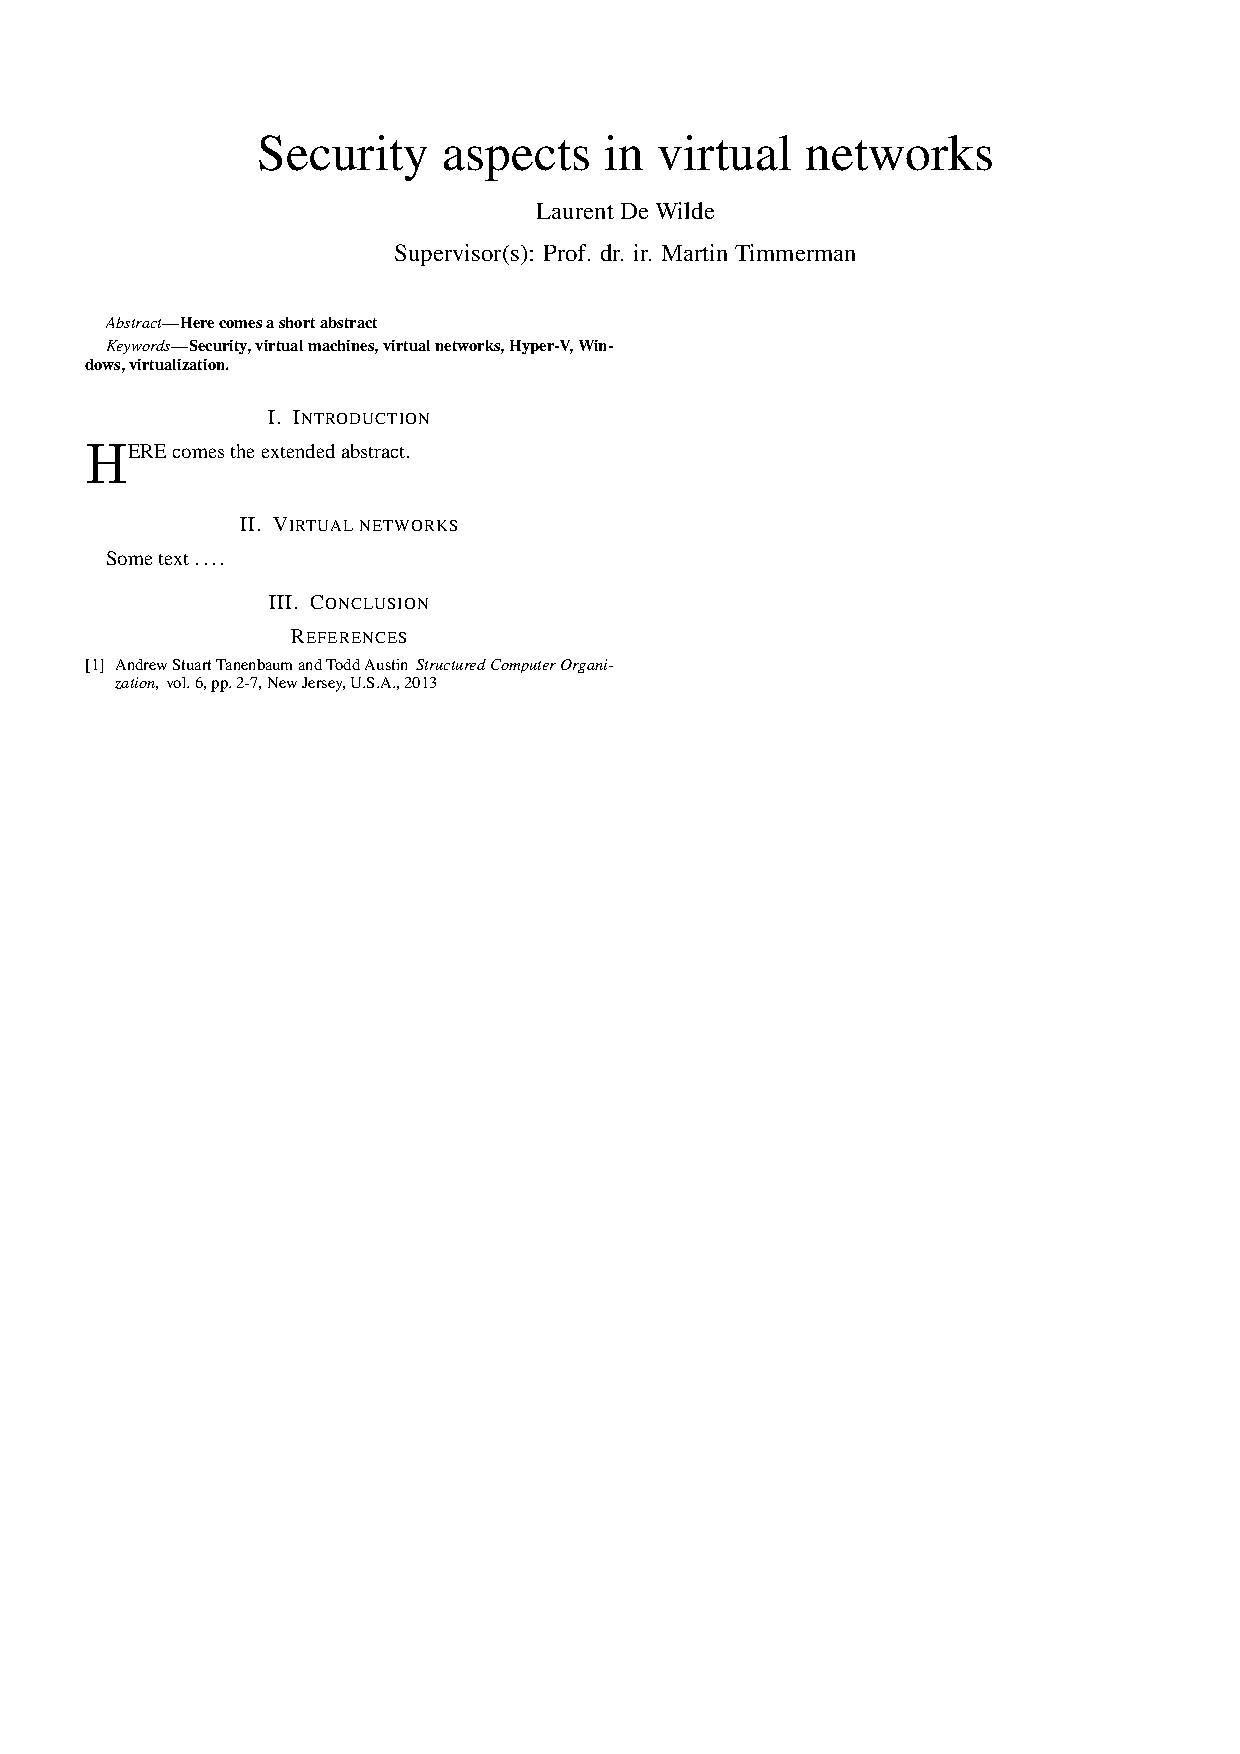
\includepdf[pages=-]{../abstract/abstract.pdf}

\pagestyle{fancy}
\renewcommand{\baselinestretch}{1.08} 	% De interlinie afstand wat verkleinen.
\small\normalsize                       % Nodig om de baselinestretch goed te krijgen.
\addcontentsline{toc}{chapter}{Contents}
\tableofcontents
\renewcommand{\baselinestretch}{1.2} 	% De interlinie afstand wat vergroten.
\small\normalsize
\listoffigures
\listoftables                       % Nodig om de baselinestretch goed te krijgen.
\chapter{List of Abbreviations}
\begin{flushleft}
\renewcommand{\baselinestretch}{1.5}
\small\normalsize
\begin{longtable}{ll}
	DMA & \textbf{D}irect \textbf{M}emory \textbf{A}ccess \\
	ESXi & \textbf{E}lastic \textbf{S}ky \textbf{X} \textbf{i}ntegrated \\
	OS & \textbf{O}perating \textbf{S}ystem \\
	OSI & \textbf{O}pen \textbf{S}ystems \textbf{I}nterconnection\\
	NIC & \textbf{N}etwork \textbf{I}nterface \textbf{C}ard \\
	VM & \textbf{V}irtual \textbf{M}achine \\
	VMBR	& \textbf{V}irtual \textbf{M}achine \textbf{B}ased \textbf{R}ootkit \\
	VMM & \textbf{V}irtual \textbf{M}achine \textbf{M}onitor \\
	VMX & \textbf{V}irtual \textbf{M}achine e\textbf{X}tensions \\
\end{longtable}
\end{flushleft}

\mainmatter
\chapter{Introduction}
\label{chap:introduction}
\emph{In the introductory chapter, some basic aspects of virtualization will pass the revue.}
\section{Virtualization}

\subsection{Abstractions}

Computer systems are built as hierarchies with interfaces that separate levels of abstraction. Those levels of abstraction hide lower-level implementation details, which allows for independant development of each seperate layer and thus simplifying the development and maintanance process \citep{ArchVM}.

To clearify this layered build of computer systems, two examples are provided: one applies to application design, whereas the second example applies to disk storage.
\paragraph{First example} Imaging a higher-level programming language, called \textbf{Language1}. This language consists of classes, methods, variables, etc\ldots . This Language5 is very convenient and understandable for people. However, since computer systems only understand machine language, let us call this \textbf{Language1}, one cannot simply feed this language to the low-level digital circuits and hoping for the program to execute.

In fact, the gap between what is conventient for people and what is convenient for computers tend to be very large. So the need to translate the higher-level code (Language5) to low-level bytecode (Language1) is needed. This is where abstractation layers come in.

Imaging a virtual machine \textbf{Machine1} that accepts Language5. The programs written in Language5 can then be translated of interpreted by a program written in Language1, which can be directly executed on the computer hardware \citep{Tanenbaum}.

However, for practical reasons, those two languages Language5 and Language1 cannot be too different. This means that intermediate Languages and thus virtual machines must exist to interpret of translate Language5 into a more lower-level language \textbf{Language4}. This process of continually and gradually translating higher-level languages into lower-level languages can further be executed until the final, lowest-level language (Language0) is reached  \citep{Tanenbaum}. \\ \\
Each virtual machine is a layer. So in the example given, 5 layers exist to translate a higher-level language into a lower-level one. The bottom-most language is the simplest one that computers understand (i.e.: bytecode) whereas the top-most language is the most sophisticated one.

\paragraph{Second example}

In the case of hard disk abstraction, the operating systems hides (i.e.: abstracts) the addressing details, that is, sectors and tracks, for the application software. This means that, from the application point-of-view, the disk appears as a set of files.

Programmers create, read, modify and delete files without knowing those low-level tracks and sectors. The figure below clearyfies the process.

\begin{figure}[h]
    \centering
    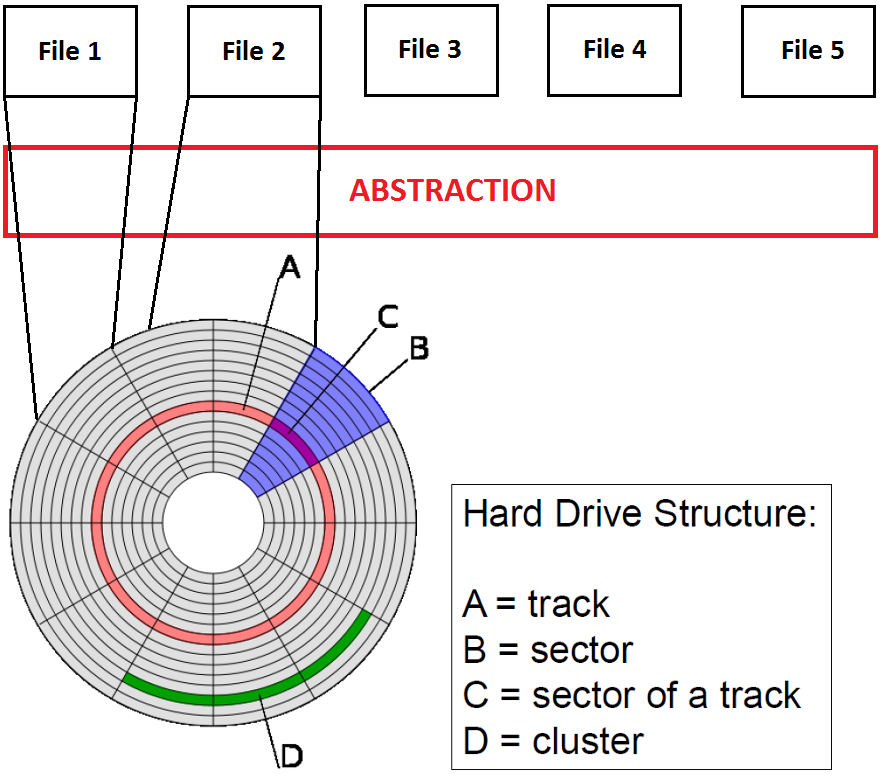
\includegraphics[width=0.65\textwidth]{HD_struct.png}
    \caption[Abstraction applied to disk storage]{Abstraction applied to disk storage. The abstraction layer is in fact the operating system.}
\end{figure}

\clearpage

In fact, not only computer systems are built as hierarchies: also networking systems use several abstractation layers to communicate with each other. What follows is a brief explanation of the OSI model, that describes how network applications may communicate with each other \citep{OSI}.

The OSI model consists of 7 layers as illustrated in the figure below:
\begin{figure}[h]
    \centering
    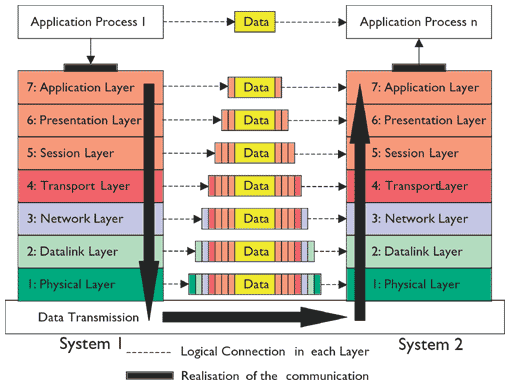
\includegraphics[width=0.65\textwidth]{OSI.png}
    \caption[The OSI model]{The OSI model is another example of abstraction. This time not in computer systems, but in networking.}
\end{figure}
Top-level applications do not communicate directly with each other. Instead, data is passed from one layer to another, starting at the application layer and proceeding to the bottom layer. There, the data is sent over the communication channel to the other host where the whole process takes place in reverse order \citep{OSI2}. 

The seven layers can be seen as abstraction layers. Each layer hides details of the level directly beneith it.

\subsection{Abstraction and virtual machines}

Virtualization exists in many forms. Not only there exist storage (disk) virtualization, but also network virtualization, virtualized applications and hypervisors. In the first case, virtualization does not necessarily aim to hide details \citep{ArchVM}. 

Consider the figure below. Virtualization transforms a physical disk into two smaller disks. Each of those disks appears to have its own tracks, sectors and clusters. Furthermore, the virtualization software uses the file abstraction described in the previous section to map a virtual disk onto the real physical disk.

Data that is to be written onto the virtual disk, is converted to a file write. Since the file resides on the real physical disk, data is actually written to the physical disk.

This is an example of abstraction and virtualization applied to disk storage.
\begin{figure}[h]
    \centering
    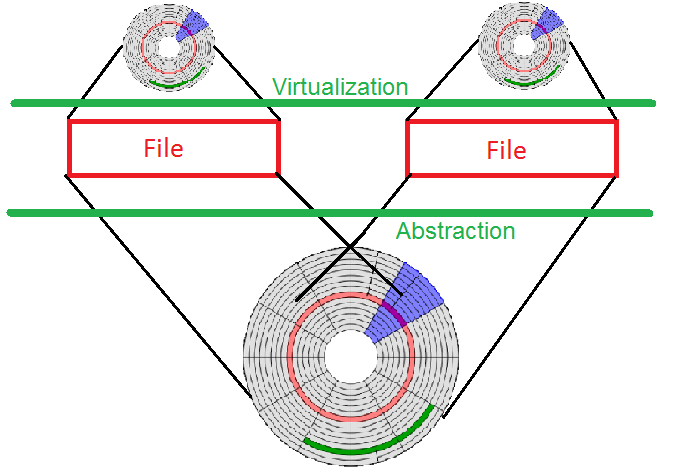
\includegraphics[width=0.65\textwidth]{HD.png}
    \caption[Virtualization of hard disks]{Virtualization applied to disk storage}
\end{figure}
Obviously, the whole concept of (disk) virtualization can also be applied to physical machines. This is where hypervisors make their entry.

A hypervisor will abstract the physical resources, that is, CPU, memory, disk and network, from systems running on top of it \citep{VMIntro1}. This means that those physical resources are shared between the virtual machines and thus allows that multiple virtual machines can run on a single physical machine.

Chapter \ref{chap:virtualnetworks} provides more details about virtualization and hypervisors in particular.

\section{Why use virtualization}

\subsection{Benefits of using machine virtualization}

\begin{itemize}
\item \textbf{Server consolidation} The most prominent advantage of using machine virtualization (where a hypervisor is used to abstract the physical machine resources) is server consolidation. In the case of a typical non-virtualized application server for example, about 5\% to 10\% of the server's hardware is utilized. However, when a server hosts multiple virtual machines, utilization can reach values of 50\% to 80\% \citep{Benefit1}.

The whole point of machine virtualization is that the hardware of the physical machine is used more efficiently. It permits to get more out of the existing, physical hardware, because multiple virtual machines that act as real servers can run on top of one physical machine. This has an important consequence: fewer physical servers can be used to achieve the same goals. This means lower operating costs, e.g.: less power and air conditioning are needed \citep{Benefit2}.
\item \textbf{Easy cloning} In contrast to a physical server, which consists of a mixture of application files, OS files, driver files and user files, a VM exists as a single file \citep{Benefit1}. This file can be duplicated, which leads to easy creation of exactly the same machine (server). Obviously, these images can be modified for each application \citep{Benefit3}.
\item \textbf{High availability} When running multiple virtual machines, the load can be distributed amongst them. When a VM fails, another VM can just be started with ensures minimal downtime or data loss \citep{Benefit3}.
\item \textbf{Scalability} Scalability can greatly be improved using virtual machines. Additional resources can quickly be allocated from the host to the guest \citep{Microsoft}: when a certain task requires more RAM, adding RAM to the virtual machine consist of editing a parameter on the hypervisor, whereas in the case of a physical machine, it can take minutes to add more RAM \citep{Benefit3}.
\end{itemize}

\subsection{Challenges and disadvantages of using machine virtualization}

\begin{itemize}
\item \textbf{Longer recovery in case of physical hardware failure} and therefore longer downtime. When the physical machine breaks down because of a catastrophic hardware failure, all the virtual machines need to wait until the physical host is brung up online, after which the VM's can start booting. This means increased downtime \citep{Benefit3}.
\end{itemize}


\section{Security issues regarding virtualization}
\label{sec:securityRegardingVirtualization}
Consider the VMware ESXi Hypervisor. All virtual machines are isolated from each other \citep{Benefit4}. The advantages of this practise are for example the fact that if one VM fails, the remaining VM's remain accessible or the fact that if one VM gets infected with, let's say, a Trojan Horse, this will not affect the other VM's \citep{CompTia}.

However, this is not entirely true: cases have been reported in where virusses are able to break out VM's \citep{Crossover}. Additionaly, since VM are networked - either internally using a virtual switch or bridged with the physical network (or both), a new thread arises. Malware with a network component (e.g.: worms), travels where their routing tells - or allows - them to go \citep{Stackex}. Therefore , it is perfectly possible that an infected VM might infect other VM's while the network administrator believed this could never happen.

The whole point is that one may not assume that VM's are really isolated from each other and that an infected VM cannot infect another one - even if they are not networked. Chapter 3 will cover security in more detail.\\

In this thesis, virtual networks will be tested against known and unknown security problems concerning virtual networks. Furthermore, securtity aspects will be highlighted in virtual networks. \\ \\
\emph{This chapter briefly described some basic concepts of virtualization, especially machine virtualization. Advantages and disadvantages of virtualization have been discussed as well as a brief mention about security issues related to virtualization.\\
In the next chapter, )}
\chapter{Virtualization}
\label{chap:virtualnetworks}
\emph{In this chapter, (the) three types of virtualization will be explained in detail: machine virtualization, network virtualization and storage virtualization.}

Before digging deeper into security aspects in virtual networks, some types of virtualization must first be defined.
\section{Machine virtualization - Hypervisors}
In order to be able to run virtual machines, a hypervisor is needed. Chapter \ref{chap:introduction} already described the function of a hypervisor, also called a virtual machine manager \citep{Techtarget}: a hypervisor abstracts the physical resources - CPU, memory, disks, network adapters, \ldots - from systems running on top of it. So it allows for a physical machine (that we will call a host) to share their hardware resources amongst virtual machines (that we will call guests) running as guests on top of the host (the physical hardware). Note that a hypervisor is nothing more than a piece of software \citep{Datacenter} that ensures that VM's do not interrupt each other \citep{Techtarget}.

Each VM appears to have it's own processor, memory and disk. However, the hypervisor is actually controlling the VM's resources and allocating the resources to their needs \citep{Techtarget}. 

There exist two types of hypervisors:  \textbf{Type 1} and \textbf{Type 2} hypervisors \citep{Techtarget2}. Type 1 hypervisors are the so-called \textbf{Bare-metal hypervisors} whereas type 2 hypervisors are known as \textbf{hosted hypervisors}. Both will be discussed in the upcoming sections.

From know on, the physical machine will be called the \textbf{host} and the virtual machine that runs on top of the host (through the hypervisor), will be called the \textbf{guest}.

\subsection{Bare-metal hypervisors}
\label{sec:baremetal}
The name `bare-metal' (``without an operating system'') comes from the fact that this type of hypervisor is deployed as a bare-metal installation. This implies that it is not required to first install a server operating system: the hypervisor is the first thing to be installed on the host \citep{Techtarget2}. To be precise: the hypervisor is installed as the operating system of the host \citep{Datacenter}.

A bare-metal hypervisor runs directly on the host's hardware and therefore allow for direct access to the hardware recourses, which results in greater performance compared to hosted hypervisors \citep{Techtarget2} as illustrated in the picture below. One point of remark: the VM's running on top of the hypervisor do not have direct access to the hardware recourses. Instead, they have a virtual view of for example the processor and run in a private memory address region that is unique for each guest \citep{HyperVArch}. Only the hypervisor has direct access to the hardware.

\begin{figure}[h]
    \centering
    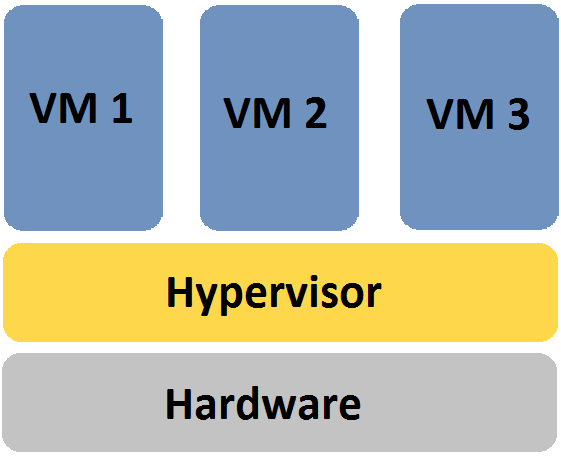
\includegraphics[width=0.55\textwidth]{BareMetal.png}
    \caption[Bare-metal hypervisor]{A schematic architecture of a typical bare-metal hyervisor. As one can see, the hypervisor runs directly on the host's hardware and therefore has direct access to the hardware.}
\end{figure}

\subsubsection{Hyper-V}

Hyper-V is a bare-metal hypervisor developed by Microsoft \citep{HyperV}. Hyper-V is the replacor of Microsoft Virtual PC in newer versions of Windows\citep{HyperVSuccessor} and was first included in Windows Server 2008, where system administrators could enable the Hyper-V role \citep{HyperV2}. Hyper-V only supports x64 versions of Windows Server 2008 and Windows Server 2012 \citep{HyperVArch}.

The Hyper-V role provides the software infrastructure and management tools to create and manage a virtualized computer environment. As previously explained in section \ref{sec:securityRegardingVirtualization}, each VM runs in a isolated computing environment \citep{HyperVOverview}. In Hyper-V, this isolation is achieved by means of partitions \citep{HyperVArch}.

\paragraph{Architecture of Hyper-V}

In order for Hyper-V to work, a root partition (also known as parent partition) must be present on top of the hypervisor running a 64 bit version of Windows Server 2008 or Windows Server 2012. \citep{HyperVArch}. It also runs the virtualization stack, contains the device drivers and therefore has direct access to the hardware resources as well \citep{HyperVArch2}.

In essential, this root partition is nothing more than a virtual machine running Windows Server 2008 or Windows Server 2012 used to control the other guest VM's. The machine that installed the Hyper-V role, becomes the root partition.
The root partition can be compared to the Dom0 VM of the Xen Project hypervisor explained in section \ref{subsub:Xen}. \\ \\
The picture below visualizes the Hyper-V's architecture.
\begin{figure}[h]
    \centering
    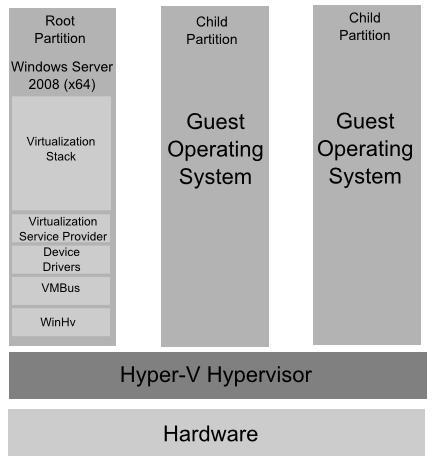
\includegraphics[width=0.55\textwidth]{HyperVArch.jpg}
    \caption[Hyper-V Architecture]{The architecture of the Hyper-V hypervisor. The root partion contains the Virtualization Stack which, in his turn, contains a collection of tools that provide the Hyper-V functionality, for example the virtual devices and the device drivers.}
\end{figure}

%\paragraph{Scheduling in Hyper-V}

\clearpage

\subsubsection{Xen}
\label{subsub:Xen}
The Xen Project hypervisor is the only open source bare-metal hypervisor available at the time of writing. It consists of four main components being the Xen Project hypervisor, the guest VM's, the Control Domain and the Toolstack \citep{Xen1}. \\
\paragraph{Architecture of the Xen Project hypervisor}
The Xen hypervisor runs directly on the hardware and contains the scheduler. It is responsible for handling interrupts, CPU time and memory usage. The hypervisor is the first program to run after exiting the bootloader \citep{Xen1}.\\ \\
The Control Domain (Dom0) is a special type of virtual machine. Compared to the other guest VM's, this Dom0 has special privileges. E.g.: it is able to access the hardware directly and interacts with the other VM's. Therefore, the Dom0 contains the drivers for the hardware and a toolstack \citep{Xen1}.

One could compare this Dom0 with the root partition of Hyper-V.

The Dom0 is the first VM to be started by the hypervisor.\\ \\
The Toolstack (xl is the prefered toolstack at the time of writing \citep{Xen2}) allows users to manage their VM's \citep{Xen1}.\\ \\
The guest VM's run on top of the Xen hypervisor and run their own operating system and application software. These are the actual VM's. \\
The picture below visualizes the Xen Project hypervisor's architecture \citep{Xen2}.
\begin{figure}[h]
    \centering
    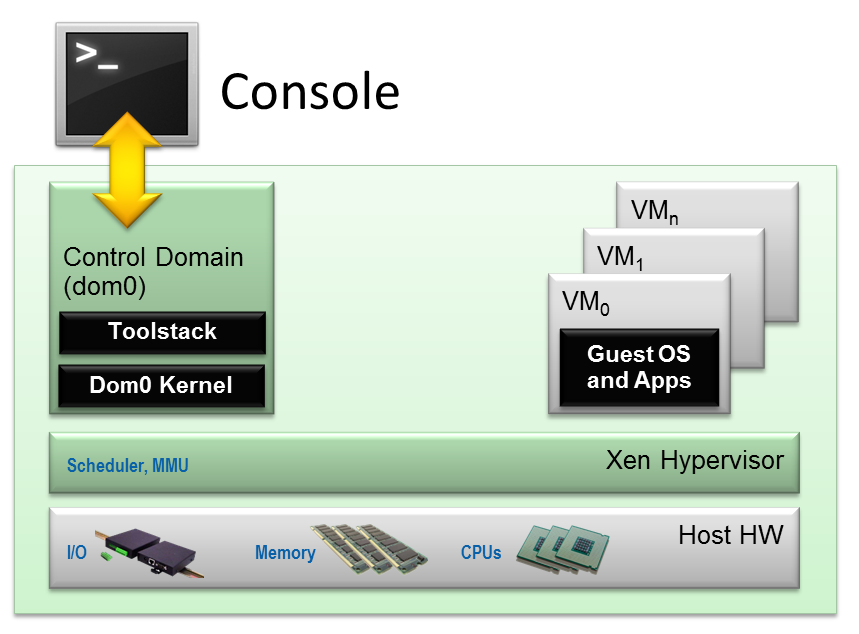
\includegraphics[width=0.45\textwidth]{Xen_Arch_Diagram.png}
    \caption[Xen architecture]{The architecture of the Xen Project hypervisor. It consists of four main components: the hypervisor itself, the guest VM's, the Control Domain and the Toolstack for managing the VM's.}
\end{figure}

\clearpage

\subsubsection{VMware ESXi}

VMware ESXi the bare-metal hypervisor developed by VMware. It is the successor of the ESX hypervisor \citep{VMware1}.

\paragraph{Architecture of the ESXi hypervisor}

The VMware ESXi hypervisor consists of the VMkernel, which is the underlying operating system and processes that run on top of the VMkernel.

The VMkernel contains the drivers, the management agents and applications and hardware monitoring components. The processes run on top of it are the Direct Console User Interface (DCUI), the virtual machine monitor (VMM) together with the helper processes VMX. Each VM has its own VMM and VMX process.
On top of the VMkernel run the guest VM's. \\ \\
The DCUI is responsible for low-level configuration and management. It is accessible through the server console and is used for basic, initial configuration.

The VMM is a process that provides an execution environment for the virtual machines, together with some helper processes knows as VMX processes.

Note that - in contrast to Hyper-V and Xen, there does not exist a fully functional console OS that manages the VM's. Instead, only a small POSIX kernel is included. This implies that the footprint of the hypervisor is very small - not more than 32MB.

\begin{figure}[h]
    \centering
    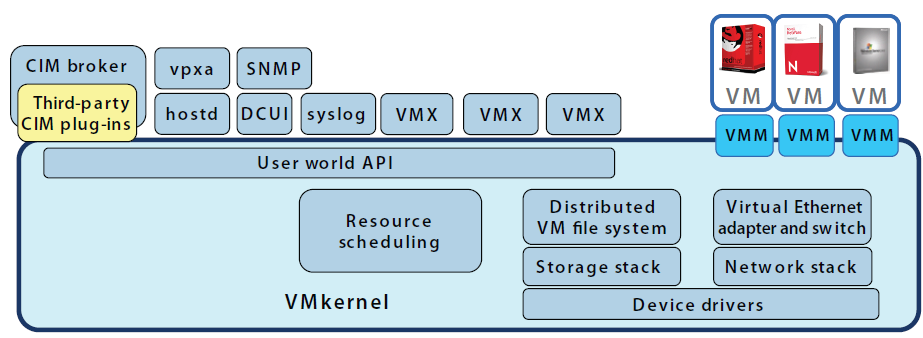
\includegraphics[width=0.65\textwidth]{VMware1.png}
    \caption[VMware architecture]{...}
\end{figure}
 \clearpage
\begin{figure}[h]
    \centering
    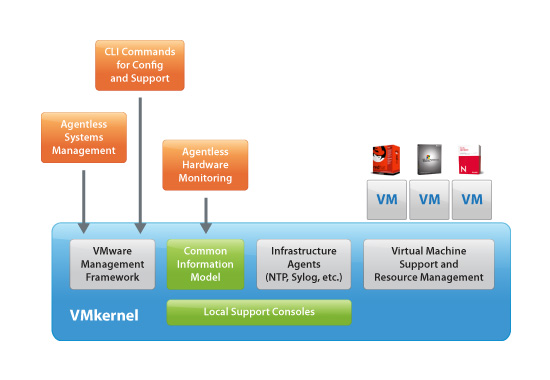
\includegraphics[width=0.55\textwidth]{VMware2.jpg}
    \caption[VMware simplified architecture]{...}
\end{figure}


The architectures of these 3 hypervisors are roughly equal \ldots .
In this thesis, Hyper-V will be used.
\subsection{Hosted hypervisors}

As described in section \ref{sec:baremetal}, bare-metal hypervisors run directly on top of the hardware. However, another type of hypervisor exist that runs on top of an existing operating system: the hosted hypervisors or type-2 hypervisors.

So basically, this means that an operating system is installed inside another operating system in contrast to the bare-metal hypervisor where each OS has direct access (through the hypervisor) to the hardware.

An example of such a hosted hypervisor is VirtualBox \citep{VirtualBox}.

\section{Network virtualization}

After having defined virtual machines and the hypervisors, it is now time to focus how a virtual machine is able to communicate with the outside world and to have a closer look how internal (i.e.: inside the hypervisor) network virtualization works. \\ \\
When one wants to provide a VM with network capabilities, at lease one virtual network interface card (vNIC) has to be assigned to this VM - just as a physical computer requires a physical NIC as well  \citep{Technet1}.

As Hyper-V will be used in this thesis, the focus of internal virtual networking will be stressed on Hyper-V. \\ \\

One must not forget that a virtual network is actually just a software logic that is part of Hyper-V and sents and receives packets in OSI layer 2. \\

There exist three different types of virtual networks in Hyper-V: external virtual networks, internal virtual networks and private virtual networks \citep{HyperVNetworking2}. Each of them will be explained in the following section.

\subsection{External virtual network}

Virtualization is all about abstracting existing hardware as explained in the first chapter. The same concept is used for virtual networking. Consider a host with an arbitrary number of cores and an arbitrary amount of RAM which hosts 50 VM's, but with only one physical NIC.

The requests performed by the virtual NIC's of the VM's can overhelm the physical NIC of the host. To overcome this problem, Microsoft developed an abstraction layer that uses the Virtual Switch concept \citep{HyperVNetworking1}.

This abstraction layer sits in between the the physical NIC and the vNIC's of the different VM's. It therefore abstracts the physical NIC. Microsoft calls this \emph{External Networking} \citep{HyperVNetworking2} and is illustrated in the figure below \citep{HyperVNetworking1}.\\
\begin{figure}[h]
    \centering
    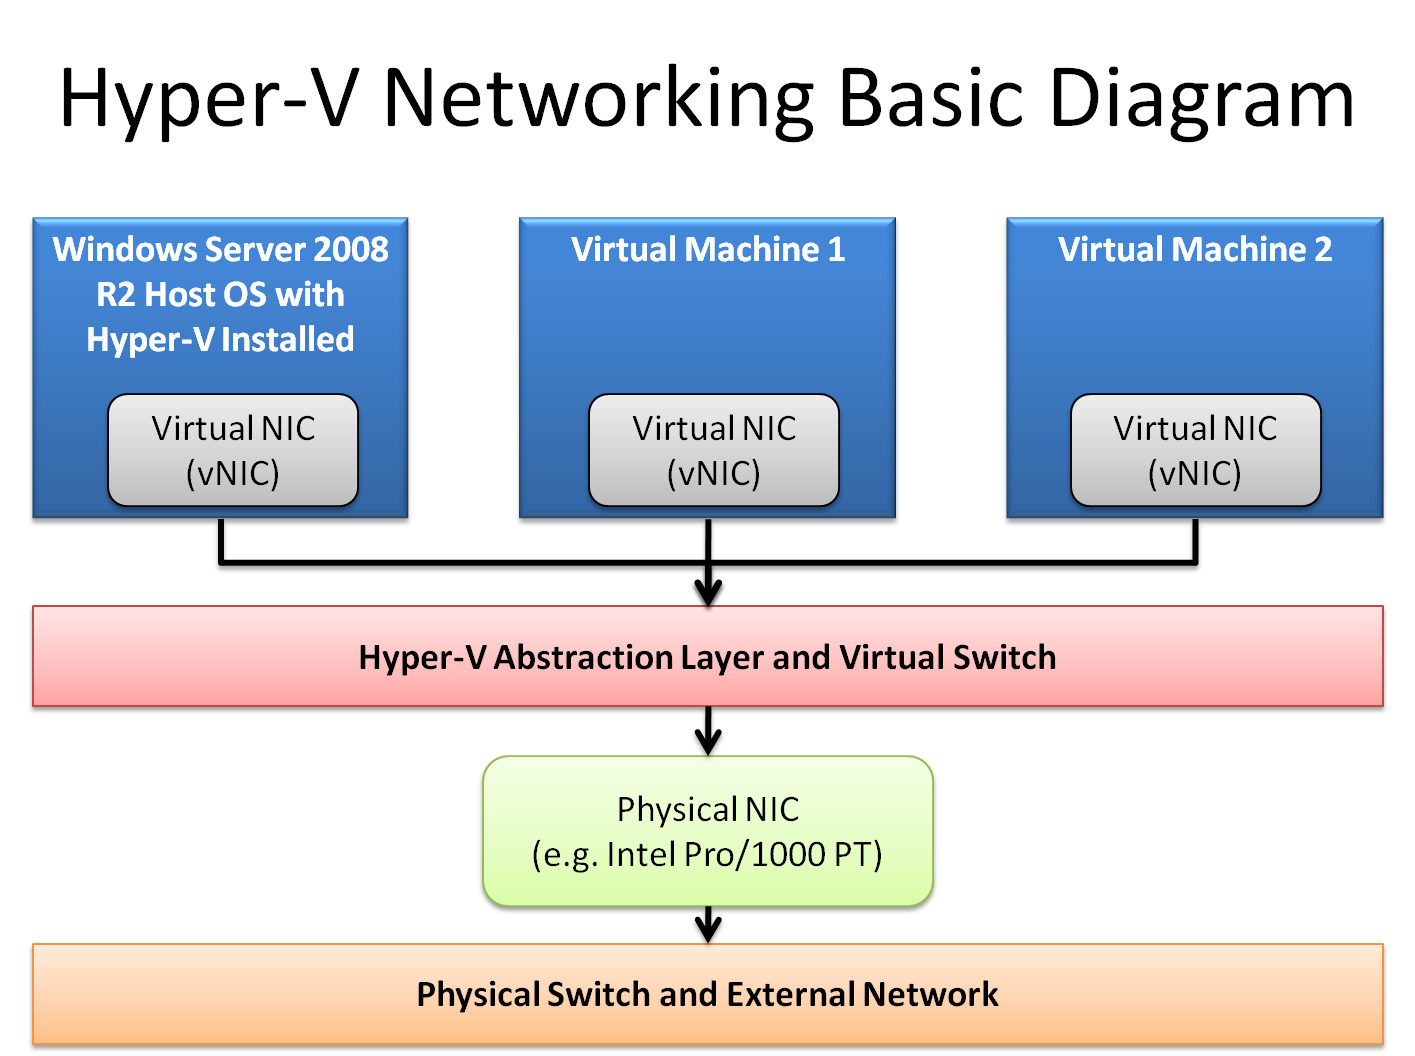
\includegraphics[width=0.65\textwidth]{ExternalNetwork.png}
    \caption[Microsoft Virtual Switch concept]{The concept of virtual networking as an abstraction layer on top of the physical NIC. The purple layer represents the virtual switch. Note that this is only occurs with external networking - internal and private networking do not use virtual switches.}
\end{figure}
When creating an external virtual network in Hyper-V, the following changes take place:
\begin{itemize}
\item The host creates a new virtual NIC that is used to connect to the physical network. So a minimum of two network adapters exist on the host.
\item The Microsoft Virtual Switch Protocol is bound to the physical NIC.
\end{itemize}
Once created, the virtual network will work exactly the same as a phyiscal network, with that difference that the switch is a software-matic; additional ports (NICs) can be added dynamically.
Following figure visualizes the external network concept of Hyper-V.
\begin{figure}[h]
    \centering
    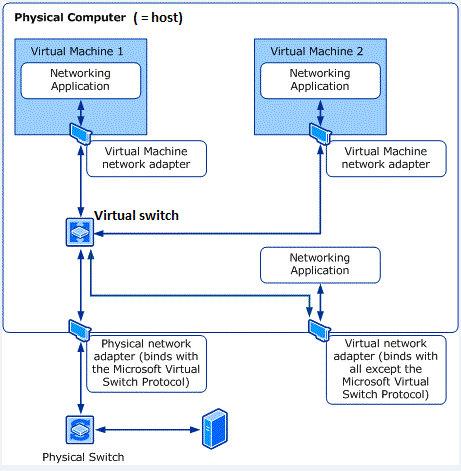
\includegraphics[width=0.65\textwidth]{ExternalNetwork_2.png}
    \caption[External Virtual Network]{A diagram of the different components of external networking. The physical NIC binds with the virtual switch. The networking applications of the host communicate with the external network (the physical switch) through the newly created virtual NIC. Note that each VM is assigned a virtual NIC.}
\end{figure}
The external network type has the following capabilities \citep{HyperVNetworking3}:
\begin{itemize}
\item It allows for communication between a VM and and an external network so that all VM's are visible as seperate hosts on the external network  as if they would be dedicated, physical hosts. One can compare this with Xen bridged networking \citep{XenNetworking}.
\item It allows for communication between VM's on the same host.
\item It allows for communication between the VM's and the host.
\end{itemize}

\subsection{Internal virtual network}

In an internal virtual network, the phyiscal adapter plays no role in the network and is therefore not bounded. Thus access and communication to external networks (including the LAN outside the virtual machine) is impossible \citep{HyperVNetworking1, HyperVNetworking3}. However, communication with the host is possible. \\
Some characteristics of internal networks are \citep{HyperVNetworking2}:
\begin{itemize}
\item It allows for communication between VM's on the same host.
\item It allows for communication between VM's and the host.
\end{itemize}
The figure below visualizes this concept \citep{HyperVNetworking2}:
\begin{figure}[h]
    \centering
    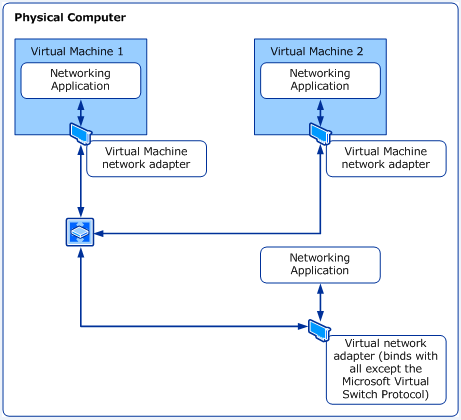
\includegraphics[width=0.65\textwidth]{InternalNetwork.png}
    \caption[Internal Virtual Network]{...}
\end{figure}

\subsection{Private virtual network}

When a private virtual network is used, VM's are only able to communicate with each other. No communication with the host exist, however. That is the difference with an internal private network. \\
Some characteristics of internal networks are \citep{HyperVNetworking2}:
\begin{itemize}
\item Communication between VM's only.
\end{itemize}
he figure below visualizes this concept \citep{HyperVNetworking2}:
\begin{figure}[h]
    \centering
    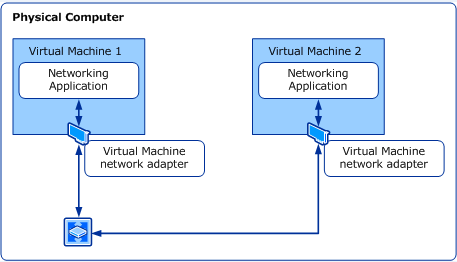
\includegraphics[width=0.65\textwidth]{PrivateNetwork.png}
    \caption[Private Virtual Network]{...}
\end{figure}

\subsection{External network virtualization}

VLAN's, \ldots . Moet aan de prof vragen of dit ook moet.

\clearpage

\section{Storage virtualization}

\subsection{Host-based storage virtualization}

Host-based storage virtualization adds, as any virtualization technique (see chapter \ref{chap:introduction}), a layer of abstraction between the host OS and the physical disks. Each mayor OS provides a piece of software called a logical volume manager to provide such a layer of abstraction \citep{VHD3}. \\
Whereas in traditional disk management, the OS looks for physical disks and partitions that reside on those physical disks, with a logical volume manager disks can be abstracted. This way, a logical disk can span multiple physical disk and appear in the OS as one disk.

A logical volume manager adds more flexibility in a way that logical volumes can be resized and moved around. This is not a straightforward job when physical disks and partitions are used \citep{VHD2}. \\
Microsoft's implementation of logical volume management is called Logical Disk Manager. In the next section, virtual hard disks in Hyper-V will be discussed. \\
The next figure illustrates the concept of Logical Volume Management.
\begin{figure}[h]
    \centering
    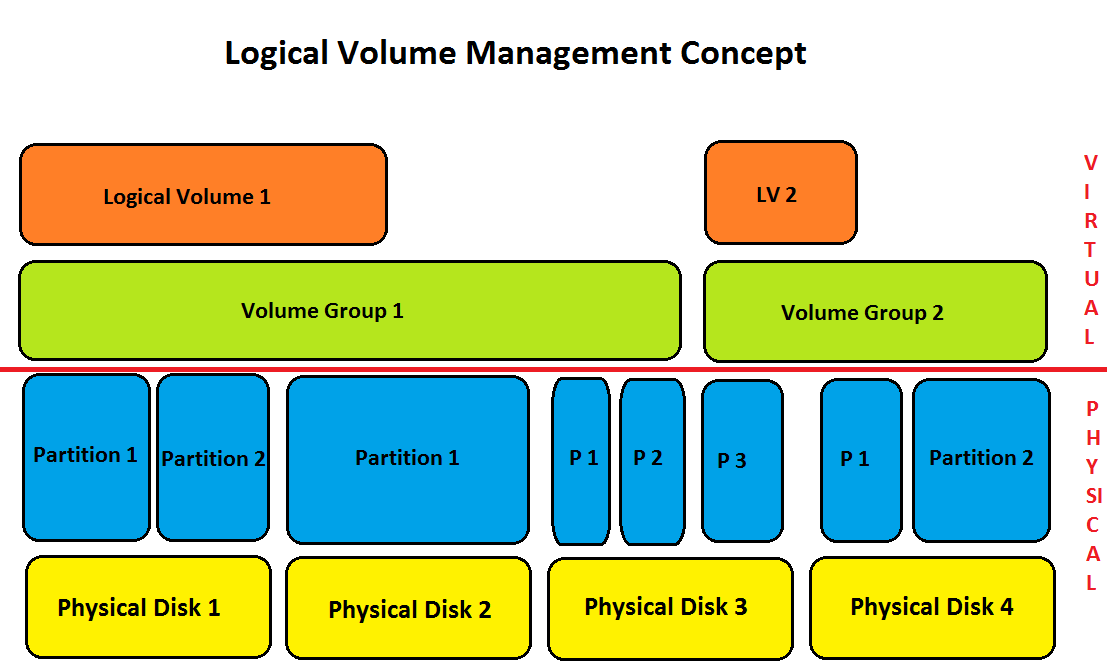
\includegraphics[width=0.85\textwidth]{LVM.png}
    \caption[Logical Volume Management]{LVM adds a layer of abstraction between the OS and the phyical disks / partitions. In the figure, a volume group spans 5 physical partitions and disks. On top of the volume group lies a logical volume (partition). As one can see, there is space left on the volume group and thus expanding the logical volume (partition) is possible. With a phyiscal partition, this would not be possible without losing data.}
\end{figure}
\subsection{Virtual hard disks in Hyper-V}

A virtual hard disk (with extension .vhd) enables one to create a virtual disk which resides on the physical disk as a single file \citep{VHD1}.
A VHD has the same capabilities as a physical disk and thus are used the same way. They are able to host file systems and support standard disk operations \citep{VHD1}.
\chapter{Security aspects}
\label{chap:security}
\emph{In this chapter, some security issues concerning virtual machines and virtualization in general are covered, which will be the basis for further research in this MA thesis.}

\section{Known non-network related security issues}

\subsection{Virusses and malware problems}

The main question we ask ourself here is the fact that if it is possible that virusses and rootkits can be transmitted from a guest VM to the host without the VM having networking capabilities? \\

As seen in the first section, virtual machines are all isolated from each other. Thus, it might seem odd that breakouks are likely to occur. However, with recent advances in technology as x86 Virtualization and I/O MMU Virtualization it turns out this is in fact possible. \\

\paragraph{I/O MMU Virtualization and DMA} With I/O MMU Virtualization, for example Intel VT-d \citep{VTD} or AMD-Vi \citep{AMDVI} it becomes possible to directly assign an I/O device such as a graphical adapter to a VM \citep{HardwareVirt4}. But it also enables Direct Memory Access (DMA). One does not have to be a security expert to see that an infected VM with Direct Memory Access can infect the memory of the host.

\clearpage

\paragraph{x86 Virtualization and rootkits} Noticable rootkits \footnote{\textbf{Rootkit:} a mostly malicious program that is designed to hide itself for detection and thus for the fact that an OS has been compromised. It is used to gain \emph{root} access (hence the name) to the compromised OS to perform, for example, eaves-dropping \citep{VMBR, Rootkit}.} are the \textbf{Blue Pill} rootkit developed by Joanna Rutkowska and the \textbf{SubVirt rootkit}, developed by Microsoft. These rootkits are two examples of VM-based rootkits (VMBR), which install an additional VMM between the host hardware and an existing operating system \citep{BluePill,LibVirt}, after which this new VMM can be used to host malicious software as illustrated in figure \ref{fig:LibVirt}.  Additionally and in contrast to usual rootkits, hypervisor-level rootkits remain undetectable, because they cannot be accessed by software \citep{BluePill,VMBR}.

One possible solution to minimize (the bluepill attack becomes impracticable) this problem from happening is to disable x86 virtualization \footnote{\textbf{x86 virtualization:} also known as hardware-assisted virtualization \citep{HardwareVirt1}, improves the performance when full virtualization is used. It adds hardware support to run VM's more efficiently. Normally, the machine code of the guest OS is translated to machine code of the host OS, by means of binary translation. With x86 virtualization - or hardware-assisted virtualization, the need for such binary translation disappears. Hardware-assisted virtualization must be supported by the CPU \citep{HardwareVirt3}. Therefore, for example Intel and AMD developed respectively Intel-VT and AMD-V for that purpose \citep{HardwareVirt2}}, despite the loss in performance. Also bear in mind that an anti-virus scanner on the host does not protect a guest VM against virusses \citep{Virus}. 
\begin{figure}[h]
	\label{fig:LibVirt}
    \centering
    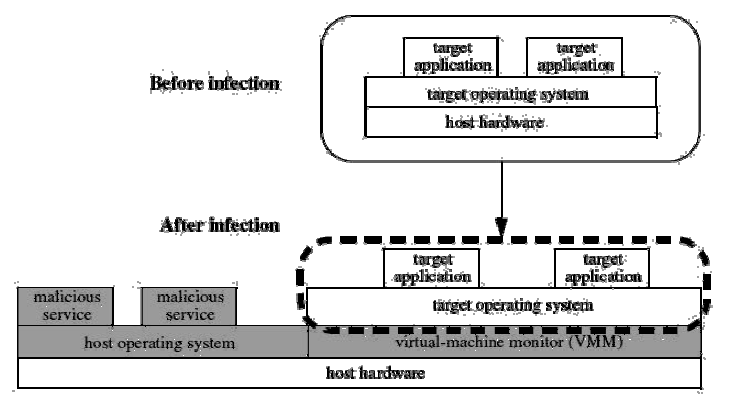
\includegraphics[width=0.7\textwidth]{VMBR.png}
    \caption[VM based rootkit]{A schematic view of a virtual machine based rootkit (VMBR). A VMM, for example Hyper-V, is installed underneath an existing OS. This means that the rootkit is now the hypervisor.}
\end{figure}

\clearpage

\section{Known network related security issues} 

When VM's are directly connected to an external network (e.g.: using Hyper-V's external network mode), then the VM is threated as any other physical machine regarding the transmission of virusses. Just a virusses spread between physical machines using files (e.g.: via mail attachments or software downloads) that are transferred through the network \citep{Virus}, the same can also happen with VM's who are connected to an external network, since when a virtual network is connected to a physical NIC, it is exposed to the same threads and security risks as that physical NIC and thus as a normal physical network\citep{Virus2}.

\section{Possible solutions}

\subsubsection{Use of firewalls}

The built-in Windows Firewall in Hyper-V does not interfere - and thus does not protect guests - with guest traffic in any way. Packets will just pass the Windows Firewall without being analyzed, because of the physical adapter bound to the virtual switch is unbound from anything that Windows Firewall has access to. \\ \\
However, extensions to the Hyper-V Virtual Switch are available that take care of these problems. A network packet filter and an intrusion detection or firewall are two out of four examples of such extensions \citep{Firewall1}.

Obviously, one can always completely isolate virtual networks from each other - and from physical networks - in order to protect the host. This can be done using VLAN's - or IP subnets - : the hypervisor (host) does not have to be on the same VLAN as the guests and thus placing it in a seperate VLAN is perfectly possible \citep{Firewall2}.


\subsubsection{Securing the guests}

As already described in the first section, virtual machines are isolated from each other, in such a way they cannot access each other's physical resources such as RAM.

However, in 2012, a security issue was found in 64 bit virtualization software running on Intel CPU's. With this vulnerability, when a system exception occured, it became possible to escape from the local guest OS into the host OS with elevated privileges, with all the consequences.

Therefore, a guest has to be secured and securing a guest is just like securing a phyiscal machine.

\subsubsection{Antimalware solution}

Attention has to be payed when installing antimalware solutions on the host OS. Either antimalware solution poses a threat to the host: most of the antimalware software dislike XML files, however, these files defines the VM's, so deleting them will cause the VM's to disappear.

This means that one has to be very careful when installing antimalware solutions and in particulary take care of exclusions.

\section{Sniffing on virtual networks}

Another potential security hazard is the possibility to snif a virtual network interface to run a network packet analyzer such as Wireshark to capture all the traffic intented for that host and reconstruct the protocols.

An even bigger security risk is that an intruder could possibly hack a virtual switch to set up a trunk port that is able to see the network traffic on the other ports and redirect this traffic to the virtual network interface the intruder is listening on. \\ \\
Actually, the fact that both Hyper-V and Xen are using virtual \textbf{switches} rather than virtual \textbf{hubs} is a first layer of protection.

Indeed, a switch only forwards the traffic to the intented host - since only one host per segment is present, whereas a hub sends an incoming packet to all ports - since multiple hosts can reside on one network segment. \\ \\
In the upcoming sections, the possibilities of packet sniffing on Hyper-V and Xen virtual networks will be examined as well as measures to prevent packet sniffing, thus enhancing the security.

\subsection{First research question: sniffing a virtual NIC}

Following the above mentioned security risks, the first research question is thus \emph{\textbf{if it is possible to snif a virtual network interface and run a network packet analyzer on it?}} and additionally \emph{\textbf{is it possible to hack a virtual switch to capture all the traffic?}} \\ \\
For the purpose of investigating this research question, a test lab has been created. The reader is invited to take a look at figure \ref{fig:network} for a schematic logical overview of the network used in the investigation. Appendix \ref{app:network} contains a detailed description of the hardware used. \\ \\
Before hacking the virtual switch, we must first determine if it is possible at all to snif a virtual network interface - that is, running a network packet analyzer on it?

\subsubsection{Setting up the environment and testing}

Consider the following environment: one Hyper-V host running three VM's. Two of these VM's are ordinary VM's and one is a so-called \texttt{Monitoring VM}, which runs a packet analyser - or any other sniffing / capturing software. \\
Each VM has one virtual NIC and are connected to the external switch of Hyper-V. This means that each VM has access to the lab network and is thus acting as a normal physical device. The picture below represents the reader with a visual representation of the network.
$\;$ \\ \\
\noindent\begin{minipage}{\textwidth}
    \centering
    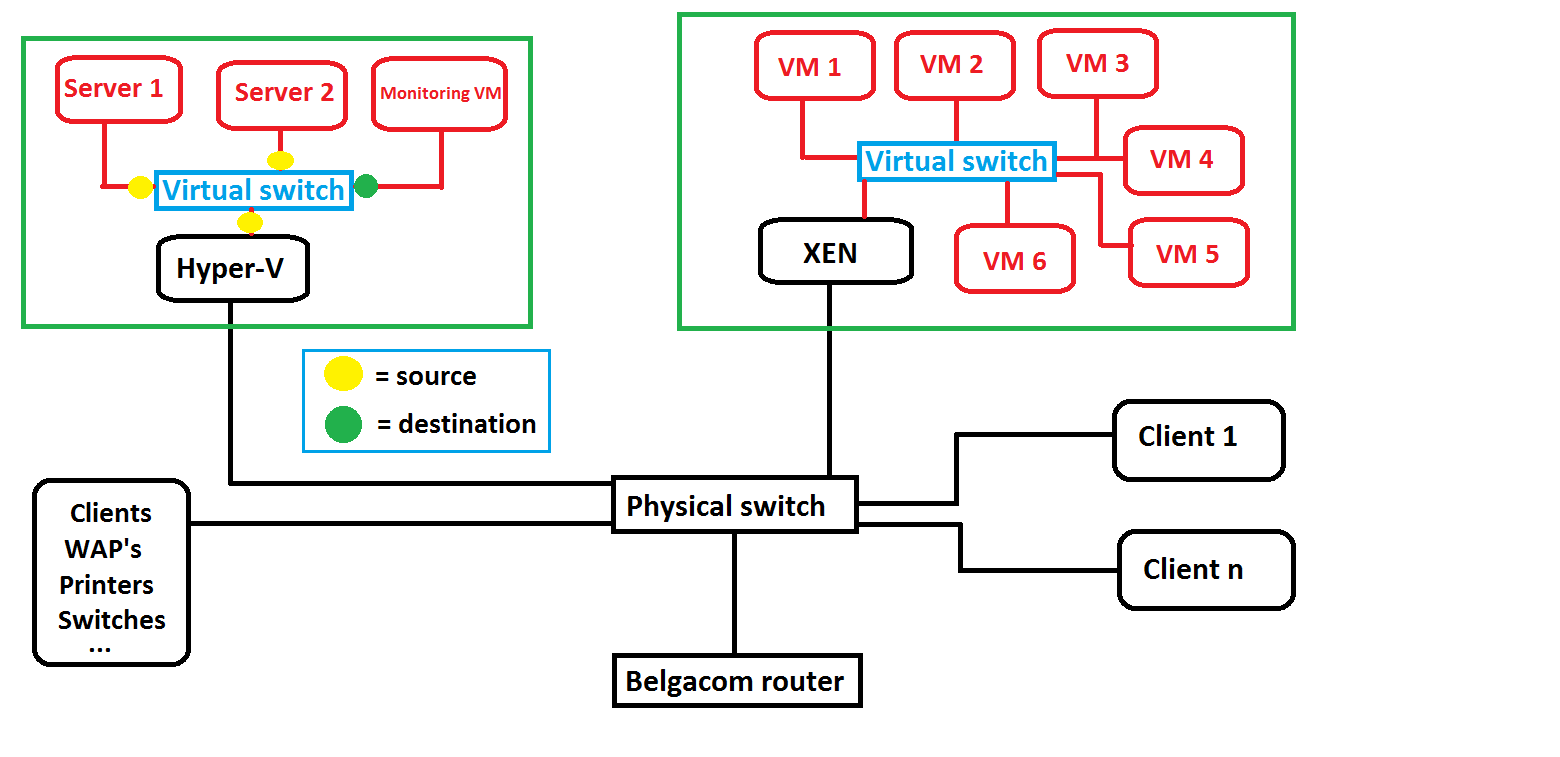
\includegraphics[width=\textwidth]{Network_10.png}
    \captionof{figure}{The network setup used to investigate packet sniffing.}
\label{fig:network}
\end{minipage}
$\;$ \\ \\
After doing some research, it turns out that Hyper-V 2012 has built-in port mirroring. Using this feature, one can set a source interface and a destination interface. All traffic coming from and to the source interface is then copied to the destination interface. (NOG ONDERZOEKEN OF DIT KAN GEWIJZIGD WORDEN BIJ EEN REEDS DRAAIENDE VM) \\ 
Any person with Administrator privileges is able to change the monitoring mode of a VM (that is, a vNIC). This way, when a hacker has gained Administrator access, he could create a new VM with port mirroring configured, or configure port mirroring on an existing VM and install a packet sniffer on it to reconstruct protocols. \\
The figure below illustrates the necessary commands to setup port mirroring on Hyper-V. The first three commands are straightforward, but the last two commands are neccesary to forward traffic that arrives at the Hyper-V external switch interface to the virtual switch. Without these rules, any traffic arriving at the Hyper-V host will `stop' at the host and thus won't be picked up by the \texttt{Monitoring VM}.
$\;$ \\ \\
\noindent\begin{minipage}{\textwidth}
    \centering
    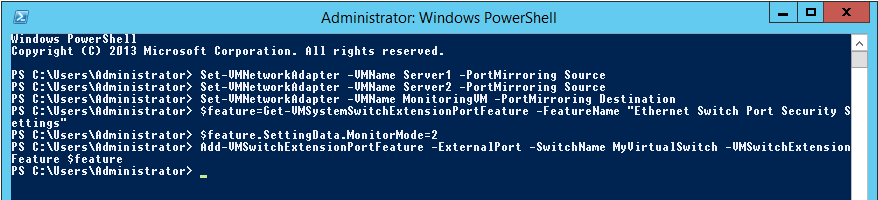
\includegraphics[width=\textwidth]{HyperV_13.png}
    \captionof{figure}{PowerShell commands to configure port monitoring. The vNICs of \texttt{Server 1} and \texttt{Server 2} are set as `source', whereas the vNIC of monitoringVM is set as `destination'.}
\label{fig:network}
\end{minipage}
\paragraph{First stage: inter-VM testing}
After executing the commands, the setup was tested. Wireshark was installed on the \texttt{Monitoring VM} and I pinged from \texttt{Server 1} to \texttt{Server 2} and watched how Wireshark captured all the ICMP Ping requests and replies - not destinated to the \texttt{Monitoring VM}. So, \textbf{yes}, the vNIC on the \texttt{Monitoring VM} captured traffic between VM's (inter - VM) on the same physical host and thus act as a sniffer.
$\;$ \\ \\
\noindent\begin{minipage}{\textwidth}
    \centering
    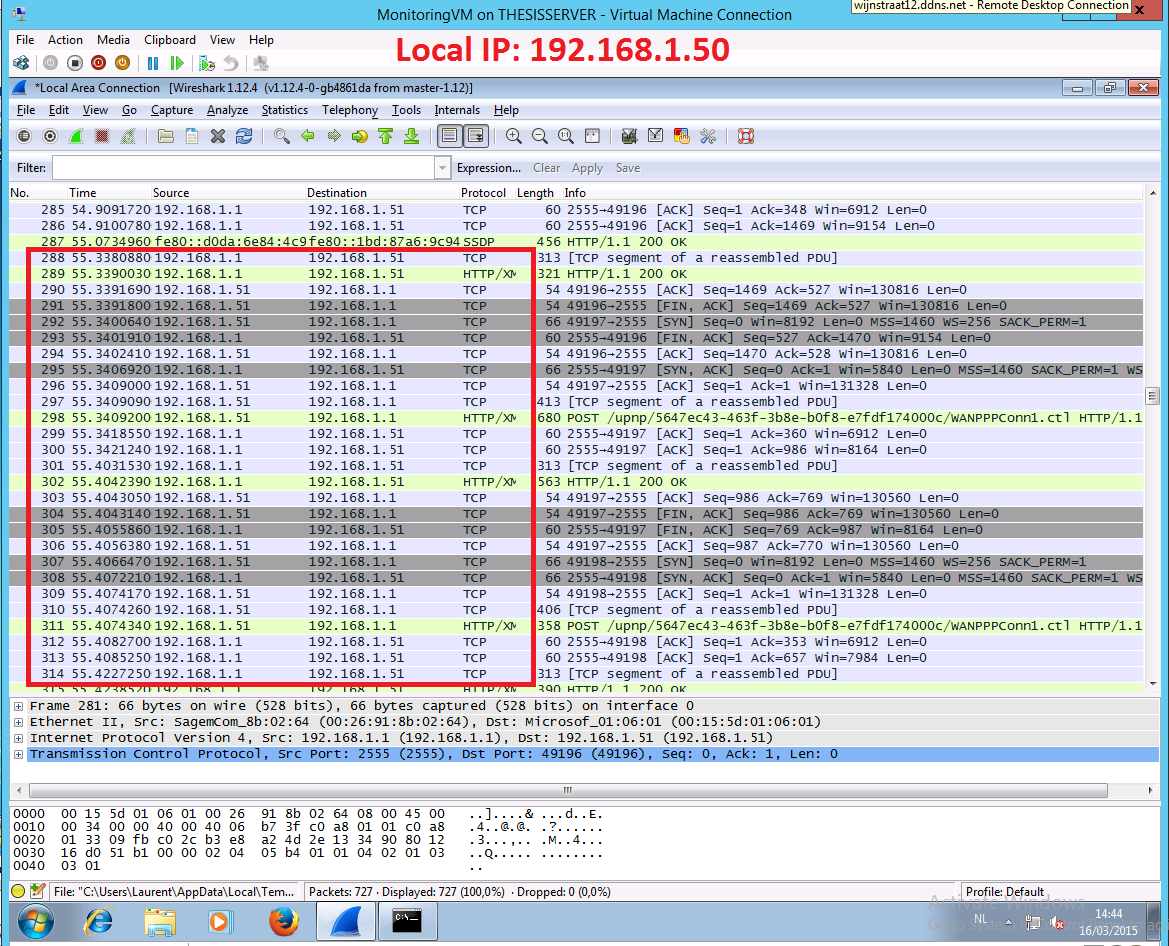
\includegraphics[width=\textwidth]{HyperV_6.png}
    \captionof{figure}{Traffic captured on the Hyper-V virtual network prior to executing the ICMP Ping requests.}
\label{fig:network}
\end{minipage}
$\;$ \\ \\
\noindent\begin{minipage}{\textwidth}
    \centering
    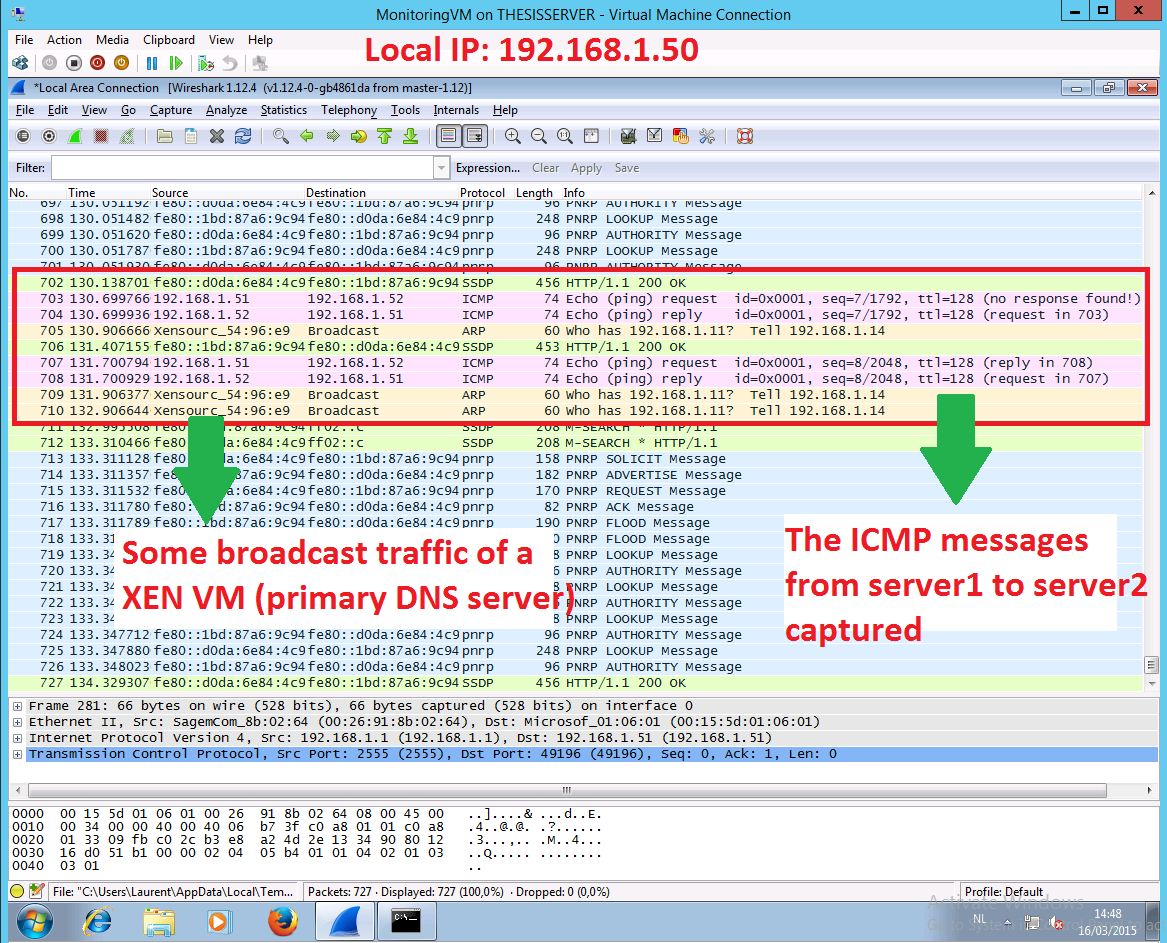
\includegraphics[width=\textwidth]{HyperV_8.png}
    \captionof{figure}{ICMP Ping traffic captured by the monitoring VM. Besides this, some DNS traffic can be observed as well.}
\label{fig:network}
\end{minipage}
$\;$ \\ \\
\paragraph{Second stage: external network testing}
So far, only internal traffic between VM's has been tested for sniffing. I also wanted to test if this \texttt{Monitoring VM} is able to capture traffic originating from the Xen server or any other client on the network.
Therefore, extra ICMP Ping commands have been executed from a random Xen VM to the Hyper-V host as well as to either VM running on this Hyper-V host as illustrated in the following figures.
\noindent\begin{minipage}{\textwidth}
    \centering
    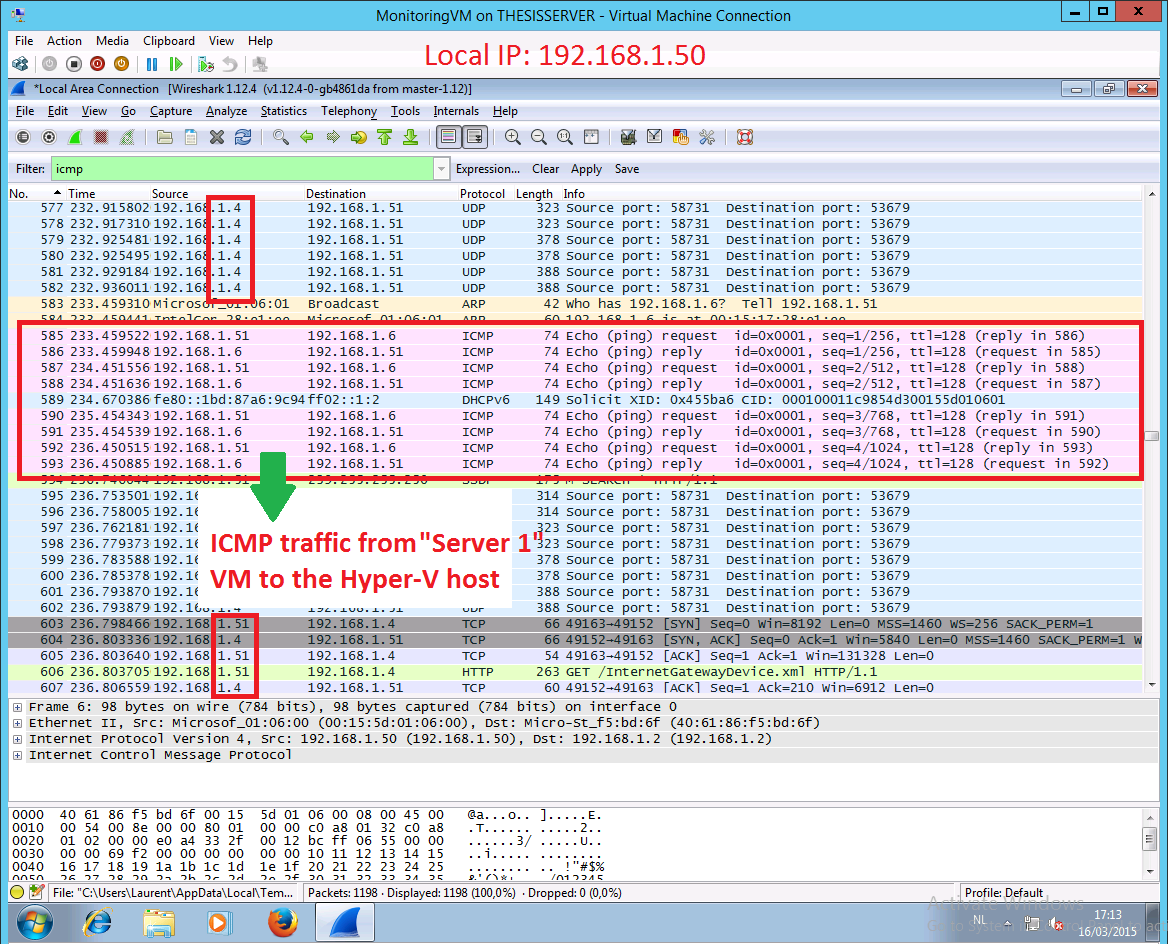
\includegraphics[width=\textwidth]{HyperV_10.png}
    \captionof{figure}{ICMP Ping traffic from \texttt{Server 1} (192.168.1.51) to the Hyper-V host (192.168.1.6). Note that other `external' traffic is captured as well. In this case, traffic from \texttt{Server1} to a wireless access point.}
\label{fig:network}
\end{minipage}
$\;$ \\ \\
\noindent\begin{minipage}{\textwidth}
    \centering
    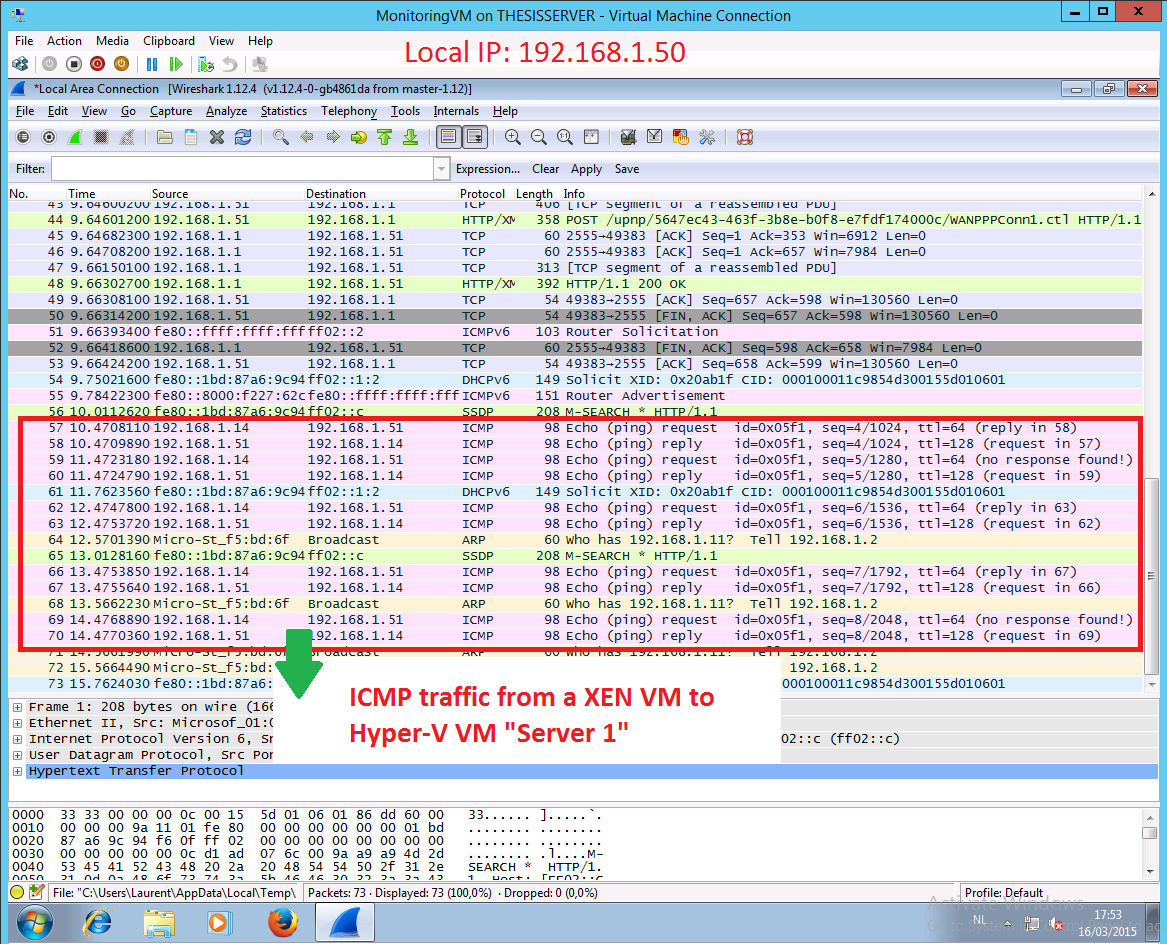
\includegraphics[width=\textwidth]{HyperV_11.png}
    \captionof{figure}{ICMP Ping traffic captured from a Xen VM to a Hyper-V VM, in this case \texttt{Server1}.}
\label{fig:network}
\end{minipage}
$\;$ \\ \\
\noindent\begin{minipage}{\textwidth}
    \centering
    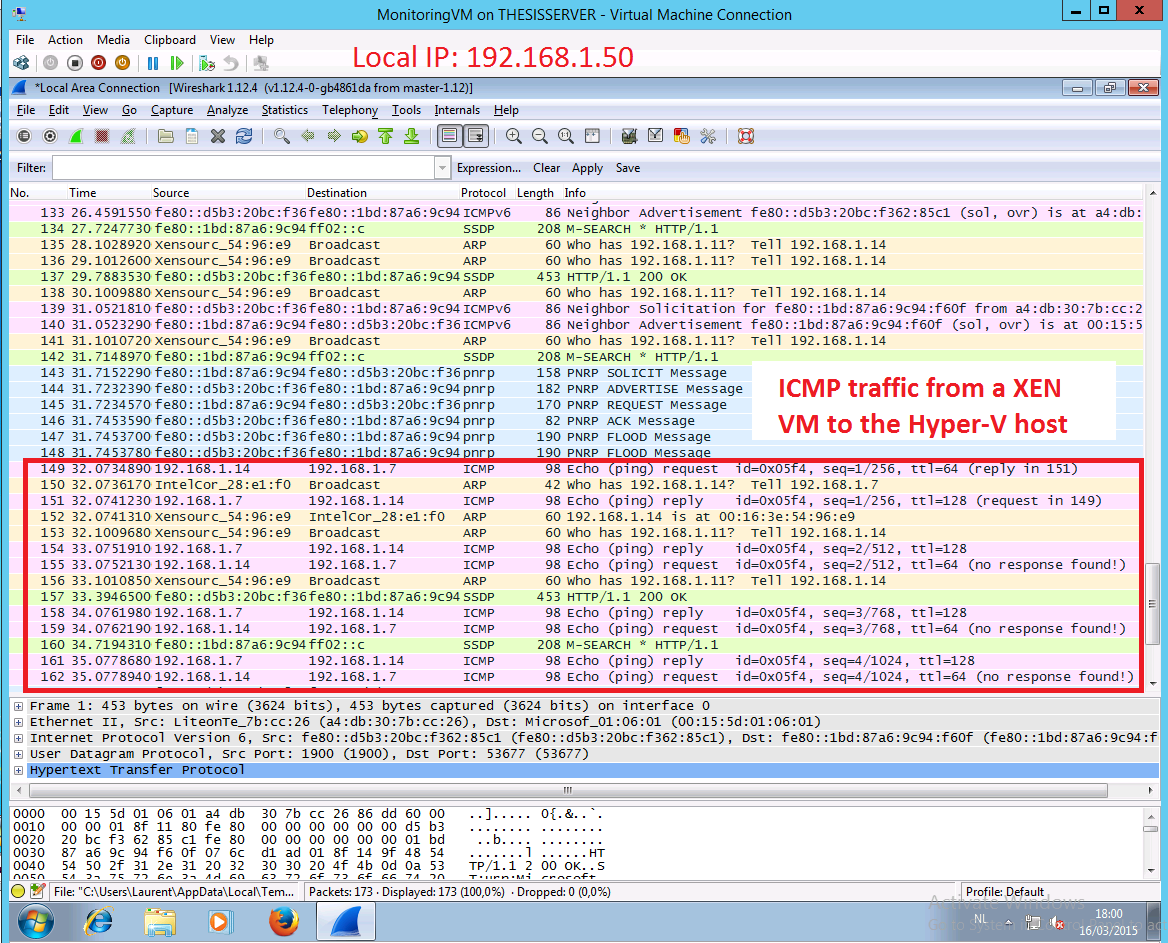
\includegraphics[width=\textwidth]{HyperV_12.png}
    \captionof{figure}{ICMP Ping traffic captured from a Xen VM to the Hyper-V host.}
\label{fig:network}
\end{minipage}
$\;$ \\ \\
Traffic capturing capabilities has been demonstrated with various configurations:
\begin{itemize}
\item Inter-VM between two Hyper-V VM's.
\item From a Xen VM to the Hyper-V host.
\item From a Xen VM to a Hyper-V VM.
\item From a Hyper-V VM to the Hyper-V host.
\end{itemize}
As illustrated, it is perfectly possible for an intruder to snif network traffic between VM's. Now that has the possibilities of packet sniffing / capturing has been shown, an important question raises: how can one prevent packet sniffing on virtual NIC's?



\subsection{Penetration testing on virtual networks}

Now that the possibilities of packet sniffing on virtual networks have been proven, it is time to perform some penetration testing on these virtual networks. Since packet sniffing is possible, we should be able to run an intrusion detection system (IDS) on either virtual network to intercept and prevent those penetration attacks. For this purpose, the Snort IDS will be used. \\ \\
The upcoming sections will provide the reader a brief description of the Snort IDS and its components as well as an overview of installing Snort. Next, the actual penetration testing, countermeasures and techniques to prevent certain types of network attacks will be discussed. 

\subsubsection{Snort}

Based on the different types of classifications of intrusion detection systems, one could classify Snort as a ``Signature-based Network Intrusion Detection and Prevention System''. \\

Additionally, Snort is open-source and capable of performing real-time network traffic analysis, as well as packet logging on IP networks. It consists of two major parts: the detection engine and the rules that are used to describe traffic that has to be collected or blocked. Furthermore, there exist two types of rules: rules that are available to all users (the so-called ``Community Rules'') and private, proprietary (paid) rules that are developed by SourceFire, the company behind Snort \citep{SnortLicense}. Addionally, so-called ``Registered rules'' are also available and are situated between the GPL rules and the proprietary rules. \\

I will make use of the freely available community rules combined with the ``Registered rules''. As one will notice, it will turn out that these rules are rather basic and need to be extende as well as additional rules have to be added in order to make Snort a viable IDS. This is allowed, since Snort uses the GPL license and we will make extensive use of this privilege to freely modify the rules. As previously mentioned, ``Registered rules'' have also been included in addition to the basic GPL rules. In order to do so, an account on the Snort website has been made and the rules were downloaded using \texttt{wget}. \\ 

As mentioned in the above paragraphs, Snort uses pre-defined rules to detect malicious activity on the network. One could compare it with the way antivirus programs work: any traffic that Snort picks up is matched against the database of rules and when a match has been found, an alert is raised.

\subsubsection{Preprocessors}

Preprocessors extend the functionality of Snort by examining packets or by modifying them so that Snort can properly interpret the packets. \citep{Preprocessor1}.

Some attacks cannot be detected by normal signatures (rules), so ``examine'' preprocessors detect suspicious behaviour. So one could say this type of preprocessor is used to detect non-signature-based attacks \citep{Preprocessor1}. 

The othe type of preprocessor is used to normalize traffic, so that Snort can match signatures in an accurate way.\\ \\
Preprocessor code is run before the detection engine is called. Additionally, each packet captured by Snort is cycled through every preprocessor, in order to discover even more attacks \citep{Preprocessor2}.

\subsubsection{PulledPork}

PulledPork (PP) is Perl script that will automatically download new Snort rules (signatures) in the background. Of course, one can always run PP directly at the command line to force the downloading of new rules \citep{PP}.

The downloaded rules are stored in a file called ``download.rules''.

\subsubsection{Barnyard2}

Barnyard2 is an interpreter for Snort binary output files. It is available under the GPL license and therefore, free to use \citep{Barnyard1}.

Barnyard2 allows Snort to write data to the disk in an efficient way. The parsing of binary data into different formats is handed over to a seperate process. Because Barnyard2 takes away some work, Snort will not miss any network traffic \citep{Barnyard2}.

\subsubsection{Packet capturing}

Packet capturing is accomplished by a program called \texttt{netsniff-ng}. Via a network interface set to promiscious mode, netsniff-ng captures all the traffic the sensors (explained later) of Ubuntu see and store as much of the information as possible. I.e., until the hard drive is full. Of course, a build-in mechanism to purge old data when the amount of data reaches a pre-defined level existss.

One could compare packet capturing with a video camera, that precisely sees and registers who, when and where was. The video camera is netsniff-ng and the persons walking around are the packets. All this is registered in a database.

Additionally, a video camera is also capable of registering of what people took with them. This is also the case with packet capturing: the payload of the packets can be examined as well as the destination address of the packets.

\subsubsection{NIDS and HIDS}

Network-based (NIDS) and host-based intrusion detection systems (HIDS) analyse the traffic that netsniff-ng captures and will log any malicious packets as well as sending alerts. There exist multiple IDSs:\\
\textbf{NIDS}
\begin{itemize}
\item Signature-based NIDS: Snort or Suricata. In this paper, Snort will be used.
\item Anomaly-based NIDS: Bro IDS. The definition of anomaly-based IDSs has been covered in the previous chapters and since Snort will be used, we will not dive deeper into Bro.
\end{itemize}
\textbf{HIDS}
\begin{itemize}
\item OSSEC: an open-source HIDS for Windows, Linux and Mac OS X. Instead of monitoring an entire network, OSSEC monitores only one specific host on suspicious activity \citep{OSSEC}.
\end{itemize}

\subsubsection{Analysis tools}

With Snort / Suricata data and the packet capturing of \texttt{netsniff-ng}, there is a vast amount of data available for the analist. To help managing the alerts generated by Snort or Suricata, some handy tools have been installed, including:

\begin{itemize}
\item \textbf{Sguil}: a network security analysis tool providing an intuitive GUI that provides access to realtime events and raw packet capturing data. The client is written in tcl/tk. In the client, one can view alerts of Snort, Bro, Suricata and OSSEC \citep{Sguil}.

The alerts are stored in a seperate MySQL database and this allows a user to query alerts by type, IP address or port, for example.

With Sguil, it is also possible to categorize alerts. This can be done either manually or automatically. The next chapter will provide more details of how this can be achieved \citep{Sguil}.

\item \textbf{Squert}: a web application that is used to view and query event data for the Sguil database. One could see it as a web interface for the Sguil database. It is neither ment to be a real-time interface, nor a replacement for Sguil, but more to bring additional visualization options to Sguil \citep{Squert}.

\item \textbf{Snorby}: a RoR (Ruby On Rails) web application that allows one to visualize Snort and Suricata alerts as well as perform queries on them. For example, listing the most active IDS signatures, most active sensors, \ldots. While all this can also be done with the Sguil database, Snorby offers a web interface instead of manually querying the Sguil database. In contrast to Sguil and Squert, Snorby uses his own, seperate database \citep{Snorby}.
\end{itemize}

\subsubsection{Running Snort IDS on a virtual network}

With Snort, Snorby and Sguil installed and configured, we can start using it. Of course, in order to be sure whether Snort indeed picks up all the traffic that flows through the network, we must first test it. The figure below illustrates the correct installation of Snort.
$\;$ \\ \\
\noindent\begin{minipage}{\textwidth}
    \centering
    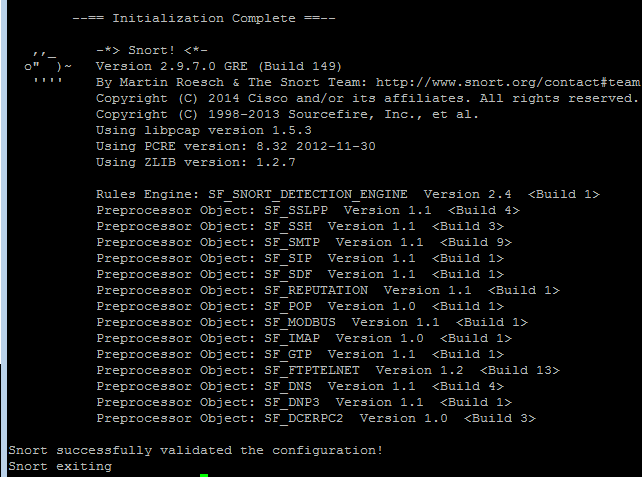
\includegraphics[width=0.8\textwidth]{Snort.jpg}
    \captionof{figure}{Confirmation of the correct installation of Snort.}
\label{fig:network}
\end{minipage}

\subsubsection{First things first: basic configuration of Snort}

First of all, we need to verify the network settings. Therefore, the \texttt{ifconfig} command is run. In addition, we also have a look at  \texttt{/etc/network/interfaces} to confirm the settings.
$\;$ \\ \\
\noindent\begin{minipage}{\textwidth}
    \centering
    \includegraphics[width=0.8\textwidth]{VM_network.png}
    \captionof{figure}{The sniffing / capturing interface \texttt{eth1} runs in promiscious mode and captures all the packets on the network. No IP address has been set (as it should be).}
\label{fig:network}
\end{minipage}
$\;$ \\ \\
\noindent\begin{minipage}{\textwidth}
    \centering
    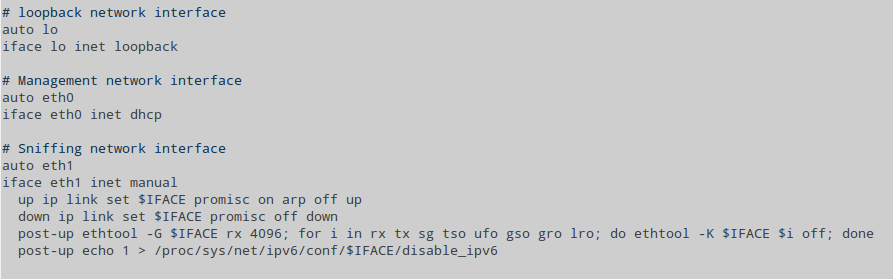
\includegraphics[width=\textwidth]{VM_network_3.png}
    \captionof{figure}{Confirmation of the network settings.}
\label{fig:network}
\end{minipage}
$\;$ \\ \\
After having verified that the network settings are correct, we can configure some of the basic options of Snort. This includes network settings and is performed in ``snort.conf''. For example, the network segments on which Snort has to listen have to be configured.
$\;$ \\ \\
\noindent\begin{minipage}{\textwidth}
    \centering
    \includegraphics[width=0.8\textwidth]{VM_network_2.png}
    \captionof{figure}{We are working on the 192.168.1.0/24 network, but by means of testing, we have setup Snort to listen on the /16 subnet (255.255.0.0). As it will turn out, this will \textbf{not} affect the correct working of Snort. So one could randomly choose a value (8, 16 or 24).}
\label{fig:network}
\end{minipage}

\subsubsection{Configuring Snort rules}
\label{subsec:rules}
Throughout this paper, we will frequently modify and add Snort rules (signatures), so an explanation of how a Snort rule is composed is given first. \\ \\
Most Snort rules are written in a single line. When a rules needs to span multiple lines, this can always be performed by adding a backslash ($\backslash$) at the end of the line.

Snort rules consist of two main parts: the rule header and multiple rule options. The header contains the rule's action method, protocol, source IP, source port, destination IP and destination port.

The rule options contains alert messages, signature ids, revisions and many more options. \\ \\
Below is the general layout of a Snort rule. \\ \\
\textbf{action protocol sourceIP sourcePort $\rightarrow$ destinationIP destinationPort (OPTIONS);} \\ \\
To clear things up, an example is provided. \\
Consider following rule:

\textbf{alert icmp any any $\rightarrow$ any any (msg:``ICMP ping"; sid:100002;)} \\ \\
This could be read as follows: ``alert all ICMP traffic from any source IP, from any port to any destination IP and to any destination port. Alert as ``ICMP ping'' and the unique id of the rule is 100002.''. \\ \\
Action can be one the following \citep{SnortRules}:
\begin{itemize}
\item alert: an alert is generated after which the packet is logged.
\item log: just log the packet, do not generate any alerts.
\item pass: ignore the packet.
\item drop: log and block the packet.
\item reject: log and block the packet and sent a TCP reset or ICMP port unreachable when TCP or UDP is used, respectively.
\end{itemize}
Protocol can be one the following \citep{SnortRules}:
\begin{itemize}
\item TCP
\item UDP
\item ICMP
\item IP
\end{itemize}
The IP address can be an ordinary IP address or an address/CIDR combination. For example, 192.168.1.0/24 would mean the block of addresses from 192.168.1.1 till 192.168.1.254.

\subsubsection{Updating the rules using PulledPork}

After installing Snort, it is a good practise to update the ruleset, just as one may do when one has just installed an antivirus program. This is done using the \texttt{update-rules} command.

One could make a cron-job of this command to run it, for example, every day at 3 am.
$\;$ \\ \\
\noindent\begin{minipage}{\textwidth}
    \centering
    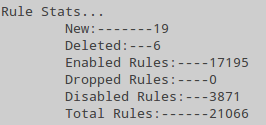
\includegraphics{VM_Pulledport_rules.png}
    \captionof{figure}{After PulledPort has run, one can notice that 19 new rules have been downloaded and added to the ruleset of Snort.}
\label{fig:network}
\end{minipage}

\subsubsection{Confirming that Snort is actually working}

To confirm that all the agents (sensors) and the servers are running, the following command is executed: \texttt{sostat -quick}. Which yields following output:
$\;$ \\ \\
\noindent\begin{minipage}{\textwidth}
    \centering
    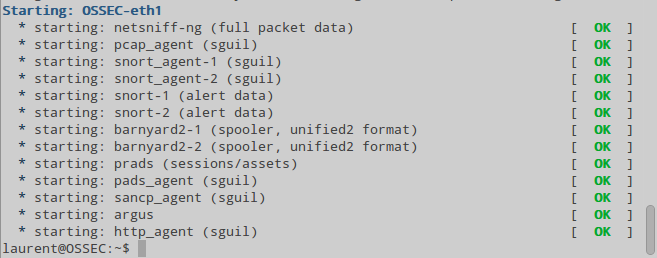
\includegraphics[width=\textwidth]{VM_OK.png}
    \captionof{figure}{Everything is running fine.}
\label{fig:network}
\end{minipage}
$\;$ \\ \\
However, we cannot assume that, just by installing and configuring Snort - where everything \textbf{seems} to be working, that everything \textbf{is} actually working. To convince myself, a simple Snort rule has been made to detect and alert for any ICMP Ping traffic on the network: \\

\textbf{alert icmp any any $\rightarrow$ any any (msg:``ICMP Ping traffic"; sid:100002;)} \\ \\
When pinging from the attack machine to the victim, Snort indeed picks up the ICMP traffic and fires a corresponding alert, as well as storing the information in the database. This can be seen in the figure below.
$\;$ \\ \\
\noindent\begin{minipage}{\textwidth}
    \centering
    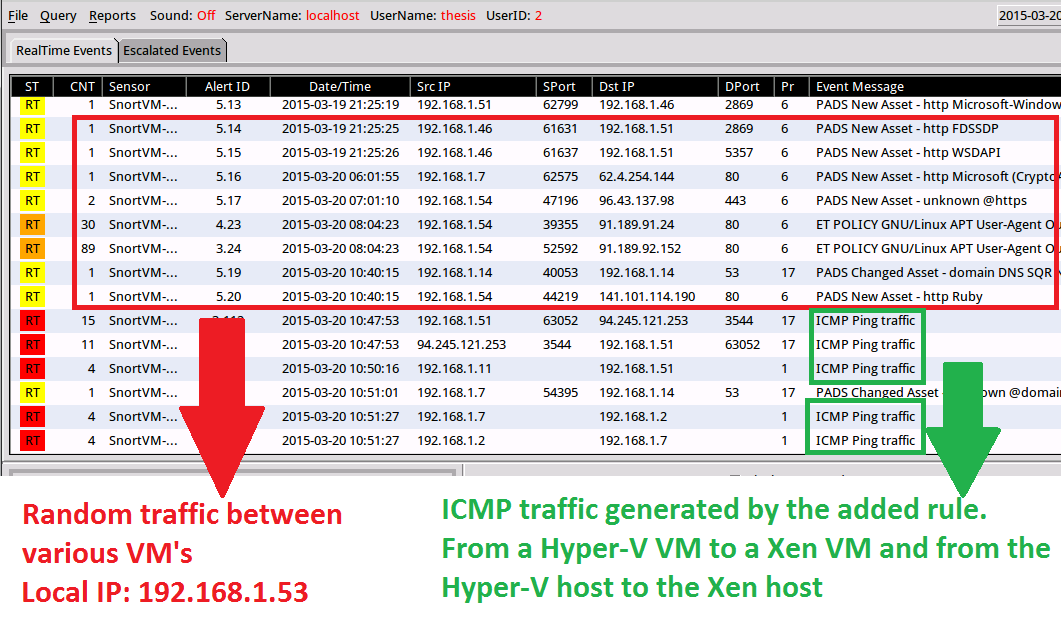
\includegraphics[width=\textwidth]{Snort_3_2.png}
    \captionof{figure}{Ping traffic gets picked up by Snort.}
\label{fig:network}
\end{minipage}
$\;$ \\ \\
This can also be confirmed by executing \texttt{tcpdump} on the Snort VM:
$\;$ \\ \\
\noindent\begin{minipage}{\textwidth}
    \centering
    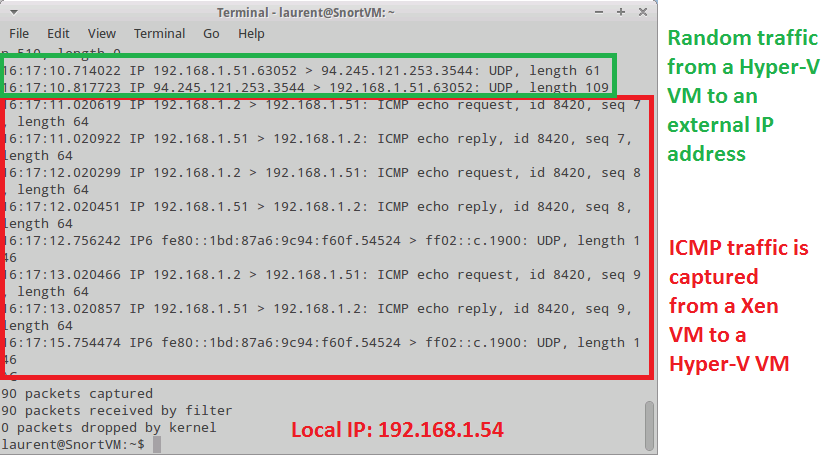
\includegraphics[width=\textwidth]{Snort_1.png}
    \captionof{figure}{\texttt{tcpdump} confirms that the Snort VM is receiving traffic other than the traffic destinated for the VM. This proves the fact that the Snort VM is actually sniffing traffic.}
\label{fig:network}
\end{minipage}
$\;$ \\ \\
However, Snort is only picking up intrusions on the Hyper-V network including the Hyper-V host. Thus, intrusions on the Xen virtual network are not detected, because those VM's resides on a seperate virtual switch. \\

So I wanted a way to also detect malicious activity on the Hyper-V network with the SnortVM running on a seperate virtual network. \\

Since I'm using in-kernel bridging for the virtual Xen switch, my initial idea was to snif the bridged interface (since all traffic - also between VM's - passes through this interface) and copy all the packets to another, physical interface set in promiscious mode. From there, I could then forward the packets to the Hyper-V network. \\ \\
However, it is not possible to forward packets on an interface that is in promiscious mode. So instead of making a copy of the bridged interface, the only solution was to make a copy of the packets on each virtual interface connected to the vSwitch.

This solution works fine as illustrated in the following screenshots.
$\;$ \\ \\
\noindent\begin{minipage}{\textwidth}
    \centering
    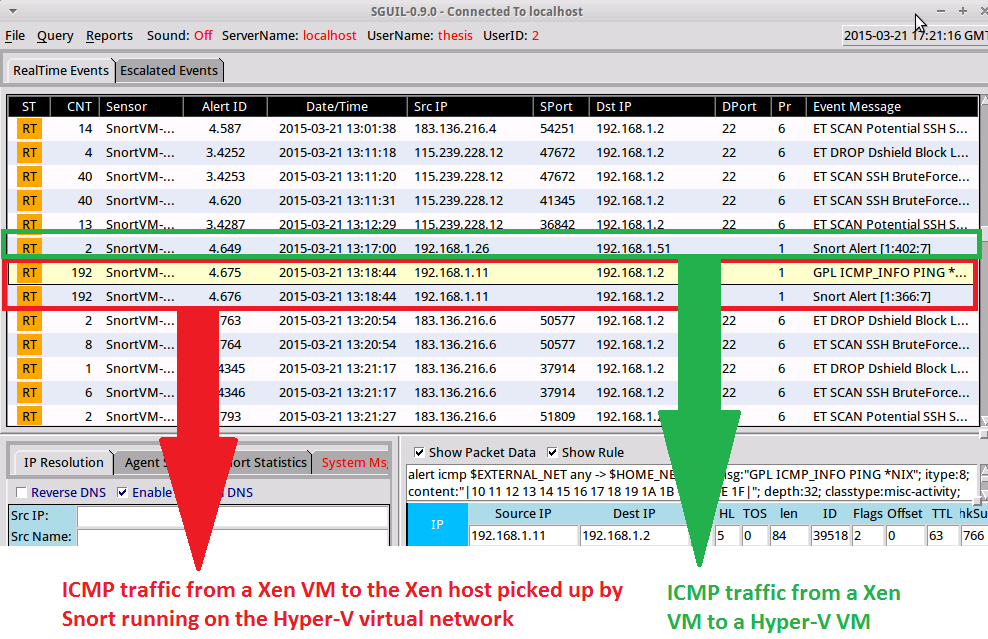
\includegraphics[width=\textwidth]{Snort_4.png}
    \captionof{figure}{Traffic originating from a Xen VM to the Xen host is captured by the Snort VM as well as traffic originating from a Xen VM to a Hyper-V VM.}
\label{fig:network}
\end{minipage}
$\;$ \\ \\
\noindent\begin{minipage}{\textwidth}
    \centering
    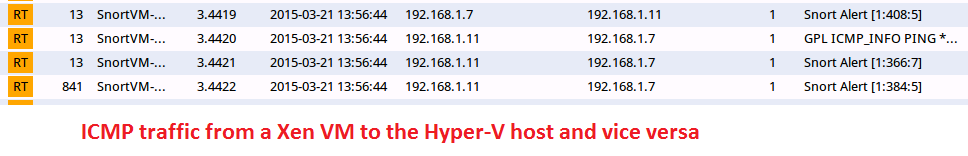
\includegraphics[width=\textwidth]{Snort_5.png}
    \captionof{figure}{Traffic from the Hyper-V host (the hypervisor where the Snort VM is installed on) to a Xen VM is captured by Snort.}
\label{fig:network}
\end{minipage}
$\;$ \\ \\
\noindent\begin{minipage}{\textwidth}
    \centering
    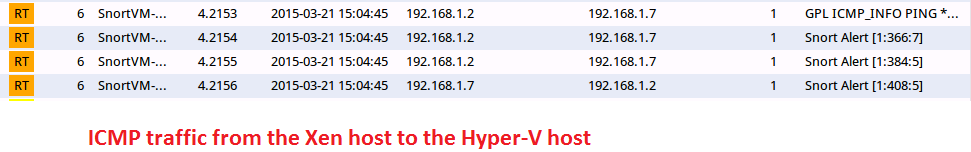
\includegraphics[width=\textwidth]{Snort_6.png}
    \captionof{figure}{Traffic between the two hypervisors is picked up as well.}
\label{fig:network}
\end{minipage}
$\;$ \\ \\
\noindent\begin{minipage}{\textwidth}
    \centering
    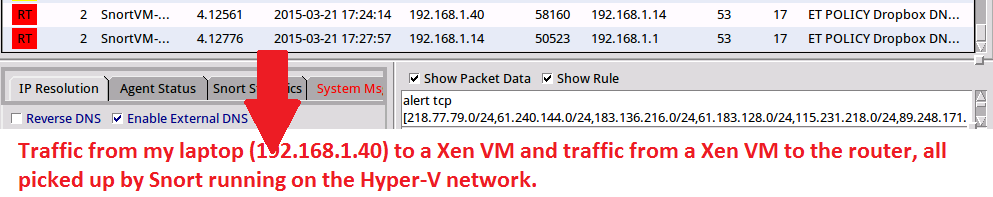
\includegraphics[width=\textwidth]{Snort_17.png}
    \captionof{figure}{Traffic originating from outside either virtual network to any virtual network and traffic destinated to a target outside any virtual network is detected by Snort.}
\label{fig:network}
\end{minipage}
$\;$ \\ \\
\noindent\begin{minipage}{\textwidth}
    \centering
    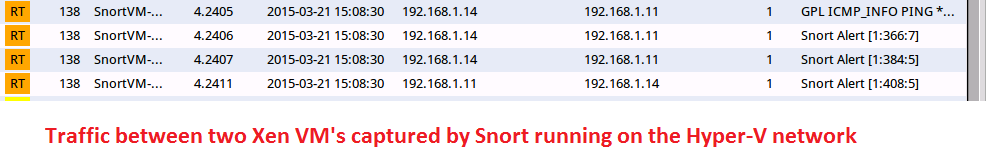
\includegraphics[width=\textwidth]{Snort_8.png}
    \captionof{figure}{Internal traffic between Xen VM's is intercepted by Snort.}
\label{fig:network}
\end{minipage}
$\;$ \\ \\
\textbf{So to summarize, the following is possible / is achieved regarding intrusions:}
\begin{itemize}
\item Detecting intrusions between two VM's running on the Hyper-V virtual network.
\item Detecting intrusions between a VM running on the Hyper-V virtual network and the Xen virtual network and vice versa.
\item Detecting intrusions between two VM's running on the Xen virtual network.
\item Detecting intrusions between the Xen host and Hyper-V host and vice versa.
\end{itemize}

\subsection{Actual penetration testing}

In order to make sure that Snort is actually protecting our network against numerous and various anomalies, it is essential to test Snort against various attacks. Based on how Snort reacts on the attacks, we will configure Snort, that is, modifying the rules (signatures), add rules if no alerts are raised or removing some of the rules that are triggering false alerts. Not only can one adjust the rules, also thresholds and limitations of how many alerts each rule is allowed to generate can be set. \\ \\
Of course, false positives will also be generated and the art of configuring Snort is minimizing the amount of false positives and maximizing the generation of alerts of real threads.

\subsubsection{What types of attacks will be performed?}

Various types of network and host attacks will be executed on the network in order to test Snort's reaction. These types include:
\begin{itemize}
\item Port scans
	\begin{itemize}
	\item Basic port scan
	\item Advanced port scan
	\end{itemize}
\item Webserver attacks
	\begin{itemize}
	\item XSS
	\item SQL Injection
	\item Command Injection
	\end{itemize}
\item FTP server attacks
	\begin{itemize}
	\item FTP root access
	\item FTP malicious payloads
	\item Various other FTP attacks
	\end{itemize}
\item SSH attacks
\item Database attacks
	\begin{itemize}
	\item Database scanning
	\item Login attempts (including root access)
	\item Bruteforce attempts
	\end{itemize}
\item Trojan and virus injection / infection
\item DOS attacks
\end{itemize}

\subsubsection{Motivation for the choice of the attacks}

Why were these nine types of attacks chosen? The attacks are based on the actual services provided by some servers in my own home network. I have for example a web server running, an FTP server, a Samba server and a MySQL server. All those servers are running on Linux and to remotely login on those servers, SSH is frequently used.

So that is why webserver, FTP and SMB attacks will be performed. In addition, each hacker starts by scanning the network for running computers and once a computer has been found, a port scan is executed to scan the host for open ports which the hacker can exploit.

\subsubsection{Testing methods}

In order to avoid a too high level of artificial server setup, all the attacks are performed on production servers. Before doing so, the correct functioning of those services is controlled and when it is confirmed that the service / server that is about to be attacked functioning properly, the actual attack is performed.

After the attack has been performed, Sguil is checked for realtime events. Remember that Snort writes its ``findings'' to the Sguil database. When the attack is listed, it means that Snort has successfully picked up / recognized the attack

Also the DOS attack is performed on two production servers being the FTP server and the webserver. However, the Trojan infection is performed on my own laptop, not a real production server. So I will be infecting my own computer from a VM acting as the attacker.

\subsubsection{NMAP scanning}

Once the attacker knows which hosts are online, he can start querying a host to determine what services are running on the host or what types of protocols the host supports. This is the first phase in a network attack: the reconnaissance phase. 

That is why first of all, some NMAP scanning was performed for reconnaisance of open ports and running services of the target hosts. I started with an unfragmented scan on a Hyper-V VM from the webserver, which has NMAP installed.

\paragraph{Unfragmented packets}
First \ldots.
$\;$ \\ \\
\noindent\begin{minipage}{\textwidth}
    \centering
    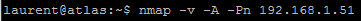
\includegraphics{Ping_Unfragmented_putty.png}
    \captionof{figure}{The NMAP command as executed on the webserver (atlas, 192.168.1.11).}
\end{minipage}
$\;$ \\ \\
\noindent\begin{minipage}{\textwidth}
    \centering
    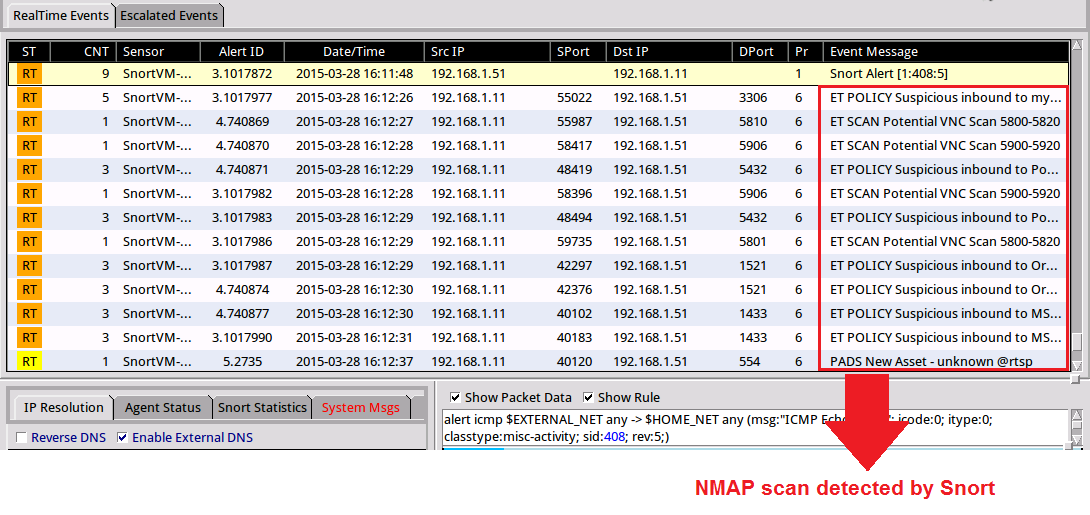
\includegraphics[width=\textwidth]{Ping_Unfragmented.png}
    \captionof{figure}{Basic, unfragmented NMAP scanning of a Hyper-V VM (192.168.1.51). The SnortVM has the IP address of 192.168.1.50. Snort reports each attempt to scan a particular port number.}
\end{minipage}
\paragraph{Fragmented SYN packets}
Next, I performed an NMAP scan with fragmented packets, which splits up the TCP header over several tiny packets to trick / fool IDSs and firewalls. This way, an attacker hopes to evade packet filters. \\ \\
The NMAP command executed is the following: \\ \\
\noindent\begin{minipage}{\textwidth}
    \centering
    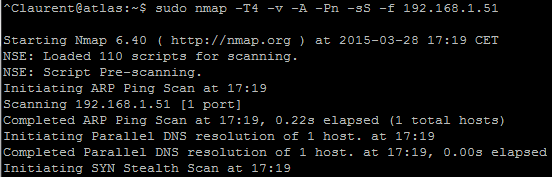
\includegraphics{Ping_Fragmented_2_putty.png}
    \captionof{figure}{The NMAP stealth, SYN packet command as executed on the webserver (atlas, 192.168.1.11).}
\end{minipage}
$\;$ \\ \\
The stealth, fragmented ICMP ping scan is not detected by Snort. However, Snort did detect the scan for running services as can be seen in the following figure. \\ \\
\noindent\begin{minipage}{\textwidth}
    \centering
    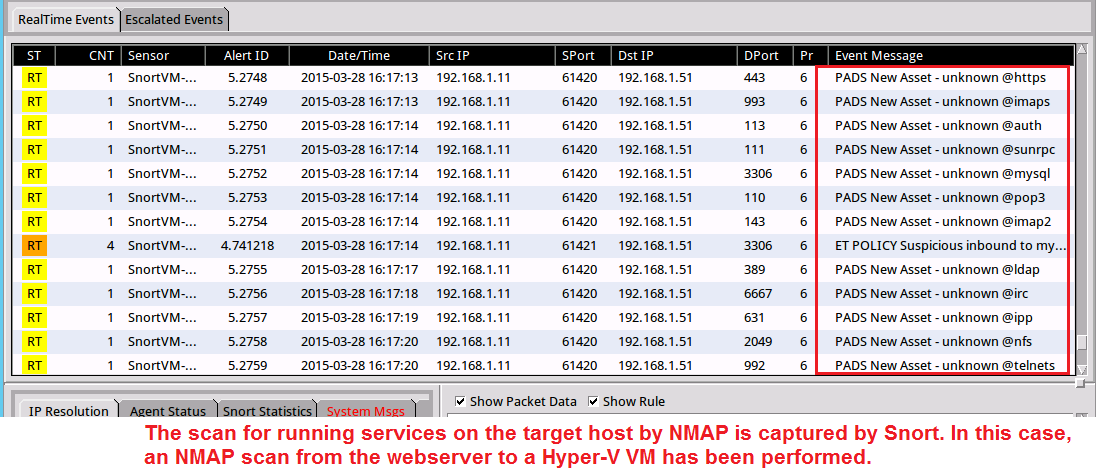
\includegraphics[width=\textwidth]{Ping_Fragmented.png}
    \captionof{figure}{The scan for running services from the stealth scan is detected by Snort.}
\end{minipage}
$\;$ \\ \\
\noindent\begin{minipage}{\textwidth}
    \centering
    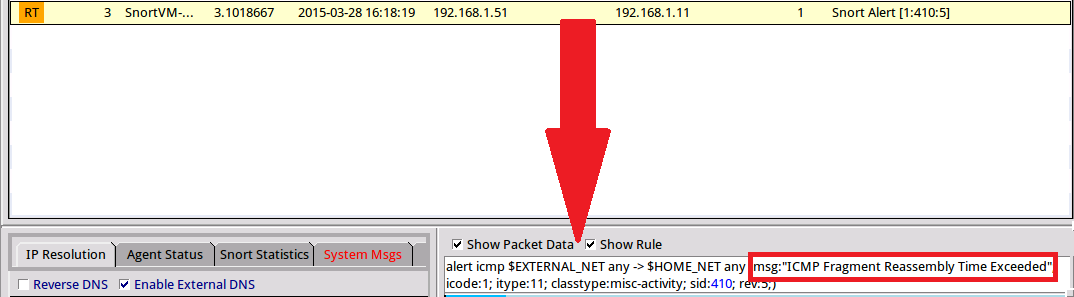
\includegraphics[width=\textwidth]{Ping_Fragmented_2.png}
    \captionof{figure}{However, this Snort alert indicates that a host reassembling a fragment datagram cannot complete the reassembly due to missing fragments whitin the time limit (60s by default). However, I'm not sure whether this is Snort warning for a fragmented / stealth scan.}
\end{minipage}
$\;$ \\ \\
Then I performed an ICMP ping to the Hyper-V VM (192.168.1.51) with a size of 1000 bytes. This gets detected by Snort right away. \\ \\
\noindent\begin{minipage}{\textwidth}
    \centering
    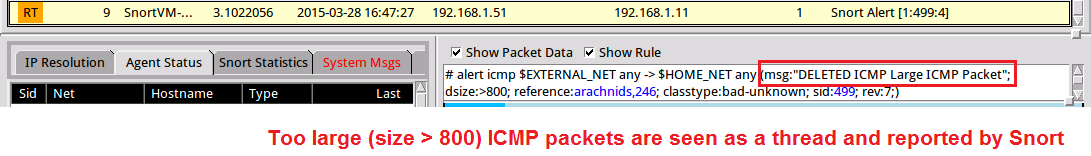
\includegraphics[width=\textwidth]{Ping_Large.png}
    \captionof{figure}{ICMP ping with large packet size is detected by Snort.}
\end{minipage}
$\;$ \\ \\
\noindent\begin{minipage}{\textwidth}
    \centering
    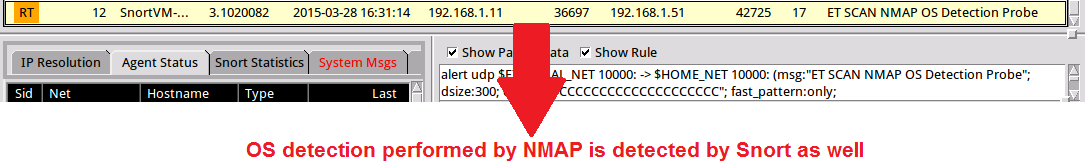
\includegraphics[width=\textwidth]{OS_Detection.png}
    \captionof{figure}{OS detection from a NMAP scan is also detected by Snort.}
\end{minipage}

\subsubsection{Preventing port scanning with Snort}

In section \ref{subsec:rules}, an overview of the different action types of Snort rules has been supplied. One of these actions is \texttt{drop}, which causes the matched packets to be blocked. Therefore, different network attacks including port scanning can be prevented.

As an example, consider the following rule: \\
\textbf{alert icmp any any $\rightarrow$ any any (msg:``ICMP ping"; sid:100002;)} \\
This rule will generate alerts when ICMP Ping packets are intercepted. However, when changing \texttt{alert} to \texttt{drop}, ICMP ping packets are filtered out of (from) the network and thus preventing port scanning. \\ \\
This process can be repeated for every rule that generated alerts. Of course, in order to improve security, one can also configure the firewall to restrict the effectivity of port scans. Most effective way to do so is denying all traffic and only allowing the traffic needed to access the internal services. Also, tracking malicious activity over time and configuring rules to cut off attacks when a treshold is reached. For example, when 50 consecutive ICMP Ping requests are detected.

\subsubsection{Webserver attacks}

This section will cover some common webserver attacks, such as XSS attacks, SQL injections and command injections.

\subsubsection{Cross-site scripting (XSS) attack}

Sometimes, one can abuse an URL of a webpage to inject JavaScript code into the page. This is called a cross-site scripting (XSS) vulnerability. If a hacker gives the modified URL to someone else and he can get this person to click on the modified links, a hacker / attacker can achieve the following: change the content of the page, steal cookie values, gain access to the user's history, \ldots. This is why we want to detect this. \\ \\
Therefore, I made a vulnerable PHP webpage myself, to exploit an XSS atack. The page takes the ``name'' parameter from the URL and displays it on the page. But this makes is ideal for an XSS attack.
$\;$ \\ \\
\noindent\begin{minipage}{\textwidth}
    \centering
    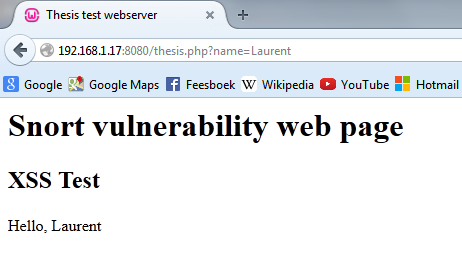
\includegraphics[width=0.8\textwidth]{VM_XSS_3_Better.png}
    \captionof{figure}{The vulnerable webpage before the attack. It displays the string value that is provided in the ``name'' parameter in the URL.}
\end{minipage}
$\;$ \\ \\
Then, the following script is injected into the page: \\
\textbf{$<$script$>$alert('XSS vulnerability')$<$/script$>$}. \\
Which yields following output:
$\;$ \\ \\
\noindent\begin{minipage}{\textwidth}
    \centering
    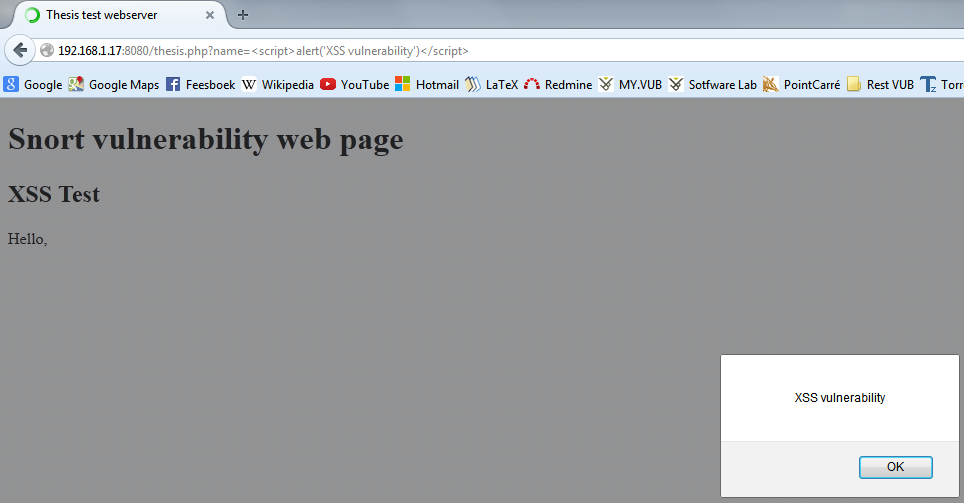
\includegraphics[width=\textwidth]{VM_XSS_2_Better.png}
    \captionof{figure}{The script in action\ldots.}
\end{minipage}
$\;$ \\ \\
As one can observe, the script is indeed successfully injected into the webpage.
$\;$ \\ \\
\noindent\begin{minipage}{\textwidth}
    \centering
    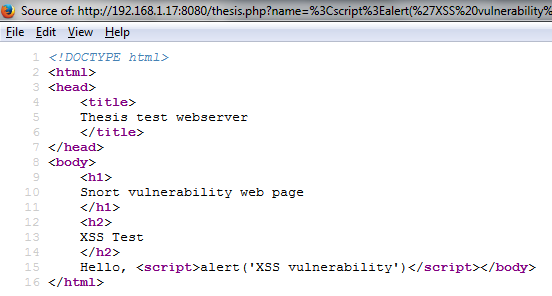
\includegraphics[width=\textwidth]{VM_XSS_1_Better.png}
    \captionof{figure}{The script is successfully injected into the PHP page.}
\end{minipage}
$\;$ \\ \\
How did Snort react? Snort detects this anomaly right away, without the need for adding extra rules, as can be seen in the following screenshot. However, one can also avoid this attack from happening by changing the ``action'' method in the rule from ``alert'' to ``drop''.
$\;$ \\ \\
\noindent\begin{minipage}{\textwidth}
    \centering
    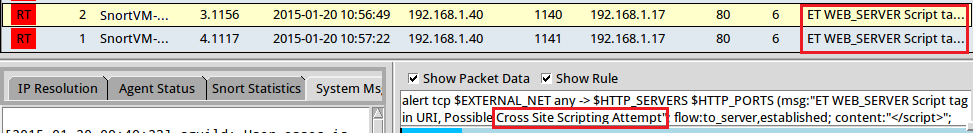
\includegraphics[width=\textwidth]{VM_XSS_5.png}
    \captionof{figure}{Fortunately, Snort detects the XSS attack without the need for adding additional rules.}
\end{minipage}
$\;$ \\ \\
\noindent\begin{minipage}{\textwidth}
    \centering
    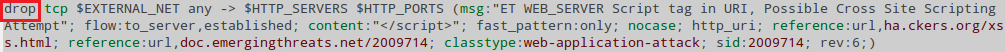
\includegraphics[width=\textwidth]{VM_XSS_6.png}
    \captionof{figure}{To prevent XSS attacks from happening, one can change ``alert'' to ``drop'' in the rules that triggers the alert.}
\end{minipage}

\subsubsection{SQL Injection}

SQL Injection is an attack technique in which users can insert SQL commands as strings that are passed to an SQL server, via a webpage input \citep{SQLInj}. It can be used to read sensitive data from a database or to perform administrative tasks to the database, for example: shutting down the DBMS. \\ \\
To detect such attacks, a custom PHP webpage has been created that is vulnerable to an SQL injection attack. \\ \\
To provide the reader a general overview, the entire content of the MySQL ``Persons'' table is displayed on the webpage. Obviously, in reality, nothing is displayed when a user first loads the page. But the content is displayed for information purposes.
$\;$ \\ \\
\noindent\begin{minipage}{\textwidth}
    \centering
    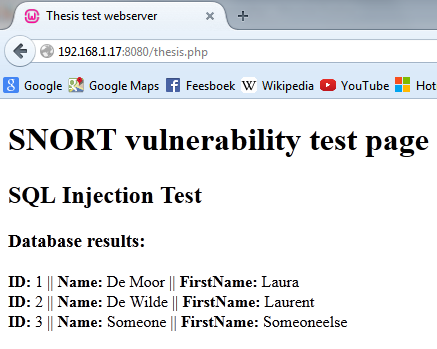
\includegraphics{VM_SQL_1.png}
    \captionof{figure}{Persons table in the test database running on MySQL 5.6 populated with 3 records.}
\end{minipage}
$\;$ \\ \\
Then, an input textfield is created where the user can enter the firstname of a person he is looking for. The source code is listed below:
$\;$ \\ \\
\noindent\begin{minipage}{\textwidth}
    \centering
    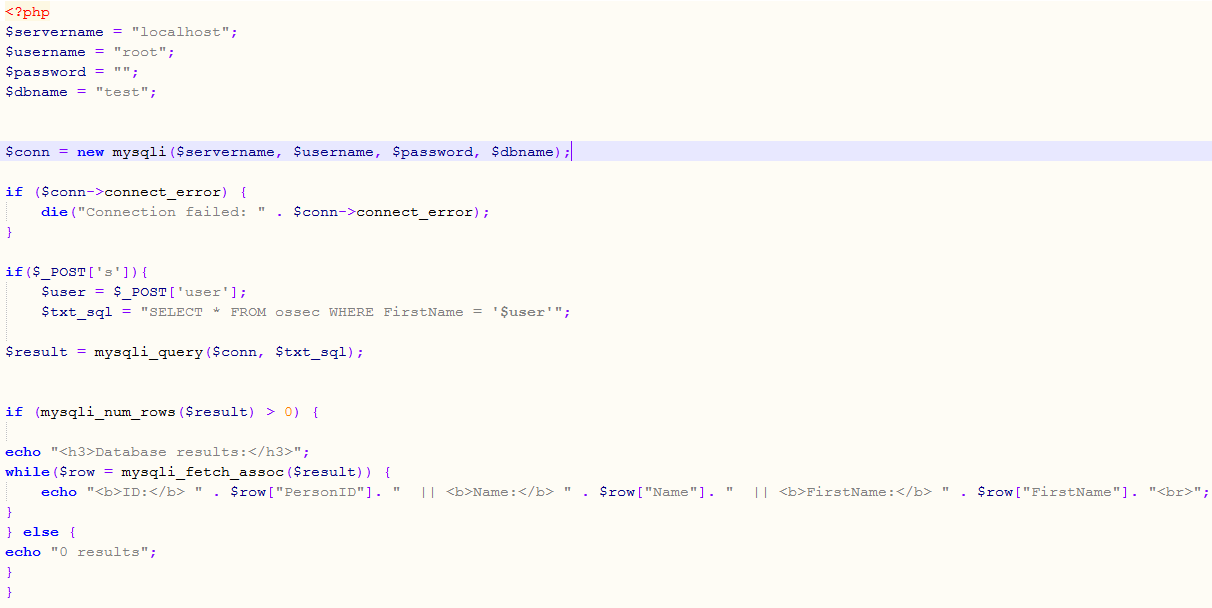
\includegraphics[width=\textwidth]{VM_SQL_3.png}
    \captionof{figure}{Persons table in the test database running on MySQL 5.6 populated with 3 records.}
\end{minipage}
$\;$ \\ \\
The next screenshot shows an example of how a POST request can look like. In this example, the user has entered the search string ``Laurent".
$\;$ \\ \\
\noindent\begin{minipage}{\textwidth}
    \centering
    \includegraphics[width=\textwidth]{VM_SQL_2.png}
    \captionof{figure}{Persons table in the test database running on MySQL 5.6 populated with 3 records.}
\end{minipage}
$\;$ \\ \\
Of course, when the textfield is empty and the query is submitted, nothing is displayed. But when an attacker enters the string ``OR $1=1$'', he gets to see all the information stored in the Persons table. This is called SQL injection based on $1=1$ is always true. It is an attempt to make a query succeed no matter what.
$\;$ \\ \\
\noindent\begin{minipage}{\textwidth}
    \centering
    \includegraphics{VM_SQL_4.png}
    \captionof{figure}{SQL injection attack in action with all the results displayed on the webpage.}
\end{minipage}
$\;$ \\ \\
And did Snort react on this type of webserver attack? Yes it did, as can be seen in the following screenshots:
$\;$ \\ \\
\noindent\begin{minipage}{\textwidth}
    \centering
    \includegraphics[width=\textwidth]{VM_SQL_8.png}
    \captionof{figure}{Snort alerts for a possible SQL injection.}
\end{minipage}
$\;$ \\ \\
\noindent\begin{minipage}{\textwidth}
    \centering
    \includegraphics[width=\textwidth]{VM_SQL_9.png}
    \captionof{figure}{The triggering rule. Once again, one could change ``alert'' to ``drop'' in order to prevent the SQL injection from happening.}
\end{minipage}

\subsubsection{Command injection}

A command injection attack is an attack in which a hacker tries to execute commands on the host operating system using a vulnerable (web)application. \\ \\
To simulate this attack, I created a vulnerable PHP webpage that returns the content of a file that the user requested. It does this by executing the ``type'' command on the host machine. But as one may have guessed, an attacker can also execute a command this way.  \\ \\
Following screenshot displays the source code of the webpage.$\;$ \\ \\
\noindent\begin{minipage}{\textwidth}
    \centering
    \includegraphics[width=\textwidth]{VM_Command_2.png}
    \captionof{figure}{The source code of the webpage. Note the ``shell\_exec'' statement.}
\end{minipage}
$\;$ \\ \\
An actual example of command injection is listed below. Here, the ``ipconfig'' command is executed on the target host and all information about the network interfaces is returned.
$\;$ \\ \\
\noindent\begin{minipage}{\textwidth}
    \centering
    \includegraphics[width=\textwidth]{VM_Command_1.png}
    \captionof{figure}{A command injection attack has just been launched and the results of executing the \texttt{ipconfig /all} command are displayed on the webpage.}
\end{minipage}
$\;$ \\ \\
Another example is provided below: when supplying the \texttt{netstat} command to the URL, an intruder can also obtain information about which ports are currently opened.
$\;$ \\ \\
\noindent\begin{minipage}{\textwidth}
    \centering
    \includegraphics[width=\textwidth]{VM_Command_4.png}
    \captionof{figure}{Output of the \texttt{netstat -a} command displayed on the web page.}
\end{minipage}
$\;$ \\ \\
How did Snort react on this thread? Well, at first, i did NOT. Meaning that there are some extra rules needed.
Especially, we want to look for executable files that are passed in the URL, because an attackers usually wants to execute programs (commands) on the host machine. However, it turned out that Snort actually already had a rule that alerts for this kind of attack, but it turned out this rule had been disabled. So enabling the rule was sufficient to make Snort alert on command injection attacks.
$\;$ \\ \\
\noindent\begin{minipage}{\textwidth}
    \centering
    \includegraphics[width=\textwidth]{VM_Command_3.png}
    \captionof{figure}{Snort alerting for command injections.}
\end{minipage}
$\;$ \\ \\
Again, changing the action from \texttt{alert} to \texttt{drop} will cause Snort to block these packets and thus preventing this command injection from happening.

\subsubsection{FTP server attacks}

Next, some attacks on the FTP server \texttt{vsftpd} running on a Xen virtual network are executed to see how Snort reacts on this. The FTP server has IP address 192.168.1.16 and runs on a Xen VM called ``farbauti''. The client computer has the IP address 192.168.1.40 and runs a Windows 7 Professional 64 edition. All FTP attacks were launched using FileZilla Client 3.10. \\
The following will be tested: attempting to login as root user and attempting to attack the FTP server with various attack methods, e.g.: command overflow, format string, \ldots. With a \textbf{command overflow}, a cracker sents overly long commands to the FTP server (that is, with a high amout of buffer content). This leaves the hacker the opportunity to execute code on the FTP server. \\
When the \textbf{\texttt{printf-style} format specifier} is sent as argument to some FTP commands, it causes data on the stack to be overwritten. This is because the FTP server trying to process data containing such format strings, eventually resulting in the possibility to execute code on the FTP server. \\
Remember that the Snort VM runs on the Hyper-V network and has IP address of 192.168.1.50. \\ \\
\noindent\begin{minipage}{\textwidth}
    \centering
    \includegraphics[width=\textwidth]{FTP_1.png}
    \captionof{figure}{First, I created a rule to actually detect FTP traffic as I plan to DOS attack the FTP server is a later stage. The starting of the FTP service and some FTP traffic are detected by Snort.}
\end{minipage}
$\;$ \\ \\
\noindent\begin{minipage}{\textwidth}
    \centering
    \includegraphics[width=\textwidth]{FTP_2.png}
    \captionof{figure}{Successful FTP logins are also detected by Snort (however, this is not a thread and can be disabled by simply comment the rule that triggered the alert.}
\end{minipage}
$\;$ \\ \\
\noindent\begin{minipage}{\textwidth}
    \centering
    \includegraphics[width=\textwidth]{FTP_4.png}
    \captionof{figure}{Attempting to login as root.}
\end{minipage}
$\;$ \\ \\
\noindent\begin{minipage}{\textwidth}
    \centering
    \includegraphics[width=\textwidth]{FTP_3.png}
 \captionof{figure}{FTP root access is successfully detected.}
\end{minipage}
$\;$ \\ \\
For the actual FTP server attacks, I used Metasploit's db\_autopwn command on port 21 on target host 192.168.1.16. \\ \\
\noindent\begin{minipage}{\textwidth}
    \centering
    \includegraphics[width=\textwidth]{FTP_6.png}
 \captionof{figure}{The command to attack the FTP server as seen in Metasploit.}
\end{minipage}
$\;$ \\ \\
\noindent\begin{minipage}{\textwidth}
    \centering
    \includegraphics[width=\textwidth]{FTP_5.png}
 \captionof{figure}{Snort reported the various attacks.}
\end{minipage}

\subsubsection{Preventing FTP server attacks}

Some early versions of ProFTPd are vulnerable to command overflow attempts, so installing the latest software - and security updates of the installed FTP server is the first step in denying hackers taking over control of the system. One might also consider moving on onto more secure FTP servers such as \texttt{vsftpd}. While peforming the attack using Metasploit, the \texttt{vsftpd} server did not go offline, nor did the penetration attempts such as command overflow attempts succeeded.

\subsubsection{SSH attacks}

There was no need to simulate an SSH attack, as the next screen capture reveals: \\ \\
\noindent\begin{minipage}{\textwidth}
    \centering
    \includegraphics[width=\textwidth]{SSH.png}
 \captionof{figure}{Appearantly, someone tried to SSH scan my Xen server\ldots. This was fortunately detected by Snort.}
\end{minipage}
$\;$ \\ \\
How can SSH attacks be prevented?
\begin{itemize}
\item Allow only one IP address to be connected to the SSH server.
\item Run the SSH daemon on a non-standard port.
\item Make use of \texttt{hosts.allow} and \texttt{hosts.deny} to allow only certain IP addresses to connect to the server via SSH.
\end{itemize}
$\;$ \\ \\
\noindent\begin{minipage}{\textwidth}
    \centering
    \includegraphics[width=\textwidth]{Hosts_Allow.png}
 \captionof{figure}{An example of \texttt{hosts.allow}. In this example, only computer with IP address of 192.168.1.2 and 192.168.1.2 are allowed to connect to the server through SSH.}
\end{minipage}
$\;$ \\ \\
\noindent\begin{minipage}{\textwidth}
    \centering
    \includegraphics[width=\textwidth]{Hosts_Deny.png}
 \captionof{figure}{An example of \texttt{hosts.deny}. This file is used in combination with \texttt{hosts.allow} and indicates that only IP addresses of 192.168.1.2 and 192.168.1.40 are allowed to connect to the server through SSH and that all other IP addresses have their access denied.}
\end{minipage}
\begin{itemize}
\item Use \texttt{hashlimit} in \texttt{iptables} to, for example, allow only one SSH connection per IP address per minute.
\end{itemize}

\subsubsection{Database server attacks}

A scan looking for MySQL databases on the network has been executed, as well as commands to show the available databases on the server and root login.

For the database scan,  Metasploit has been used again. The IP address of the MySQL server is 192.168.1.23 and the MySQL database runs on a Xen VM called \texttt{mimas}. \\ \\
\noindent\begin{minipage}{\textwidth}
    \centering
    \includegraphics[width=\textwidth]{MySQL_3.png}
 \captionof{figure}{Metasploit is scanning the network for databases...}
\end{minipage}
$\;$ \\ \\
\noindent\begin{minipage}{\textwidth}
    \centering
    \includegraphics[width=\textwidth]{MySQL_1.png}
 \captionof{figure}{... and this is detected by Snort.}
\end{minipage}
$\;$ \\ \\
Then I executed the ``show databases'' on the terminal of one of the Xen VM's. \\ \\
\noindent\begin{minipage}{\textwidth}
    \centering
    \includegraphics[width=\textwidth]{MySQL_2.png}
 \captionof{figure}{This is captured by Snort.}
\end{minipage}
\noindent\begin{minipage}{\textwidth}
    \centering
    \includegraphics[width=\textwidth]{MySQL_4.png}
 \captionof{figure}{Also logging in a root is detected by Snort.}
\end{minipage}

\subsubsection{Trojan Infections}

I created a Trojan Horse to test Snort against Trojan infections and to prove that the default settings of Windows Firewall are not secure enough. The Trojan is a program with a malicious payload that is created on my computer (the attacker), is transfered to the victim and executed by an ordinary user who thinks the program is harmless. \\ \\
I misuse the fact that the default setting of Windows Firewall allows all outbound connections: I make use of reverse TCP, which means that the victim establishes the connection to the attacker, instead of the other way around (because incoming access is blocked by Windows Firewall). \\ \\
\noindent\begin{minipage}{\textwidth}
    \centering
    \includegraphics[width=\textwidth]{Trojan_1.png}
 \captionof{figure}{The plugin to create the malicious payload.}
\end{minipage}
$\;$ \\ \\
\noindent\begin{minipage}{\textwidth}
    \centering
    \includegraphics[width=\textwidth]{Trojan_2.png}
 \captionof{figure}{The actual creation of the malicious payload. The ``LHOST'' stands for Local HOST and indicates that the trojan makes a connection with my (attacking) computer via port 4444.}
\end{minipage}
$\;$ \\ \\
\noindent\begin{minipage}{\textwidth}
    \centering
    \includegraphics[width=\textwidth]{Trojan_3.png}
 \captionof{figure}{Preparing the listener for when an unsuspicious user clicks on the file.}
\end{minipage}
$\;$ \\ \\
\noindent\begin{minipage}{\textwidth}
    \centering
    \includegraphics[width=\textwidth]{Trojan_4.png}
 \captionof{figure}{A user clicks on the file and a connection between my computer and the victim is established.}
\end{minipage}
$\;$ \\ \\
\noindent\begin{minipage}{\textwidth}
    \centering
    \includegraphics[width=\textwidth]{Trojan_5.png}
 \captionof{figure}{Now I can for example browse the hard disk drive of the victim's computer\ldots}
\end{minipage}
$\;$ \\ \\
\noindent\begin{minipage}{\textwidth}
    \centering
    \includegraphics[width=\textwidth]{Trojan_7.png}
 \captionof{figure}{\ldots or obtain some network information to prepare for subsequent attacks.}
\end{minipage}
$\;$ \\ \\
\noindent\begin{minipage}{\textwidth}
    \centering
    \includegraphics[width=\textwidth]{Trojan_6.png}
 \captionof{figure}{Fortunately, this is detected by Snort.}
\end{minipage}
$\;$ \\ \\
Creating this Trojan, I proved that it possible the get around the Windows Firewall and that also the outbound connections must be restricted.

\subsubsection{DOS attacks}

Using LOIC (Low Orbit Cannon), I performed a DOS attack on an FTP - and HTTP server. \\ \\
\noindent\begin{minipage}{\textwidth}
    \centering
    \includegraphics[width=\textwidth]{DOS_2.png}
 \captionof{figure}{The FTP server receives a lot of login attemps per second. This way, we hope to flood it and eventually make it go offline.}
\end{minipage}
$\;$ \\ \\
\noindent\begin{minipage}{\textwidth}
    \centering
    \includegraphics[width=\textwidth]{DOS.png}
 \captionof{figure}{Snort reacts.}
\end{minipage}
$\;$ \\ \\
\noindent\begin{minipage}{\textwidth}
    \centering
    \includegraphics[width=\textwidth]{DOS_4.png}
 \captionof{figure}{The DOS attack on the webserver in action\ldots}
\end{minipage}
$\;$ \\ \\
\noindent\begin{minipage}{\textwidth}
    \centering
    \includegraphics[width=\textwidth]{DOS_3.png}
 \captionof{figure}{Fortunately, this is detected by Snort.}
\end{minipage}

\subsubsection{Protecting against DOS attacks}

It is very difficult to protect a network / computer against a DOS attack. A common way to execute a (D)DOS attack is called a SYN flood or half-open attack. To understand how a SYN flood attack can be prevented, one must first understand the basics of TCP handshaking. A TCP handshake is a method to create a TCP connection over an IP network such as the Internet. This consists of three major parts:
\begin{enumerate}
\item First, a SYN (synchronize) packet is sent from host A to host B.
\item Host B returns a SYN-ACK (synchronize-acknowledgement) packet to host A.
\item Host A sents an ACK (acknowledgement) packet to host B.
\end{enumerate}
When host B sents a SYN-ACK packet to host A, but has not yet received the ACK packet from host A, a half-open connection is established which can be abused. Hence the name ``half-open attack''. Host B has a list in its system memory describing the pending connections. This list is of finite size, so an overflow can be achieved by creating too many half-open connections, causing a memory overflow and disrupting the hosts's normal service. Also, when the memory is full, connections to legitimate hots cannot be established anymore and therefore deny service to them. \\
Creating such half-open connections can be achieved using spoofed IP addresses. An attackers sents SYN messages to the victim, say host B. They appear to be legitimate (due to the fact that it's IP address has been spoofed), but they reference to a host (the attacker's host) that is unable to respond to the SYN-ACK packet. Therefore, the final ACK packet will never be sent to the victim server system. \\



A SYN flood attack consists of 

Eerst iets over SYN floods en daarna SYN cookies als manier om SYN floods te stoppen.

\clearpage

\subsubsection{Random stuff}

In this section, some Snort activity that occured regardless of the testing purposes is reported. \\ \\

\noindent\begin{minipage}{\textwidth}
    \centering
    \includegraphics[width=\textwidth]{Random_1.png}
 \captionof{figure}{The apt updating process is seen as a thread by Snort.}
\end{minipage}
$\;$ \\ \\
\noindent\begin{minipage}{\textwidth}
    \centering
    \includegraphics[width=\textwidth]{Metasploit_1.png}
 \captionof{figure}{Metasploit's updating process is known by Snort\ldots}
\end{minipage}
$\;$ \\ \\
\noindent\begin{minipage}{\textwidth}
    \centering
    \includegraphics[width=\textwidth]{Exe.png}
 \captionof{figure}{Downloading an .exe file from the Internet is also seen and reported by Snort.}
\end{minipage}
$\;$ \\ \\
Having performed those tests, I have proven that Snort works perfectly on a mixed environment with physical Windows machines, Linux machines, a Xen virtual network and a Hyper-V virtual network.


\section{Security of dual-boot systems}

Nowadays, most `performance users' make use of a multiple-boot system to, for example, switch between a primary operating system and a secondary, less frequently used operating system.

Multi-boot systems can also be used to test a particular OS, rather then make use of a host-based hypervisor, which does not have direct access to the hardware and is therefore slower. 

Finally, in my case, a dual-boot system is used as fail-over mechanism. That is, if one OS is completely infected with virusses or Trojan Horses, or a configuration fault makes the OS unusable, or any other reason that makes the OS unusable, one can always boot in the second, clean OS and resume normal operations. \\ \\
But what will happen if a cracker hacks such a dual-boot system? Will he be able to access the partition of the other OS as well? If so, will he be able to place a virus or a Trojan Horse on the compromised partition that is activated when the second OS is booted?

\subsection{Second research question: hacking of dual-boot systems}

The above quetions are the motivation for the second research question:\\
\emph{\textbf{Is it possible to hack a the other OS in a dual-boot configuration, placing a virus or any other type of malware on it and executing this malware at system startup? Is it also possible to mount a .vhdx file and place a virus on it?}} And if so, \emph{\textbf{how can one prevent such malicious operations?}} \\ \\
To answer these questions, a second physical server will be configured as a dual-boot system with a RAID 5 drive array consisting of three drives. Two partitions will be created on this RAID 5 array and each one of them will be formatted with the NTFS file system and house a Windows 7 Professional 64 bit installation on each of them. Thus effectively creating a dual-boot system with two Windows 7 operating systems. \\
The figure below visualizes the modified network configuration.
$\;$ \\ \\
\noindent\begin{minipage}{\textwidth}
    \centering
    \includegraphics[width=\textwidth]{Network_13.png}
 \captionof{figure}{Network infrastructure as of the beginning of research question number two}
\end{minipage}
$\;$ \\ \\
First of all, it appears that one can just mount a virtual hard disk with Windows Explorer, after which the disk partitions (including the ``System Reserved'' and the normal data partitions) appear in the Explorer window. Access is possible just by browsing the directories. We assume that a hacker has attacked the Hyper-V host and has root access to the system.
$\;$ \\ \\
\noindent\begin{minipage}{\textwidth}
    \centering
    \includegraphics[width=\textwidth]{Mount_1_13.png}
 \captionof{figure}{Mounting the virtual hard disk in Windows Server 2012 R2 using Windows Explorer \ldots}
\end{minipage}
$\;$ \\ \\
\noindent\begin{minipage}{\textwidth}
    \centering
    \includegraphics[width=\textwidth]{Mount_2_13.png}
 \captionof{figure}{\ldots after which the partitions become visible (browseable).}
\end{minipage}
$\;$ \\ \\
However, I discovered that once the VM has been started again, no access to the hard drive in Windows Explorer is possible anymore. So I created a Trojan Horse on my computer that I inserted into the hard drive of the compromised VM and that automatically connects to the computer of the attacker (my computer) once the VM has booted without the user being aware of it, after which I can browse files, see the network configuration etc etc \ldots .\\
This way, permanent access to the compromised VM is possible. \\
\noindent\begin{minipage}{\textwidth}
    \centering
    \includegraphics[width=\textwidth]{Payload_1_13.png}
 \captionof{figure}{Creation of the malicious Trojan.}
\end{minipage}
$\;$ \\ \\
\noindent\begin{minipage}{\textwidth}
    \centering
    \includegraphics[width=\textwidth]{Shares_1_13.png}
 \captionof{figure}{Transferred the Trojan to the host by means of a shared folder.}
\end{minipage}
$\;$ \\ \\
\noindent\begin{minipage}{\textwidth}
    \centering
    \includegraphics[width=\textwidth]{Shell_1_13.png}
 \captionof{figure}{Once the VM has started, it connects automatically to my computer and I can browse the files, even when the hard drive is in use and not mountable anymore in Windows Explorer.}
\end{minipage}
$\;$ \\ \\
\noindent\begin{minipage}{\textwidth}
    \centering
    \includegraphics[width=\textwidth]{Shell_2_13.png}
 \captionof{figure}{An example of the directory listing of the compromised VM.}
\end{minipage}
$\;$ \\ \\
I showed that it is possible to break into a virtual hard disk and insert some virusses or trojans to infect a virtual machine trough the host.

\subsection*{Place a virus on the other dualboot system}

Using ``Dualboot2'', I managed to place a Trojan on ``Dualboot1''. When ``Dualboot1'' was started again, the Trojan was started as well and connected to the attacker's computer (my computer) as shown in the figures. The two dualboot systems are both Windows 7 Professional x64 editions. This is just an example, any other virus could be used. It is just to show that this is indeed possible.
$\;$ \\ \\
\noindent\begin{minipage}{\textwidth}
    \centering
    \includegraphics[width=\textwidth]{Hack_3_13.png}
 \captionof{figure}{The two disks of the two OS's visible in Windows Explorer.}
\end{minipage}
$\;$ \\ \\
The Trojan is placed in the Startup folder and will be executed when the OS boots. \\ \\
\noindent\begin{minipage}{\textwidth}
    \centering
    \includegraphics[width=\textwidth]{Hack_1_13.png}
 \captionof{figure}{The trojan is inserted in the other OS of the dualboot system.}
\end{minipage}
$\;$ \\ \\
With the Trojan connected to our computer, we can now browse files, etc etc \ldots . \\ \\
\noindent\begin{minipage}{\textwidth}
    \centering
    \includegraphics[width=\textwidth]{Hack_2_13.png}
 \captionof{figure}{The Trojan has connected to our computer.}
\end{minipage}
$\;$ \\ \\
Not only is it possible to retrieve the directory listings and browse files stored on the hard disk, but one can also perform a DOS on the compromised host. To accomplish this, I make use of a known vulnerability in the Windows 7 operating system, called MS12-020. This means that this vulnerability allows a cracker to execute remote code.

In this example, a DOS will be executed. This is how it works: if the way the \texttt{ConnectMCSPDU} packet is handled is in the \texttt{maxChannelIDs} field, is altered,  an invalid pointer will be used and thus resulting in a DOS condition.

To insert this remote malicious code, I make use of Metasploit.
$\;$ \\ \\
\noindent\begin{minipage}{\textwidth}
    \centering
    \includegraphics[width=\textwidth]{DOS_2_13.png}
 \captionof{figure}{The parameters are set up correctly and the module is runned\ldots}
\end{minipage}
$\;$ \\ \\
\noindent\begin{minipage}{\textwidth}
    \centering
    \includegraphics[width=\textwidth]{DOS_1_13.png}
 \captionof{figure}{\ldots resulting in a BSOD.}
\end{minipage}
$\;$ \\ \\
Solutions to prevent this include
\begin{itemize}
\item Disable Remote Desktop Connection if not needed.
\item Change the default port value of 3389.
\item Use Network Level Authentication (NLA).
\item Apply the latest patches.
\end{itemize}

\subsection{Preventing access to a (virtual) hard disk}

First of all, when a virtual hard disk is in use, that is, when the VM is already started, it is impossible to mount it. Thus the disk gets locked automatically when the VM is started. \\
However, by default, when the VM is not started, it is possible to mount the disk and steal the files on it, as I showed in the previous SITREP. \\ \\
The solution to this is (in my opinion), not to lock but to encrypt the disk using BitLocker. This tool is buillt-in by default in WS2012 R2 (but not enabled by default of course). \\
BitLocker encrypts the hard drive and makes it password-protected so that when an attacker wants to retrieve the data from the disk, (wants to mount it), he first needs to type in a password. When AES 256 bit encryption is used, the process of cracking the password becomes extremely difficult. \\
Also, when the disk is transfered to another Hyper-V server, it is still impossible to mount the disk without knowing the password. Obviously, another password than the Administrator password must be used - since the hacker already knows the (compromised) password of the system. \\ \\
For this purpose, I will demonstrate this using a Windows Server 2012 R2 VM, since BitLocker is only available on the Enterprise or Ultimate versions of Windows 7 and I only have a Professional version of Windows 7 available. \\ \\
First, I have enabled the BitLocker feature and configured it to use 256 bit encryption using group policy. \\ \\
NOG EXTRA UITLEG OVER BITLOCKER NEEDED! : WHAT IS IT? POSSIBILITIES ETC ETC.
$\;$ \\ \\
\noindent\begin{minipage}{\textwidth}
    \centering
    \includegraphics{BitLocker_1.png}
 \captionof{figure}{The BitLocker settings in the group policy of Windows Server 2012 R2.}
\end{minipage}
$\;$ \\ \\
\noindent\begin{minipage}{\textwidth}
    \centering
    \includegraphics[width=\textwidth]{BitLocker_2.png}
 \captionof{figure}{A 256 bit encryption is chosen for maximum protection.}
\end{minipage}
$\;$ \\ \\
\noindent\begin{minipage}{\textwidth}
    \centering
    \includegraphics[width=\textwidth]{BitLocker_4.png}
 \captionof{figure}{Also non-system drives can be secured.}
\end{minipage}
$\;$ \\ \\
\noindent\begin{minipage}{\textwidth}
    \centering
    \includegraphics[width=\textwidth]{BitLocker_5.png}
 \captionof{figure}{This setting forces the requirement of entering a password when the VM is started.}
\end{minipage}
$\;$ \\ \\
\noindent\begin{minipage}{\textwidth}
    \centering
    \includegraphics[width=\textwidth]{BitLocker_6.png}
 \captionof{figure}{When the settings are set, the VM is rebooted and ``BitLocker drive encryption'' is selected in the Configuration Panel. Since we want to encrypt the entire VM (and therefore preventing the disk from mounting), the ``C:'' drive is selected.}
\end{minipage}
$\;$ \\ \\
\noindent\begin{minipage}{\textwidth}
    \centering
    \includegraphics[width=\textwidth]{BitLocker_7.png}
 \captionof{figure}{When the encryption of the system drive has finished, the VM is rebooted and a password is prompted when one wants to boot the VM.}
\end{minipage}
$\;$ \\ \\
\noindent\begin{minipage}{\textwidth}
    \centering
    \includegraphics[width=\textwidth]{BitLocker_8.png}
 \captionof{figure}{Without knowing the password, it is impossible to login\ldots . Of course, this prompting for a password at boot time can be disabled in the Group Policy Editor.}
\end{minipage}
$\;$ \\ \\
\noindent\begin{minipage}{\textwidth}
    \centering
    \includegraphics[width=0.85\textwidth]{BitLocker_9.png}
 \captionof{figure}{Now we try to mount the virtual hard drive, but a password is required to do so.}
\end{minipage}
$\;$ \\ \\
\noindent\begin{minipage}{\textwidth}
    \centering
    \includegraphics{BitLocker_10.png}
 \captionof{figure}{Only when the correct password is supplied, one is able to access the files on the virtual disk.}
\end{minipage}
$\;$ \\ \\
Not only does the encryption with BitLocker ensures full disk encryption of local disks and virtual disks (.vhdx files), but when transferring such virtual drive to another computer, one is able to use (i.e.: unlock) the drive on the destination computer. Thus providing an extra layer of security when transferring the drive over the network as a possible cracker that is eavesdropping the network connection will not be able to read the content of it.

\subsection{Downsides of using BitLocker}

In the previous section, an effective way of protecting a hard drive from unwanted access has been shown. However, with an added layer of security (i.e.: encrypion), performance may be affected in a negative way. After all, when the data is written to or read from the disk, an AES encryption algorithm must be applied and thus slowing down the whole read and write process. \\
To prove so, some benchmarking has been performed. NOG UITLEGGEN WHAT CRYSTAL DISK MARK IS!!
$\;$ \\ \\
\noindent\begin{minipage}{\textwidth}
    \centering
    \includegraphics{Pre_BitLocker_1.png}
 \captionof{figure}{Read - and write speeds according to ``CrystalDiskMark'' before the drive has been encrypted by BitLocker. Note that I use an actual system (virtual) disk.}
\end{minipage}
$\;$ \\ \\
\noindent\begin{minipage}{\textwidth}
    \centering
    \includegraphics[width=\textwidth]{Pre_BitLocker_3.png}
 \captionof{figure}{Here I use HDTune Pro to perform the benchmarking.}
\end{minipage}
$\;$ \\ \\
\noindent\begin{minipage}{\textwidth}
    \centering
    \includegraphics{Post_BitLocker_1.png}
 \captionof{figure}{These are the results after the system drive has been encrypted using BitLocker. The sequential read speed drops from 117 MB/s to 88 MB/s and the sequential write speed drops from 34 MB/s to 30 MB/s.}
\end{minipage}
$\;$ \\ \\
\noindent\begin{minipage}{\textwidth}
    \centering
    \includegraphics[width=\textwidth]{Post_BitLocker_2.png}
 \captionof{figure}{Also HDTune confirms the speed drop: from 100 MB/s on average to 91 MB/s on average.}
\end{minipage}
$\;$ \\ \\
Let us summarize the performance differences:
\begin{table}[h]
\begin{tabular}{|l|l|l|l|}
\hline
       & Before & After & Difference in \% \\ \hline
Read 1 & 117    & 88    & 24 \% slower     \\ \hline
Read 2 & 100    & 92    &   8 \% slower               \\ \hline
Write  & 34     & 30    &   12 \% slower               \\ \hline
\end{tabular}
\end{table}
$\;$ \\ \\
So in conclusion, if we take the average of the two reading speed differences, we can state that the reading speed is 16\% slower and the writing speed is 12\% slower. \\ \\
Note that the disk access time \textbf{remains the same} according to HDTune. The question now is: do we choose for performance but less security, or do we choose for security with a performance decrease of approximately 15\%?
\chapter{Installation of a private cloud}
\label{chap:cloud}
\emph{In addition to network attacks against stand-alone network computers, some attacks against private clouds will be performed. In this chapter, the installation of a cloud environment using Windows Server 2012 R2 will be covered in detail.}

\section{Installation of Microsoft System Center 2012 R2 Virtual Machine Manager}

\subsection{Installation requirements}

Before installing System Center 2012 R2 VMM, some hardware - and software requirements must be met.

\paragraph{Hardware requirements (up to managing 150 hosts)}
\begin{table}[h]
\begin{tabular}{|l|l|}
\hline
Processor                                                                   & Dual-core of 2,8 GHz \\ \hline
RAM                                                                         & 4 GB                 \\ \hline
Hard disk space without a local VMM database                                & 40 GB                \\ \hline
Hard disk space with a local VMM database  & 150 GB               \\ \hline
\end{tabular}
\end{table}
$\;$ \\
When managing more than 150 hosts, it is recommended to use a dedicated computer for MSSQL Server. That is, to store the VMM database on a dedicated computer.
\paragraph{Software requirements}
\begin{itemize}
\item Microsoft .NET Framework 4.5 or higher
\item Windows Deployment and installation kit for Windows 8.1
\item Windows Server 2012 R2
\item Microsoft SQL Server 2012 (with or without SP1 and SP2)
\end{itemize}
\paragraph{Other requirements}
\begin{itemize}
\item The server where the VMM will be installed, must be a member of an Active Directory domain.
\item The server name cannot exceed 15 characters
\end{itemize}
\subsection{Generatl installation overview}
\ldots
\subsection{Pre-installation configuration}
Prior to installing VMM, some settings will be configured such as a static IP address and joining the server to an AD domain. The complete installation has been performed on a freshly installed Windows Server 2012 R2 as VM on a Windows Server 2012 R2 running Hyper-V. Make sure you are logged in as a Domain Admin.

In order to be able to join the server to a domain, a static IP must be set. Make sure the DNS servers point to the DNS servers of the AD domain.
$\;$ \\ \\
\noindent\begin{minipage}{\textwidth}
    \centering
    \includegraphics{Screenshots/vmmtest_IP.png}
 \captionof{figure}{configuring static IP settings.}
\end{minipage}
$\;$ \\ \\
After this, the server can be joined to the AD domain.
$\;$ \\ \\
\noindent\begin{minipage}{\textwidth}
    \centering
    \includegraphics{Screenshots/vmmtest_Domain.png}
 \captionof{figure}{Setting an appropriate server name and joining the server to the AD domain.}
\end{minipage}
$\;$ \\ \\
\noindent\begin{minipage}{\textwidth}
    \centering
    \includegraphics{Screenshots/vmmtest_Domain_2.png}
 \captionof{figure}{Confirmation of successfully joining the AD domain.}
\end{minipage}
$\;$ \\ \\
Next, the server has to be rebooted and the overview screen of the local server must be something as the figure below.
$\;$ \\ \\
\noindent\begin{minipage}{\textwidth}
    \centering
    \includegraphics[width=\textwidth]{Screenshots/vmmtest_Overview.png}
 \captionof{figure}{The overview screen of the local server with a proper server name set, the server being joined to the domain, the firewall and remote desktop both being enabled. Also, a static IP has been set and the IE Enhanced Security Configuration has been disabled. Now we are ready to install Microsoft SQL Server 2012 SP2.}
\end{minipage}
$\;$ \\ 

\subsection{Installation of MSSQL Server 2012 SP2}

In this tutorial, SQL Server will be installed on the same server as the Virtual Machine Manager will be installed on. Before installing SQL Server 2012, the \texttt{netfx3} package will have to be installed, otherwise the installation process will fail. This is achieve by executing following command in PowerShell: \\
\texttt{dism /online /enable-feature /featurename:netfx3 /all /source:d:$\backslash$sources$\backslash$sxs} \\
Before executing this command, make sure that the installation media (that is, the .ISO image of WS2012R2) is inserted.
$\;$ \\ \\
\noindent\begin{minipage}{\textwidth}
    \centering
    \includegraphics[width=\textwidth]{Screenshots/vmmtest_SQL_2.png}
 \captionof{figure}{\texttt{netfx3} has been installed successfully.}
\end{minipage}
$\;$ \\ \\
Now, the actual installation of SQL Server can begin. When mounting the SQL Server .ISO image and trying to run setup.exe, I expected some error messages. However, when first extracting the .ISO file with WinRAR and then executing setup.exe, everything went fine. 
$\;$ \\ \\
\noindent\begin{minipage}{\textwidth}
    \centering
     \includegraphics[width=\textwidth]{Screenshots/vmmtest_SQL_1.png}
 \captionof{figure}{Extract the image using WinRAR and run setup.exe.}
\end{minipage}
$\;$ \\ \\
\noindent\begin{minipage}{\textwidth}
    \centering
     \includegraphics[width=\textwidth]{Screenshots/vmmtest_SQL_3.png}
 \captionof{figure}{In the left pane, select ``Installation'' and subsequently in the right pane, select ``New SQL Server stand-alone configuration''.}
\end{minipage}
$\;$ \\ \\
The installation will begin and the prerequisites will be checked. When every prerequisite is fulfilled, all marks will be green. Next, enter the product key or choose the evaluation version. After this, the license terms will have to be accepted and the installation will check for product updates.

When everything has been passed successfully, one should be seeing the following figure.
$\;$ \\ \\
\noindent\begin{minipage}{\textwidth}
    \centering
    \includegraphics[width=\textwidth]{Screenshots/vmmtest_SQL_4.png}
 \captionof{figure}{Setup files are being installed.}
\end{minipage}
$\;$ \\ \\
Some additional prerequisites are checked. When everything is passed, setup can be continued. 
$\;$ \\ \\
\noindent\begin{minipage}{\textwidth}
    \centering
    \includegraphics[width=\textwidth]{Screenshots/vmmtest_SQL_5.png}
 \captionof{figure}{Checking additional prerequisites.}
\end{minipage}
$\;$ \\ \\
On the feature selecting screen, make sure the following features are checked:
\begin{itemize}
\item Database Engine Services
\item Management Tools - Basic
\item Management Tools - Advanced
\item SQL Client connectivity SDK
\end{itemize}
$\;$ \\ \\
\noindent\begin{minipage}{\textwidth}
    \centering
    \includegraphics[width=\textwidth]{Screenshots/vmmtest_SQL_6.png}
 \captionof{figure}{Selection of the features.}
\end{minipage}
$\;$ \\ \\
On the next screen, choose ``Windows Authentication Mode'' and specify the administrators. In this case, both Domain Admins as well as Local Admins have been chosen.
$\;$ \\ \\
\noindent\begin{minipage}{\textwidth}
    \centering
    \includegraphics[width=\textwidth]{Screenshots/vmmtest_SQL_7.png}
 \captionof{figure}{Windows Authentication Mode is chosen and the SQL administrators are added.}
\end{minipage}
$\;$ \\ \\
\noindent\begin{minipage}{\textwidth}
    \centering
    \includegraphics[width=\textwidth]{Screenshots/vmmtest_SQL_8.png}
 \captionof{figure}{Setup has completed successfully.}
\end{minipage}
$\;$ \\

\subsection{Configuring Distributed Key Management in Active Directory}
Distributed key management is used when a VMM cluster is used. The database of VMM is encrypted because it contains sensitive data. Consider the situation where two servers are used to form a clustered VMM environment. If the decryption keys are stored locally on server 1 and this particular server goes offline, there is no way to access the decryption keys anymore. This is why the keys are stored in a special container in Active Directory. This way, anytime access to the decryption keys is guaranteed. \\
In combination with DKM, a service account needs to be as well. This account is used to, for example, share .ISO images in the shared libraries of VMM.

Let us configure Distributed Key Management (DKM) and the service account. \\ \\
To do so, a new OU named ``ServiceAccounts'' is made under the root domain in the ``Active Directory Users and Groups'' snap-in. In this newly created OU, a (domain)user ``VMMService'' is made. This user serves as the service account for VMM.

Make sure that the password never expires.
$\;$ \\ \\
\noindent\begin{minipage}{\textwidth}
    \centering
    \includegraphics[width=\textwidth]{Screenshots/vmmtest_AD_1.png}
 \captionof{figure}{Making the service account for DKM.}
\end{minipage}
$\;$ \\ \\
\noindent\begin{minipage}{\textwidth}
    \centering
    \includegraphics{Screenshots/vmmtest_AD_2.png}
 \captionof{figure}{The properties of the service account.}
\end{minipage}
$\;$ \\ \\
Now, the actual container for the keys can be made in Active Directory. To do so, open ``ADSI Edit'' from the local server overview of the server manager: \texttt{Server Manager $\rightarrow$ Local Server $\rightarrow$ Tools $\rightarrow$ ADSI Edit}. \\
Accept the default naming context (click \texttt{OK}) and expand the \texttt{Default naming context} node. Right click on the root OU and choose \texttt{New $\rightarrow$ Object}. \\
Select \texttt{container} and name it for example ``VMMDKM''. Click \texttt{Finish}. 
$\;$ \\ \\
\noindent\begin{minipage}{\textwidth}
    \centering
    \includegraphics{Screenshots/vmmtest_AD_3.png}
 \captionof{figure}{Create a new Object.}
\end{minipage}
$\;$ \\ \\
\noindent\begin{minipage}{\textwidth}
    \centering
    \includegraphics{Screenshots/vmmtest_AD_4.png}
 \captionof{figure}{Creation of the container.}
\end{minipage}
$\;$ \\ \\
\noindent\begin{minipage}{\textwidth}
    \centering
    \includegraphics{Screenshots/vmmtest_AD_5.png}
 \captionof{figure}{Creation of the container.}
\end{minipage}
$\;$ \\ \\
Next, some permissions for the VMMDKM container must be set. To do so, right click on the newly created container and select \texttt{Properties}. On the \texttt{Security} tab, click advanced. Click \texttt{Edit}. \\
Make sure the principal is ``VMMService''. and change \texttt{Applies to:} to ``This object and all descendant objects''.
$\;$ \\ \\
\noindent\begin{minipage}{\textwidth}
    \centering
    \includegraphics[width=\textwidth]{Screenshots/vmmtest_AD_6.png}
 \captionof{figure}{Configuration of the permissions for VMMDKM.}
\end{minipage}
%$\;$ \\ \\
%\noindent\begin{minipage}{\textwidth}
%    \centering
%    \includegraphics[width=\textwidth]{Screenshots/vmmtest_AD_7.png}
% \captionof{figure}{.}
%\end{minipage}
$\;$ \\ \\
After this, the VMMService account needs to be added to the \textbf{local} administrators group. To do so, open computer management and select \texttt{Local Users and Groups $\rightarrow$ Groups}. Right click on the \texttt{Administrators} group and choose \texttt{Properties} and add the ``VMMService'' account to the group. Click \texttt{OK}.
$\;$ \\ \\
\noindent\begin{minipage}{\textwidth}
    \centering
    \includegraphics[width=\textwidth]{Screenshots/vmmtest_AD_9.png}
 \captionof{figure}{Adding the VMMService account to the local administrators group.}
\end{minipage}
$\;$ \\

\subsection{Post configuration of MSSQL Server}

The VMMService account has to be given database acccess. Therefore, open ``SQL Server Management Studio'', login using Windows Authentication and expand the \texttt{Security} folder. Right click on \texttt{Logins} and create a new login. This login account is the VMMService account.
$\;$ \\ \\
\noindent\begin{minipage}{\textwidth}
    \centering
    \includegraphics{Screenshots/vmmtest_SQL_9.png}
 \captionof{figure}{Login into SQL Server Management Studio using Windows Authentication.}
\end{minipage}
$\;$ \\ \\
\noindent\begin{minipage}{\textwidth}
    \centering
    \includegraphics{Screenshots/vmmtest_SQL_10.png}
 \captionof{figure}{Creation of a new login.}
\end{minipage}
$\;$ \\ \\
On the \texttt{Server role} page of this new login, make sure to check the ``dbcreator'', ``process admin'', ``public'' and ``security admin'' roles. After this is completed, exit Management Studio. 
$\;$ \\ \\
\noindent\begin{minipage}{\textwidth}
    \centering
    \includegraphics[width=\textwidth]{Screenshots/vmmtest_SQL_11.png}
 \captionof{figure}{Selecting the VMMService account.}
\end{minipage}
$\;$ \\ \\
\noindent\begin{minipage}{\textwidth}
    \centering
    \includegraphics{Screenshots/vmmtest_SQL_12.png}
 \captionof{figure}{Confirmation.}
\end{minipage}
$\;$ \\

\subsection{Installation of VMM}

There is one prerequisite that is not fulfilled yet: the installation of the Windows Assessment and Deployment Kit. Since Windows Server 2012 R2 is used, Windows ADK for Windows 8.1 must be installed. The Windows ADK can be downloaded from the Microsoft website: \url{https://www.microsoft.com/en-us/download/details.aspx?id=39982}
$\;$ \\ \\
\noindent\begin{minipage}{\textwidth}
    \centering
    \includegraphics[width=\textwidth]{Screenshots/vmmtest_IE_1.png}
 \captionof{figure}{Download the Windows ADK for Windows 8.1.}
\end{minipage}
$\;$ \\ \\
Since we are installing VMM on the computer we are currently logged into, choose the option ``Install the Windows Assessment and Deployment Kit for Windows 8.1 to this computer''.
$\;$ \\ \\
\noindent\begin{minipage}{\textwidth}
    \centering
    \includegraphics[width=\textwidth]{Screenshots/vmmtest_WADK_1.png}
 \captionof{figure}{Install the ADK on the current compute, since VMM will also be installed on this local computer.}
\end{minipage}
$\;$ \\ \\
Choose whether or not you want to participate with the Customer Experience Improvement Program and acccept the License Agreement. \\
On the ``Select features screen'', make sure you only select ``Deployment Tools'' and ``Windows Preinstallation Environment''. 
$\;$ \\ \\
\noindent\begin{minipage}{\textwidth}
    \centering
    \includegraphics[width=\textwidth]{Screenshots/vmmtest_WADK_2.png}
 \captionof{figure}{Install only the Deployment Tools and Windows PE.}
\end{minipage}
$\;$ \\ \\
Now the actual installation of SCVMM can be started. To do so, double click on the .msi file that has been downloaded from the Microsoft site. After extracting the files, open the folder and double click on \texttt{setup.exe}. The main screen of SCVMM is shown.
$\;$ \\ \\
\noindent\begin{minipage}{\textwidth}
    \centering
    \includegraphics[width=\textwidth]{Screenshots/vmmtest_VMM_1.png}
 \captionof{figure}{Extract the files and double click on \texttt{setup.exe}.}
\end{minipage}
$\;$ \\ \\
Since we want to install VMM, choose for \texttt{Install}.
$\;$ \\ \\
\noindent\begin{minipage}{\textwidth}
    \centering
    \includegraphics[width=\textwidth]{Screenshots/vmmtest_VMM_2.png}
 \captionof{figure}{The main screen of Virtual Machine Manager 2012 R2 is shown.}
\end{minipage}
$\;$ \\ \\
Select \texttt{VMM management server}, the \texttt{VMM console} is automatically selected as well. The console is the Graphical User Interface of Virtual Machine Manager that allows one to connect to the VMM management server.
$\;$ \\ \\
\noindent\begin{minipage}{\textwidth}
    \centering
    \includegraphics[width=\textwidth]{Screenshots/vmmtest_VMM_3.png}
 \captionof{figure}{Select the VMM management server.}
\end{minipage}
$\;$ \\ \\
Next, the installation location has to be chosen.
$\;$ \\ \\
\noindent\begin{minipage}{\textwidth}
    \centering
    \includegraphics[width=\textwidth]{Screenshots/vmmtest_VMM_4.png}
 \captionof{figure}{Choose the installation location.}
\end{minipage}

\clearpage

On the next screen, the information regarding the database connection and configuration has to be provided. On the \texttt{Server name} field, ``VMMTEST'' or ``localhost'' are both valid names. Leave the \texttt{Port} field empty. The default port is used. \\
We want to login using the VMMService account. This is why we created the login in the previous section. Enter its name and password. Make sure to also provide the NETBIOS domain name of the account in capital letters, followed by a backslash ($\backslash$) before the account name. An example could be: \texttt{WIJNSTRAAT12$\backslash$VMMService}.\\
Specify the \texttt{Instance name} (``MSSQLSERVER'' by default) and select \texttt{New database}.
$\;$ \\ \\
\noindent\begin{minipage}{\textwidth}
    \centering
    \includegraphics[width=\textwidth]{Screenshots/vmmtest_VMM_5.png}
 \captionof{figure}{Configuration of the database.}
\end{minipage}

\clearpage

Now, Distributed Key Management has to be configured. Another reason why a service account has been configured in the Active Directory. Note that DKM is optional, but if we want to configure a high availability VMM cluster in the future, the prerequisite work is already performed. \\
Provide the same VMMService account as used in the previous step(s). Don't forget to also specify the NETBIOS domain name. \\
Check \texttt{Store my keys in Active Directory} and specify the DN (Distinguished Name) of the VMMDKM container created earlier.
$\;$ \\ \\
\noindent\begin{minipage}{\textwidth}
    \centering
    \includegraphics[width=\textwidth]{Screenshots/vmmtest_VMM_6.png}
 \captionof{figure}{.}
\end{minipage}

\clearpage

In the shared library, all your shared files such as .ISO images will be stored. Therefore, it might be a good idea to specify another destination of with more space than the default location. In this example, the default location is used.
$\;$ \\ \\
\noindent\begin{minipage}{\textwidth}
    \centering
    \includegraphics[width=\textwidth]{Screenshots/vmmtest_VMM_7.png}
 \captionof{figure}{Specify the location of the shared libraries.}
\end{minipage}
$\;$ \\ \\
\noindent\begin{minipage}{\textwidth}
    \centering
    \includegraphics[width=\textwidth]{Screenshots/vmmtest_VMM_8.png}
 \captionof{figure}{Overview of the configuration settings. Click \texttt{Install}.}
\end{minipage}

\section{Installation of Windows Azure Pack}

Windows Azure Pack (formerly known as Windows Azure Services for Windows Server \citep{WAP1}), is a collection of Windows Azure technologies that allows one to build its own private cloud and runs on top of SC Virtual Machine Manager 2012 R2 which, in his turn, runs on top of Windows Server 2012 R2. It basically brings Windows Azure to one's own datacenter \citep{WAP2, WAP3}. \\
Prior to installing Windows Azure Pack, the Service Profider Foundation (SPF) needs to be installed. It offers Infrastructure as a Service (IaaS) and is installed on top of VMM. So basically, the layered infrastructure is like this: \texttt{Windows Server 2012 R2 $\rightarrow$ Virtual Machine Manager 2012 R2  $\rightarrow$ Service Provider Foundation  $\rightarrow$  Windows Azure Pack}. \\ \\
Windows Aure Pack is installed on a dedicated machine called \texttt{windowsazure}. Windows Aure Pack (or WAP for short) requires Microsoft SQL Server 2012 or higher. The SQL Server installed on the VMM virtual machine can be used, or a new, local, instance can be created.

\subsection{Prerequisites}

The installation of Windows Service Provider Foundation requires some additional steps to be performed prior to its installation. The following requirements must be met:
\begin{itemize}
\item Operating System: Windows Server 2012 or higher with PowerShell 3.0.
\item System Center Virtual Machine Manager console SP1 or higher.
\item Web Server IIS Server role with Scripts and Tools, Basic Security, Windows Authentication and ASP.NET 4.5.
\item .NET Framework 4.5 or higher + HTTP Activation.
\item Management OData IIS Extension.
\item WCF Data Services 5.0 for OData V3.
\item ASP.NET MVC 4
\end{itemize}
The installation of all the prerequisites will be covered in this manual. As previously said, WAP is installed on a dedicated VM with a fresh install of Windows Server 2012 R2. The server is given a static IP address and is made member of the same AD domain that the VMM server is running in. That is, \texttt{wijnstraat12.ddns.net}.
$\;$ \\ \\
\noindent\begin{minipage}{\textwidth}
    \centering
    \includegraphics[width=1\textwidth]{Screenshots/WAP_1.png}
 \captionof{figure}{Overview screen of the local server showing the begin situation.}
\end{minipage}
When choosing an installation of a new instance of SQL Server, make sure to select \texttt{Mixed Mode} as authentication mode. When reusing the existant instance of SQL Server, additional configuration will have to be performed in order to be able to install the WAP.
$\;$ \\ \\
\noindent\begin{minipage}{\textwidth}
    \centering
    \includegraphics[width=\textwidth]{Screenshots/WAP_2.png}
 \captionof{figure}{Authentication Mode: Mixed Mode.}
\end{minipage}

\clearpage

Now the server is ready to install the prerequisites. The installation of the VMM console is the first requirement and can be installed from the VMM installation media. \\
Extract the files of the .msi file and lauch \texttt{setup.exe}. Choose \texttt{Install} and check \texttt{VMM console}. Click \texttt{Install} on the confirmation screen.
$\;$ \\ \\
\noindent\begin{minipage}{\textwidth}
    \centering
    \includegraphics[width=\textwidth]{Screenshots/WAP_3.png}
 \captionof{figure}{Install only the VMM console.}
\end{minipage}

\clearpage

Next step is the installation of the Web Server (IIS). Therefore, open \texttt{Add roles and services} from the Server Manager and check \texttt{Web Server (IIS)}. Click \texttt{Next}.
$\;$ \\ \\
\noindent\begin{minipage}{\textwidth}
    \centering
    \includegraphics[width=\textwidth]{Screenshots/WAP_5.png}
 \captionof{figure}{Select the \texttt{Web Server (IIS)} Server Role.}
\end{minipage}

\clearpage

On the \texttt{Features} screen, select the following features:
\begin{itemize}
\item \texttt{.NET Framework 4.5 Features $\rightarrow$ WCP Services $\rightarrow$ HTTP Activation}
\item \texttt{Management OData IIS Extension} and its associated features.
\end{itemize}
$\;$ \\ \\
\noindent\begin{minipage}{\textwidth}
    \centering
    \includegraphics[width=\textwidth]{Screenshots/WAP_6.png}
 \captionof{figure}{Select \texttt{HTTP Activation}.}
\end{minipage}
$\;$ \\ \\
\noindent\begin{minipage}{\textwidth}
    \centering
    \includegraphics[width=\textwidth]{Screenshots/WAP_7.png}
 \captionof{figure}{Select \texttt{Management OData IIS Extension}.}
\end{minipage}

\clearpage

On the \texttt{Web Server Role (IIS) - Role Services} screen, select following role services:
\begin{itemize}
\item \texttt{IIS Management $\rightarrow$ Scripts and Tools}
\item \texttt{Security $\rightarrow$ Basic Authentication}
\item \texttt{Security $\rightarrow$ Windows Authentication}
\item \texttt{Application Development $\rightarrow$ .NET 4.5}
\end{itemize}
$\;$ \\ \\
\noindent\begin{minipage}{\textwidth}
    \centering
    \includegraphics[width=\textwidth]{Screenshots/WAP_8.png}
 \captionof{figure}{.}
\end{minipage}

\clearpage

Some additional software needs to be installed being \texttt{WCF Data Services 5.0 for OData V3} and \texttt{ASP.NET MVC 4}. \\
The \texttt{WCF Data Services 5.0 for OData V3} can be downloaded from this location: \url{https://www.microsoft.com/en-us/download/details.aspx?id=29306}. The installtion is straightforward and will not be covered. Just execute the installer, accept the License Agreement and  click \texttt{Install}.\\
\texttt{ASP.NET MVC 4} can be download from the following location: \url{https://www.microsoft.com/en-us/download/details.aspx?id=30683}. The installation is roughly the same as the WCF Data Services.
$\;$ \\ \\
\noindent\begin{minipage}{\textwidth}
    \centering
    \includegraphics[width=0.7\textwidth]{Screenshots/WAP_9.png}
 \captionof{figure}{Download and install WCF Data Services for OData V3.}
\end{minipage}
$\;$ \\ \\
\noindent\begin{minipage}{\textwidth}
    \centering
    \includegraphics[width=0.7\textwidth]{Screenshots/WAP_11.png}
 \captionof{figure}{Download and install ASP.NET MVC 4.}
\end{minipage}
$\;$ \\ \\
Also for the Service Provider Foundation, a service accounts needs to be made. Therefore, add a domain user in the Active Directory called \texttt{SPFService}. Make sure the password never expires. \\
Four additional domain groups need to be made for setting permissions on the directories created by the installer. Those four groups are: \texttt{SPFAdmins}, \texttt{SPFProvider}, \texttt{SPFUsage} and \texttt{SPFVMM}.
$\;$ \\ \\
\noindent\begin{minipage}{\textwidth}
    \centering
    \includegraphics{Screenshots/WAP_13.png}
 \captionof{figure}{The properties of the domain account \texttt{SPFService}.}
\end{minipage}
$\;$ \\ \\
\noindent\begin{minipage}{\textwidth}
    \centering
    \includegraphics{Screenshots/WAP_14.png}
 \captionof{figure}{The four global security groups have been made.}
\end{minipage}
$\;$ \\ \\
Communications to and from the webserver should be secured / encrypted by SSL, which requires certificates. Two types of certificates exist: self-signed certificates and certificartes issued by a standalone certification authority.  \\
In our case, the Windows Azure Pack will be installed on the same domain as the Service Provider Foundation and thus we are not required to use a public certificate issued by a standalone certification authority. So self-singed certificates will be used. \\
Installing such a certificate is done by using IIS Manager. Open it and select the webserver in the \texttt{Connections} pane. Next, click \texttt{Server Certificates} in the main window. On the \texttt{Actions} pane, click \texttt{Create Self-Singed Certificate}. \\
Specify the common name. Keep in mind that the common name must match the URL that is used when connecting to the Service Provider Foundation.
$\;$ \\ \\
\noindent\begin{minipage}{\textwidth}
    \centering
    \includegraphics[width=0.9\textwidth]{Screenshots/WAP_15.png}
 \captionof{figure}{Create a self-singed certificate.}
\end{minipage}
$\;$ \\ \\
Now the installation of Service Provider Foundation can be started. The SPF can be found as a standalone installation on the System Center Orchestrator installation media. Extract the files of System Center Orchestrator, double click on \texttt{setup.exe} and select \texttt{Service Provider Foundation}.
$\;$ \\ \\
\noindent\begin{minipage}{\textwidth}
    \centering
    \includegraphics[width=\textwidth]{Screenshots/WAP_16.png}
 \captionof{figure}{SPF can be found on the SC Orchestrator installation media.}
\end{minipage}
$\;$ \\ \\
The installer will check if al the prerequisites have been met.
$\;$ \\ \\
\noindent\begin{minipage}{\textwidth}
    \centering
    \includegraphics[width=\textwidth]{Screenshots/WAP_17.png}
 \captionof{figure}{The prerequisites are checked. When everything is installed, setup can be continued.}
\end{minipage}
$\;$ \\ \\
Next, the database server location where the SPF database will be created, has to be configured. Either use the newly created, local SQL instance or use the SQL Server created earlier when setting up the VMM. In both cases, make sure the firewall allows both incoming and outgoing traffic on port 1433.
$\;$ \\ \\
\noindent\begin{minipage}{\textwidth}
    \centering
    \includegraphics[width=\textwidth]{Screenshots/WAP_18.png}
 \captionof{figure}{Configuration of the database. A newly created instance can be used, as well as the instance created earlier when setting up the VMM virtual machine.}
\end{minipage}
$\;$ \\ \\
Then the certificate for the web service has to be selected. Since we already created a certificate, select \texttt{Use existing certificate:} and select the correct certificate.
$\;$ \\ \\
\noindent\begin{minipage}{\textwidth}
    \centering
    \includegraphics[width=\textwidth]{Screenshots/WAP_19.png}
 \captionof{figure}{Certificate selection. Choose the self-singed certificate created earlier.}
\end{minipage}

\clearpage

Now, the configuration of the virtual directories of IIS, permissions and App Pool Identities have to be configured. In the next four steps, the four domain groups created earlier need to be specified in each step. The service account \texttt{SPFService} is used in all steps.
$\;$ \\ \\
\noindent\begin{minipage}{\textwidth}
    \centering
    \includegraphics[width=\textwidth]{Screenshots/WAP_20.png}
 \captionof{figure}{Configuration of the \texttt{Admin} virtual directory of IIS. Choose the \texttt{SPFAdmin} and the \texttt{SPFService} service account, both created earlier in the pre-setup process.}
\end{minipage}
$\;$ \\ \\
\noindent\begin{minipage}{\textwidth}
    \centering
    \includegraphics[width=\textwidth]{Screenshots/WAP_21.png}
 \captionof{figure}{Configuration of the \texttt{Provider} virtual directory of IIS. Choose the \texttt{SPFProvider} and the \texttt{SPFService} service account, both created earlier in the pre-setup process.}
\end{minipage}
$\;$ \\ \\
Then the VMM web service and the Usage web service have to be specified. Use \texttt{SPFVMM} and \texttt{SPFUsage} respectively for this purposes. The service account remains the same: \texttt{SPFService}.

\clearpage

\subsection{Post Installation of Service Provider Foundation}

In order to use Windows Azure Pack correctly, some additional configuration must be performed. The \texttt{SPFService} account must be given additional permissions. It needs to be added as a member of the following \textbf{local} groups:
\begin{itemize}
\item SPF\_Admin
\item SPF\_Provider
\item SPF\_Usage
\item SPF\_VMM
\end{itemize}
Double click on either one of them, click \texttt{Add\ldots} and search for the \texttt{SPFService} account. Click \texttt{OK}. Repeat this process for the other groups.
$\;$ \\ \\
\noindent\begin{minipage}{\textwidth}
    \centering
    \includegraphics[width=\textwidth]{Screenshots/WAP_22.png}
 \captionof{figure}{Add the \texttt{SPFService} account to the local groups created by the Service Provider Foundation installation.}
\end{minipage}

\clearpage

The \texttt{SPFService} account also needs to be added to the Administrator user role in VMM. To do so, open VMM (either the console installed on this VM or on the VMM virtual machine itself). Click on \texttt{Settings} in the bottom-left corner and click on \texttt{Security $\rightarrow$ User Roles}. Double click on the \texttt{Administrator} user role and on the \texttt{Members} tab, click \texttt{Add\ldots} to add the \texttt{SPFService} account to the user role.
$\;$ \\ \\
\noindent\begin{minipage}{\textwidth}
    \centering
    \includegraphics[width=\textwidth]{Screenshots/WAP_23.png}
 \captionof{figure}{The \texttt{SPFService} account needs administrative permissions in Virtual Machine Manager.}
\end{minipage}

\clearpage

The \texttt{SPFService} account needs permissions in the SQL Server as well. To set those permissions, open SQL Server Management Studio and navigate to \texttt{Security $\rightarrow$ Logins} and double click on \texttt{WIJNSTRAAT12$\backslash$SPFService}. Select the \texttt{Server Roles} tab and check \texttt{sysadmin}.
$\;$ \\ \\
\noindent\begin{minipage}{\textwidth}
    \centering
    \includegraphics[width=\textwidth]{Screenshots/WAP_24.png}
 \captionof{figure}{Adding administrative permissions to the \texttt{SPFService} account.}
\end{minipage}
$\;$ \\ \\
To verify the correct Application Pool settings of the web service, make sure that the identity of the Application Pools \texttt{Admin}, \texttt{Provider}, \texttt{Usage} and \texttt{VMM} is set to \texttt{WIJNSTRAAT12$\backslash$SPFService}. \\
To do so, open IIS Manager and select the \texttt{WINDOWSAZURE} web server. In the \texttt{Actions} pane on the right, click on \texttt{View Application Pools}.
$\;$ \\ \\
\noindent\begin{minipage}{\textwidth}
    \centering
    \includegraphics[width=\textwidth]{Screenshots/WAP_25.png}
 \captionof{figure}{Verifying the correct settings of the Application Pools.}
\end{minipage}
$\;$ \\ \\
To register the Service Provider Foundation in Windows Azure Pack, a \textbf{local} account has to be made on the same computer on where WAP will be installed. In our case, this is the current virtual machine we are working on. \\
Therefore, create a \textbf{local} user account named \texttt{SPF\_REG} and make it a member of the following groups:
\begin{itemize}
\item SPF\_Admin
\item SPF\_Provider
\item SPF\_VMM
\item SPF\_Usage
\end{itemize}
$\;$ \\
\noindent\begin{minipage}{\textwidth}
    \centering
    \includegraphics[width=0.5\textwidth]{Screenshots/WAP_26.png}
 \captionof{figure}{Creation of the local \texttt{SPF\_REG} account.}
\end{minipage}
$\;$ \\ \\
\noindent\begin{minipage}{\textwidth}
    \centering
    \includegraphics[width=0.5\textwidth]{Screenshots/WAP_27.png}
 \captionof{figure}{The account has been added to the four local groups created by the SPF installer.}
\end{minipage}

\clearpage

\subsection{Installation of the Windows Azure Pack}

Two possibilities exist to install WAP: single server installation or distributed installation. The single server installation has been chosen, so this manual will focus on the installation of all the components of WAP on one server. \\
To install the Windows Azure Pack on a single server, download and run the Web Platform Installer 5.0, which can be downloaded from the Microsoft website: \url{http://www.microsoft.com/web/downloads/platform.aspx}. \\
On the \texttt{Products} tab, on the left pane select \texttt{Windows Azure} and add \texttt{Windows Azure Pack: Portal and API Express} with all its dependencies. Click \texttt{Next}.
$\;$ \\ \\
\noindent\begin{minipage}{\textwidth}
    \centering
    \includegraphics[width=\textwidth]{Screenshots/WAP_28.png}
 \captionof{figure}{Selection of the WAP Portal and API Express.}
\end{minipage}
$\;$ \\ \\
\noindent\begin{minipage}{\textwidth}
    \centering
    \includegraphics[width=\textwidth]{Screenshots/WAP_29.png}
 \captionof{figure}{Click \texttt{Next}.}
\end{minipage}
$\;$ \\ \\
\noindent\begin{minipage}{\textwidth}
    \centering
    \includegraphics[width=\textwidth]{Screenshots/WAP_30.png}
 \captionof{figure}{The installation has completed successfully. Click \texttt{Finish}.}
\end{minipage}

\clearpage
After the installation has finished, go to \url{https://localhost:30101} from where the setup will be continued. \\
The first step is configuring the database connection which WAP will use. Fill in the appropriate server name, for example \texttt{localhost} or the name of the virtual machine that runs VMM and thus also runs an instance of SQL Server. \\
Choose \texttt{SQL Server Authentication} and let the database server admin name be \texttt{sa}. Fill in the password. \\
Then, choose a catchphrase. The use of a catchphrase requires SQL Authentication. When using an existing SQL Server instance using Windows Authentication (for example, the one configured on the VMM), setting up a catchphrase will not work. The security authentication mode needs to be changed to SQL Server and Windows Authentication mode. A guide to do so, can be found here: \url{https://technet.microsoft.com/en-us/library/ms188670.aspx}. \\
When a local instance has been created and Mixed Authentication Mode has been selected during installation, further configuration is not required.
$\;$ \\ \\
\noindent\begin{minipage}{\textwidth}
    \centering
    \includegraphics[width=\textwidth]{Screenshots/WAP_31.png}
 \captionof{figure}{Configuration of the database access for use with WAP.}
\end{minipage}
$\;$ \\ \\
Choose whether or not you want to participate to the Customer Experience Improvement Program and go to the final page (3). \\
The \texttt{Features Setup} page shows which features will be configured. When clicking on the checkmark at the right bottom of the page, the configuration will start. When everything is configured successfully, green checkmarks will appear in before the configuration role as illustrated in the figure below.
$\;$ \\ \\
\noindent\begin{minipage}{\textwidth}
    \centering
    \includegraphics{Screenshots/WAP_32.png}
 \captionof{figure}{Setup has completed successfully.}
\end{minipage}

\clearpage

The installation and configuration of WAP has been completed successfully! Now we have to login into WAP and configure a cloud. \\
Therefore, go to \url{https://localhost:30091} and log in using the \textbf{local} administrator account. To force Windows using the the local account, use a ``\texttt{.$\backslash$}'' before the account name. An example would be: \texttt{.$\backslash$Administrator}.
$\;$ \\ \\
\noindent\begin{minipage}{\textwidth}
    \centering
    \includegraphics[width=\textwidth]{Screenshots/WAP_33.png}
 \captionof{figure}{Login using the local administrator account.}
\end{minipage}
$\;$ \\ \\
\noindent\begin{minipage}{\textwidth}
    \centering
    \includegraphics[width=\textwidth]{Screenshots/WAP_34.png}
 \captionof{figure}{The main screen of WAP.}
\end{minipage}
$\;$ \\ \\
Now, the configuration of a VM cloud can be started. Select \texttt{VM Clouds} in the left pane. First, the Service Provider Foundation Endpoint must be registered using the local account \texttt{SPF\_REG} created earlier. \\
However, in the past I received error messages saying that the registration of the SPF Endpoint could not be completed. The solution is as follows: reset the password of the \texttt{SPF\_REG} account using the \texttt{Local Users and Groups} snap-in. Right click on the \texttt{SPF\_REG} account and choose \texttt{Set password\ldots}. \\
After that, the IIS Web Server needs to be reset. To do so, open PowerShell and execute following command: \texttt{iisreset.exe}.
$\;$ \\ \\
\noindent\begin{minipage}{\textwidth}
    \centering
    \includegraphics[width=\textwidth]{Screenshots/WAP_35.png}
 \captionof{figure}{Before setting up a VM cloud, the SPF Endpoint needs to be registered.}
\end{minipage}
$\;$ \\ \\
\noindent\begin{minipage}{\textwidth}
    \centering
    \includegraphics{Screenshots/WAP_36.png}
 \captionof{figure}{In case of failure, reset the password for the \texttt{SPF\_REG} account.}
\end{minipage}
$\;$ \\ \\
\noindent\begin{minipage}{\textwidth}
    \centering
    \includegraphics{Screenshots/WAP_37.png}
 \captionof{figure}{Restart the Web Server \ldots}
\end{minipage}
$\;$ \\ \\
\noindent\begin{minipage}{\textwidth}
    \centering
    \includegraphics[width=\textwidth]{Screenshots/WAP_38.png}
 \captionof{figure}{\ldots and everything should work fine now.}
\end{minipage}
$\;$ \\ \\
To manage a VM cloud, we must first connect to the VMM server. The existing cloud in VMM will be displayed in the \texttt{VM Clouds}.  \\
Therefore, fill in the Virtual Machine Manager server FQDN: \texttt{vmmtest.wijnstraat12.ddns.net}.
$\;$ \\ \\
\noindent\begin{minipage}{\textwidth}
    \centering
    \includegraphics[width=\textwidth]{Screenshots/WAP_39.png}
 \captionof{figure}{Connect to the VMM server.}
\end{minipage}
$\;$ \\ \\
\noindent\begin{minipage}{\textwidth}
    \centering
    \includegraphics[width=\textwidth]{Screenshots/WAP_40.png}
 \captionof{figure}{The cloud is now visible in \texttt{VM clouds}.}
\end{minipage}


\chapter{Conclusions and recommendations}

\npar Here comes the conclusion.

\appendix
%\input{s-sourcecode}
\chapter{Test lab}
\label{app:network}
\emph{This appendix describes and visualizes the test lab that was used to perform the tests.}

\section{General description}

In order to perform the required tests, a test lab is of course needed. The lab is an expansion of a production environment used in a Small Office Home Office (SOHO). The existing hardware equipment consists of a Belgacom router, a central switch, a physical tower server running the Xen hypervisor and some connections leading to the clients, other switches and network printers. Figure \ref{fig:network} provides the reader with a visual representation of the network.

This network has been expanded with a 1U rack server and another tower server. On the 1U rack server and the tower server, Microsoft Windows Server 2012 R2 was installed as well as the Hyper-V role. So both servers run the Hyper-V hypervisor. In fact, due to \citep{Best1} and \citep{Best2}, it is recommended not to install any other roles besides the Hyper-V role. This is because the hypervisor partition is placed in between the parent partition and the hardware. Also, it will keep the management system (the Hyper-V host) clean as no updates are required but for the Hyper-V role.\\ \\
Thus there exist three virtual networks: a Xen - based virtual network and two Hyper-V based networks. The reason for combining two different virtual networks is that prior to starting this master thesis, I had quite a lot of experience with the Xen hypervisor, but almost none with Microsoft's counterpart.

Another reason for the mixed environment is that I wanted to check whether the two different virtual networks are able to cooperate with each other as they should.

\section{Technical description}

\subsection{Hardware overview}

SSH is used to remotely access the virtual machines running on the Xen hypervisor, wheras Remote Desktop Connection (RDP) is used to connect to the Hyper-V hypervisor as well as to access the dual-boot server.

Since only one external IP address is available, different ports were used for RDP, ranging from 3389 to 3395. \\
The Xen host, the first Hyper-V host and second Hyper-V host run 4, 5 and 3 VM's, respectively. \\
Below is a table specifying the hardware of the different servers used in the test lab.

\begin{table}[h]
\begin{tabular}{|l|l|l|l|}
\hline
System                  & Xen server                & Hyper-V server             & Dual-boot server \\ \hline
Processor brand         & AMD                       & Intel                      & Intel            \\ \hline
Processor type          & Athlon II x2 240e & Core 2 Quad Q9550 & Core i7 930    \\ \hline
Core speed	&	2.8 GHz	&	2.83 GHz 	&	2.80 GHz \\ \hline
Number of cores         & 2                         & 4                          & 4                \\ \hline
Number of sockets    & 1                         & 1                          & 1                \\ \hline
Number of virtual cores & 2                         & 4                          & 8                \\ \hline
Memory amount and type  & 8 GB DDR3                 & 8 GB DDR2                  & 8 / 16 GB DDR3       \\ \hline
\# Harddisk drives      & 4                         & 4                          &    3              \\ \hline
RAID type               & LVM                       & 5                          & 5                \\ \hline
Hardware RAID?          & NO                        & YES                        & YES              \\ \hline
Ethernet speed          & 1 Gbps                    & 1 Gbps                    & 1 Gpbs          \\ \hline
\end{tabular}
\caption{Overview of the hardware used in the test lab}
\end{table}

\subsection{Networking overview}
The table below provides an overview of the IP addressing scheme.
\begin{table}[h!]
\begin{tabular}{|l|l|}
\hline
\textbf{Device}                 & \textbf{IP address} \\ \hline
Belgacom router                 & 192.168.1.1         \\ \hline
Xen host                      & 192.168.1.2         \\ \hline
Hyper-V host 1 (management)     & 192.168.1.7         \\ \hline
Hyper-V host 1 (external switch) & 192.168.1.6         \\ \hline
Hyper-V host 2 (external switch) & 192.168.1.8	\\ \hline
Hyper-V VM 1                    & 192.168.1.50        \\ \hline
Hyper-V VM 2                    & 192.168.1.51        \\ \hline
Hyper-V VM 3			& 192.168.1.12 \\ \hline
Hyper-V domain controller VM	&	192.168.1.150 \\ \hline
Hyper-V backup domain controller VM	&	192.168.1.152\\ \hline
Hyper-V Virtual Machine Manager VM	&	192.168.1.151 \\ \hline
Hyper-V Windows Azure Pack VM &	192.168.1.160\\ \hline
Xen VM 1                        & 192.168.1.11        \\ \hline
Xen VM 2                        & 192.168.1.14        \\ \hline
Xen VM 3                        & 192.168.1.16        \\ \hline
\end{tabular}
\end{table}

\section{Visualization of the test lab}

\noindent\begin{minipage}{\textwidth}
    \centering
    \includegraphics[angle=270,scale=0.57]{Network.png}
    \captionof{figure}{The network setup}
\label{fig:network}
\end{minipage}

% De bibliografie en de index
\bibliographystyle{apalike}
\bibliography{scriptie}

\backmatter
%\addcontentsline{toc}{chapter}{Lijst van codefragmenten}
%\lstlistoflistings

% lege pagina (!!)

% kaft



\end{document}
